% ==================================================================
% TEMPLATE TCC MACKENZIE - BRUNO GASPARONI BALLERINI
% Baseado nas normas do Guia do TCC 2022 - Universidade Presbiteriana Mackenzie
% ==================================================================

\documentclass[12pt,a4paper,oneside]{report}

% ==================================================================
% PACOTES NECESSÁRIOS
% ==================================================================
\usepackage[utf8]{inputenc}
\usepackage[T1]{fontenc}
\usepackage[portuguese]{babel}
\usepackage{mathptmx} % Times New Roman
\usepackage{setspace}
\usepackage{geometry}
\usepackage{titlesec}
\usepackage{tocloft}
\usepackage{fancyhdr}
\usepackage{graphicx}
\usepackage{amsmath}
\usepackage{amsfonts}
\usepackage{amssymb}
\usepackage{indentfirst}
\usepackage{caption}
\usepackage{subcaption}
\usepackage{float}
\usepackage[hidelinks]{hyperref}
\usepackage{url}
\usepackage{booktabs}
\usepackage{array}
\usepackage{multirow}
\usepackage{longtable}

% ==================================================================
% CONFIGURAÇÕES GERAIS MACKENZIE
% ==================================================================

% Margens: 3cm (superior e esquerda), 2cm (inferior e direita)
\geometry{
    a4paper,
    top=3cm,
    left=3cm,
    bottom=2cm,
    right=2cm
}

% Espaçamento 1.5
\onehalfspacing

% Recuo de parágrafo 1,25cm
\setlength{\parindent}{1.25cm}

% Espaçamento entre parágrafos - SEM espaço extra (conforme guia p.40)
\setlength{\parskip}{0pt}

% ==================================================================
% CONFIGURAÇÃO DE TÍTULOS (NORMAS MACKENZIE)
% ==================================================================

% Seção primária: 1 LETRAS MAIÚSCULAS EM NEGRITO  
\titleformat{\chapter}[hang]
{\normalfont\fontsize{12}{14.4}\bfseries}
{\thechapter}{1em}{\MakeUppercase}
\titlespacing*{\chapter}{0pt}{0pt}{12pt}

% Títulos de capítulos não numerados (centralizados)
\titleformat{name=\chapter,numberless}[block]
{\normalfont\fontsize{12}{14.4}\bfseries\centering}
{}{0pt}{\MakeUppercase}
\titlespacing*{name=\chapter,numberless}{0pt}{0pt}{12pt}

% Seção secundária: 1.1 LETRAS MAIÚSCULAS SEM NEGRITO
\titleformat{\section}[hang]
{\normalfont\fontsize{12}{14.4}}
{\thesection}{1em}{\MakeUppercase}
\titlespacing*{\section}{0pt}{\baselineskip}{\baselineskip}

% Seção terciária: 1.1.1 Letras minúsculas em negrito
\titleformat{\subsection}[hang]
{\normalfont\fontsize{12}{14.4}\bfseries}
{\thesubsection}{1em}{}
\titlespacing*{\subsection}{0pt}{12pt}{12pt}

% Seção quaternária: 1.1.1.1 Letras minúsculas sem negrito
\titleformat{\subsubsection}[hang]
{\normalfont\fontsize{12}{14.4}}
{\thesubsubsection}{1em}{}
\titlespacing*{\subsubsection}{0pt}{12pt}{12pt}

% Seção quinária: 1.1.1.1.1 Letras minúsculas em itálico
\titleformat{\paragraph}[hang]
{\normalfont\fontsize{12}{14.4}\itshape}
{\theparagraph}{1em}{}
\titlespacing*{\paragraph}{0pt}{12pt}{12pt}

% ==================================================================
% NUMERAÇÃO DE PÁGINAS
% ==================================================================
\setlength{\headheight}{13.19998pt}
\pagestyle{fancy}
\fancyhf{}
% Numeração a 2cm das bordas superior e direita
\fancyhead[R]{\fontsize{11}{13.2}\selectfont\thepage}
\fancyheadoffset{0cm}
\renewcommand{\headrulewidth}{0pt}

% ==================================================================
% CONFIGURAÇÃO DO SUMÁRIO
% ==================================================================
\renewcommand{\contentsname}{SUMÁRIO}
\renewcommand{\cftchapfont}{\fontsize{12}{14.4}\selectfont\bfseries}
\renewcommand{\cftsecfont}{\fontsize{12}{14.4}\selectfont}
\renewcommand{\cftsubsecfont}{\fontsize{12}{14.4}\selectfont}
\renewcommand{\cftchapleader}{\cftdotfill{\cftdotsep}}
\setlength{\cftbeforechapskip}{6pt}

% ==================================================================
% INÍCIO DO DOCUMENTO
% ==================================================================
\begin{document}

% CAPA - sem numeração
\pagenumbering{gobble}
% ==================================================================
% CAPA - CONFORME MODELO MACKENZIE (Apêndice D do Guia)
% ==================================================================

\thispagestyle{empty}

\begin{center}

% Espaçamento superior
\vspace*{3cm}

% Nome da instituição
{\fontsize{12}{14.4}\selectfont\bfseries\MakeUppercase{UNIVERSIDADE PRESBITERIANA MACKENZIE}}\\[0.8cm]
{\fontsize{12}{14.4}\selectfont\bfseries\MakeUppercase{Centro de Ciências e Tecnologia – CCT}}\\[0.5cm]
{\fontsize{12}{14.4}\selectfont\bfseries\MakeUppercase{Curso de Engenharia de Produção}}

\vspace{5cm}

% Nome do autor
{\fontsize{12}{14.4}\selectfont\bfseries\MakeUppercase{BRUNO GASPARONI BALLERINI}}

\vspace{5cm}

% Título do trabalho
{\fontsize{12}{14.4}\selectfont\bfseries\MakeUppercase{%
COMPARAÇÃO ENTRE MÉTODOS DE ALOCAÇÃO DE CARTEIRAS:\\[0.3cm]
MARKOWITZ, EQUAL WEIGHT E RISK PARITY\\[0.3cm] 
NO MERCADO BRASILEIRO (2018–2019)%
}}

\vfill

% Local e ano
{\fontsize{12}{14.4}\selectfont
Campinas\\[0.3cm]
2025}

\end{center}
\newpage

% FOLHA DE ROSTO - inicia contagem (página 1, mas não aparece)
\pagenumbering{arabic}
\setcounter{page}{1}
\thispagestyle{empty}
% ==================================================================
% FOLHA DE ROSTO - CONFORME MODELO MACKENZIE (Apêndice E do Guia)
% ==================================================================

\thispagestyle{empty}

\begin{center}

\vspace*{2cm}

% Nome do autor
{\fontsize{12}{14.4}\selectfont\MakeUppercase{BRUNO GASPARONI BALLERINI}}\\[0.3cm]
{\fontsize{12}{14.4}\selectfont RA: 10387933}

\vspace{4cm}

% Título do trabalho
{\fontsize{12}{14.4}\selectfont\MakeUppercase{%
COMPARAÇÃO ENTRE MÉTODOS DE ALOCAÇÃO DE CARTEIRAS:\\[0.3cm]
MARKOWITZ, EQUAL WEIGHT E RISK PARITY\\[0.3cm]
NO MERCADO BRASILEIRO (2018–2019)%
}}

\vspace{3cm}

\end{center}

% Texto da natureza do trabalho (centralizado)
\begin{center}
\begin{minipage}{8cm}
\fontsize{11}{13.2}\selectfont
\setlength{\parindent}{0cm}
\setlength{\parskip}{0pt}
\setstretch{1}

Trabalho de Conclusão de Curso apresentado ao Curso de Engenharia de Produção da Universidade Presbiteriana Mackenzie -- Campus Campinas, como requisito parcial para obtenção do título de Engenheiro de Produção.

\vspace{1.5cm}

\noindent Orientador: Prof. Dr. RICARDO ANTONIO FERNANDES

\end{minipage}
\end{center}

\vfill

\begin{center}
% Local e ano
{\fontsize{12}{14.4}\selectfont
Campinas\\[0.3cm]
2025}
\end{center}
\newpage

% Pré-textuais - páginas contadas mas não aparecem até a introdução
\pagestyle{empty}

% LISTA DE FIGURAS
% ==================================================================
% LISTA DE FIGURAS
% ==================================================================

\chapter*{LISTA DE FIGURAS}
\addcontentsline{toc}{chapter}{LISTA DE FIGURAS}

\vspace{1cm}

\noindent
Figura 1 -- Fluxograma da Metodologia \dotfill 36\\
Figura 2 -- Matriz de Correlação entre Ativos Selecionados (2018-2019) \dotfill 50\\
Figura 3 -- Evolução dos Preços Normalizados dos Ativos Selecionados (2018-2019) \dotfill 53\\
Figura 4 -- Evolução da Volatilidade Rolling (3 meses) por Ativo \dotfill 55\\
Figura 5 -- Evolução das Correlações Rolling entre Pares Estratégicos de Ativos \dotfill 57\\
Figura 6 -- Análise de Performance por Setor Econômico (2018-2019) \dotfill 60\\
Figura 7 -- Evolução das Carteiras vs. Ibovespa B3 Oficial (2018-2019) \dotfill 78\\
Figura 8 -- Posicionamento das Estratégias no Plano Risco-Retorno \dotfill 80\\
Figura 9 -- Distribuição dos Retornos Mensais por Estratégia \dotfill 82\\
Figura 10 -- Evolução dos Drawdowns das Carteiras (2018-2019) \dotfill 88\\
Figura 11 -- Contribuição de Risco por Ativo nas Três Estratégias \dotfill 94
\newpage

% LISTA DE TABELAS
% ==================================================================
% LISTA DE TABELAS
% ==================================================================

% Renomear o título automático para o padrão correto
\renewcommand{\listtablename}{LISTA DE TABELAS}
\addcontentsline{toc}{chapter}{LISTA DE TABELAS}

\listoftables
\newpage

% LISTA DE ABREVIATURAS E SIGLAS
% ==================================================================
% LISTA DE ABREVIATURAS E SIGLAS
% ==================================================================

\chapter*{LISTA DE ABREVIATURAS E SIGLAS}
\addcontentsline{toc}{chapter}{LISTA DE ABREVIATURAS E SIGLAS}

\vspace{1cm}

\noindent
API -- Application Programming Interface\\
B3 -- Brasil Bolsa Balcão\\
CDI -- Certificado de Depósito Interbancário\\
CVM -- Comissão de Valores Mobiliários\\
IBOV -- Índice Bovespa\\
ML -- Machine Learning\\
PIB -- Produto Interno Bruto\\
TCC -- Trabalho de Conclusão de Curso\\
VIX -- Volatility Index
\newpage

% LISTA DE FÓRMULAS
% ==================================================================
% LISTA DE FÓRMULAS
% ==================================================================

\chapter*{LISTA DE FÓRMULAS}
\addcontentsline{toc}{chapter}{LISTA DE FÓRMULAS}

\vspace{1cm}

\noindent
Fórmula 1 -- Cálculo do peso no modelo Risk Parity \dotfill 175\\
Fórmula 2 -- Índice de Sharpe \dotfill 176\\
Fórmula 3 -- Sortino Ratio \dotfill 177
\newpage

% RESUMO
% ==================================================================
% RESUMO
% ==================================================================

\chapter*{RESUMO}
\addcontentsline{toc}{chapter}{RESUMO}

\vspace{1cm}

Este trabalho tem como objetivo comparar o desempenho de três métodos de alocação de carteiras --- Markowitz, Equal Weight e Risk Parity --- utilizando dados de ativos da B3 no período de 2018 a 2019. Para a avaliação das carteiras, foram empregados o Índice de Sharpe, que mede o retorno ajustado ao risco total, e o Sortino Ratio, que considera apenas a volatilidade negativa, focando nos riscos de perda. O estudo adota uma abordagem quantitativa, descritiva e comparativa, utilizando ferramentas computacionais para otimização e análise. Os resultados pretendem oferecer insights relevantes para investidores em contextos de elevada volatilidade e incerteza, como o mercado brasileiro.

\vspace{0.5cm}

\noindent
\textbf{Palavras-chave:} Alocação de Carteiras; Markowitz; Equal Weight; Risk Parity; Índice de Sharpe; Sortino Ratio.
\newpage

% ABSTRACT
% ==================================================================
% ABSTRACT
% ==================================================================

\chapter*{ABSTRACT}
\addcontentsline{toc}{chapter}{ABSTRACT}

\vspace{1cm}

This study aims to compare the performance of three portfolio allocation methods --- Markowitz, Equal Weight, and Risk Parity --- using B3 asset data from 2018 to 2019. Portfolio evaluation employed the Sharpe Ratio, which measures return adjusted for total risk, and the Sortino Ratio, focusing specifically on downside risk. The study adopts a quantitative, descriptive, and comparative approach, utilizing computational tools for portfolio optimization and performance analysis. The results aim to provide relevant insights for investors operating in high volatility markets such as Brazil.

\vspace{0.5cm}

\noindent
\textbf{Keywords:} Portfolio Allocation; Markowitz; Equal Weight; Risk Parity; Sharpe Ratio; Sortino Ratio.
\newpage

% SUMÁRIO
\tableofcontents
\newpage

% A partir da introdução, mostra a numeração (continua a contagem)
\pagestyle{fancy}

% ELEMENTOS TEXTUAIS
% ==================================================================
% 1 INTRODUÇÃO
% ==================================================================

% A partir da introdução, mostra a numeração (continua a contagem)
\pagestyle{fancy}

\chapter{INTRODUÇÃO}

\section{PROBLEMA DE PESQUISA E CONTEXTO}

A alocação estratégica de ativos representa uma das decisões mais fundamentais na gestão de carteiras de investimento, influenciando significativamente tanto o retorno esperado quanto o risco de uma carteira. A importância desta decisão foi formalmente estabelecida por Markowitz (1952) em seu trabalho seminal sobre seleção de portfólio, que introduziu o conceito de diversificação eficiente e lançou as bases da Moderna Teoria de Portfólio. Posteriormente, Brinson, Hood e Beebower (1986) demonstraram empiricamente que a alocação estratégica de ativos explica mais de 90\% da variabilidade dos retornos de carteiras institucionais, superando significativamente o impacto da seleção individual de ativos ou das decisões de timing de mercado.

Esta evidência estabelece a alocação de ativos como o principal \textit{driver} de performance em investimentos, tornando crucial a identificação de metodologias eficazes para sua implementação. No entanto, a literatura acadêmica revela que a superioridade de diferentes estratégias de alocação varia significativamente em função das características específicas dos mercados analisados, dos períodos estudados e das condições macroeconômicas prevalecentes.

\subsection{Mercados Emergentes e o Contexto Brasileiro}

Os mercados emergentes, categoria na qual o Brasil se insere, apresentam características estruturais distintas dos mercados desenvolvidos que afetam diretamente a eficácia das estratégias de alocação de ativos. Harvey (1995), em estudo seminal sobre mercados emergentes, identificou propriedades específicas destes mercados que desafiam as premissas tradicionais da teoria de portfólio: (i) maior volatilidade dos retornos, frequentemente duas a três vezes superior à observada em mercados desenvolvidos; (ii) presença de higher moments significativos, incluindo assimetria e curtose elevada, violando premissas de normalidade; (iii) correlações instáveis entre ativos e com mercados internacionais, especialmente durante períodos de estresse; e (iv) maior sensibilidade a choques políticos e econômicos locais.

Bekaert e Harvey (2003) expandem esta análise demonstrando que mercados emergentes são caracterizados por regimes de volatilidade mais frequentes e extremos, com períodos de baixa volatilidade seguidos por episódios de volatilidade extremamente elevada. Esta característica, conhecida como volatility clustering, tem implicações diretas para estratégias de alocação, uma vez que estimativas baseadas em dados históricos podem se tornar rapidamente obsoletas durante mudanças de regime.

No contexto brasileiro específico, estudos recentes evidenciam características adicionais que afetam a construção de carteiras. Da Silva, Santos e Almeida (2019) demonstram que o mercado acionário brasileiro apresenta concentração setorial elevada, com apenas cinco setores (financeiro, commodities, energia elétrica, petróleo e siderurgia) representando historicamente mais de 70\% da capitalização total da B3. Esta concentração implica correlações inter-setoriais mais elevadas durante períodos de estresse, limitando os benefícios de diversificação tradicional.

Adicionalmente, o mercado brasileiro apresenta sensibilidade elevada a variáveis macroeconômicas específicas, incluindo taxa de câmbio, taxa SELIC, risco-país (EMBI+) e preços de commodities. Costa, Lima e Assunção (2018) documentam que choques em qualquer uma destas variáveis podem alterar significativamente correlações entre ativos domésticos, afetando a eficácia de estratégias de alocação baseadas em dados históricos.

\subsection{O Período 2018-2019: Contexto de Alta Volatilidade}

O período compreendido entre 2018 e 2019 no mercado brasileiro oferece um contexto particularmente relevante para análise de estratégias de alocação devido à conjunção de diversos fatores que amplificaram a volatilidade e incerteza do mercado. Este período foi caracterizado por: (i) processo eleitoral presidencial em 2018, com alta polarização política; (ii) greve dos caminhoneiros em maio de 2018, que paralisou a economia; (iii) incertezas sobre política econômica e reformas estruturais; (iv) volatilidade elevada nos preços de commodities; e (v) mudanças na política monetária e fiscal.

Durante este período, o índice Ibovespa apresentou volatilidade anualizada média de 26,7\%, significativamente superior à média histórica de longo prazo de aproximadamente 20\%. Mais importante, o mercado experimentou episódios de volatilidade extrema, com volatilidade realizada ultrapassando 40\% em alguns meses de 2018, especialmente durante os períodos pré e pós-eleitorais.

Carnahan e Saiegh (2020) demonstram que eleições em mercados emergentes tendem a amplificar volatilidades e alterar correlações entre ativos, especialmente quando há incerteza sobre políticas econômicas futuras. No caso brasileiro de 2018, a incerteza foi particularmente elevada devido à natureza polarizada da disputa eleitoral e às propostas econômicas divergentes dos candidatos principais.

A greve dos caminhoneiros de maio de 2018 representa um choque idiossincrático particularmente interessante para análise de estratégias de alocação. Este evento, que durou 10 dias, causou impactos diferenciados entre setores da economia, com empresas de logística, varejo e alimentos sendo mais afetadas que empresas financeiras ou de telecomunicações. Tal diferenciação setorial oferece uma oportunidade única para avaliar como diferentes estratégias de alocação respondem a choques assimétricos.

\subsection{Lacuna na Literatura}

A revisão da literatura acadêmica revela uma lacuna significativa na avaliação comparativa de estratégias de alocação em mercados emergentes durante períodos de extrema volatilidade. A maioria dos estudos sobre eficácia de estratégias de alocação concentra-se em mercados desenvolvidos, particularmente Estados Unidos e Europa, com períodos de análise que frequentemente excluem episódios de volatilidade extrema.

DeMiguel, Garlappi e Uppal (2009), em estudo amplamente citado, comparam 14 estratégias de alocação usando dados de mercados desenvolvidos e concluem que a estratégia naive 1/N (equal weight) frequentemente supera estratégias otimizadas fora da amostra. No entanto, este resultado é baseado principalmente em dados de mercados desenvolvidos com características de volatilidade e correlação distintas dos mercados emergentes.

Estudos específicos sobre o mercado brasileiro são ainda mais raros. Rochman e Eid Jr. (2006) analisam estratégias de alocação no Brasil, mas focam apenas no período 1995-2005, não contemplando desenvolvimentos metodológicos recentes nem períodos de volatilidade extrema como 2018-2019. Silva e Famá (2011) comparam estratégias de Markowitz e equal weight no mercado brasileiro, mas utilizam amostras pequenas e não incluem metodologias de risk parity.

Esta lacuna é particularmente relevante considerando que as características específicas dos mercados emergentes podem alterar significativamente a eficácia relativa das diferentes estratégias. Por exemplo, a presença de higher moments pode favorecer estratégias que não dependem de premissas de normalidade, enquanto correlações instáveis podem beneficiar abordagens menos dependentes de estimativas de correlação.

\subsection{Evolução das Estratégias de Alocação}

O desenvolvimento de estratégias de alocação de ativos evoluiu significativamente desde o trabalho pioneiro de Markowitz (1952). Esta evolução pode ser compreendida através de três principais ondas de inovação, cada uma respondendo a limitações identificadas em abordagens anteriores.

A primeira onda, iniciada com Markowitz, estabeleceu a fundamentação matemática para otimização de carteiras baseada na relação média-variância. Esta abordagem assume que investidores são aversos ao risco e que retornos seguem distribuição normal multivariada. Sharpe (1964) expandiu este framework com o desenvolvimento do CAPM, fornecendo uma estrutura teórica para estimação de retornos esperados. No entanto, evidências empíricas subsequentes revelaram limitações práticas significativas desta abordagem, particularmente relacionadas à instabilidade das estimativas e à sensibilidade extrema a pequenas mudanças nos parâmetros de entrada (MICHAUD, 1989).

A segunda onda emerge da crítica às limitações práticas da otimização tradicional. Estudos como os de Best e Grauer (1991) e Chopra e Ziemba (1993) demonstram que erros nas estimativas de retorno esperado têm impacto muito maior no desempenho de carteiras otimizadas que erros nas estimativas de risco. Esta descoberta motivou o desenvolvimento de abordagens mais robustas, incluindo técnicas de shrinkage (LEDOIT; WOLF, 2003), otimização robusta (GOLDFARB; IYENGAR, 2003) e, paradoxalmente, o renovado interesse na estratégia equal weight.

A terceira onda, iniciada nos anos 2000, focou na gestão de risco como objetivo primário da alocação. Esta perspectiva reconhece que, em ambientes de alta incerteza, controlar o risco pode ser mais importante que maximizar o retorno esperado. A estratégia de Risk Parity, popularizada inicialmente por Ray Dalio na Bridgewater Associates, representa o exemplo mais proeminente desta abordagem. Maillard, Roncalli e Teiletche (2010) formalizaram matematicamente esta estratégia através do conceito de Equal Risk Contribution (ERC).

\subsection{Desafios Metodológicos em Avaliação de Estratégias}

A avaliação empírica de estratégias de alocação enfrenta desafios metodológicos significativos que podem comprometer a validade dos resultados. O principal desafio é o look-ahead bias, que ocorre quando informações futuras são inadvertidamente utilizadas na construção de carteiras. Este problema é particularmente prevalente em estudos que utilizam todo o período histórico disponível para otimização e subsequente avaliação de performance.

Para evitar este bias, a literatura acadêmica desenvolveu metodologias out-of-sample rigorosas. Estas metodologias dividem os dados em períodos de estimação (in-sample) e teste (out-of-sample), utilizando apenas informações do período de estimação para construção de carteiras que são subsequentemente avaliadas no período de teste. DeMiguel, Garlappi e Uppal (2009) estabeleceram o padrão metodológico para este tipo de análise, utilizando janelas móveis de estimação e rebalanceamento periódico.

Outro desafio metodológico refere-se à seleção de métricas de avaliação. Embora o Índice de Sharpe seja amplamente utilizado, sua adequação em contextos de distribuições não-normais é questionável. Sortino e Price (1994) propuseram o Sortino Ratio como alternativa que considera apenas volatilidade negativa, sendo mais apropriado para investidores que se preocupam principalmente com perdas. Mais recentemente, métricas baseadas em Value-at-Risk e Expected Shortfall ganharam popularidade por capturar melhor tail risks.

\subsection{Questão de Pesquisa e Contribuições Esperadas}

Diante do contexto apresentado, este estudo busca responder à seguinte questão central: \textbf{Qual das três principais estratégias de alocação de ativos (Mean-Variance Optimization, Equal Weight, e Risk Parity) apresenta superior performance ajustada ao risco no mercado acionário brasileiro durante o período de alta volatilidade de 2018-2019, utilizando metodologia out-of-sample rigorosa e métricas de avaliação adequadas para mercados emergentes?}

Esta questão desdobra-se em questões subsidiárias específicas: (i) Como características específicas do mercado brasileiro durante 2018-2019 afetaram a performance relativa das diferentes estratégias? (ii) Quais fatores macroeconômicos e microestruturais explicam as diferenças de performance observadas? (iii) Os resultados são estatisticamente significativos e robustos a diferentes especificações metodológicas? (iv) Que implicações práticas podem ser derivadas para gestores de recursos operando em mercados similares?

\subsection{Hipóteses de Pesquisa}

Com base na literatura acadêmica e nas características específicas dos mercados emergentes, formulam-se as seguintes hipóteses testáveis:

\textbf{H1 (Hipótese Equal Weight):} A estratégia Equal Weight apresentará performance superior às estratégias otimizadas em termos de Sharpe Ratio, conforme predito por DeMiguel \textit{et al.} (2009), devido à maior robustez à instabilidade paramétrica característica de mercados emergentes durante períodos de alta volatilidade.

\textbf{H2 (Hipótese Risk Parity):} A estratégia Risk Parity apresentará menor volatilidade e Maximum Drawdown que as demais estratégias, em linha com a teoria de diversificação de risco de Maillard \textit{et al.} (2010), mas com possível trade-off em retorno absoluto.

\textbf{H3 (Hipótese Markowitz):} Mean-Variance Optimization apresentará concentração excessiva em poucos ativos e maior sensibilidade a mudanças de regime, resultando em performance inferior durante períodos de volatilidade elevada típicos de mercados emergentes.

\textbf{H4 (Hipótese de Seleção):} A qualidade da seleção inicial de ativos é mais determinante para a performance das carteiras que a sofisticação da estratégia de alocação, evidenciando a importância da curadoria científica do universo investível sobre técnicas de otimização.

A contribuição esperada deste estudo é multifacetada. Do ponto de vista acadêmico, o trabalho adiciona evidência empírica específica para mercados emergentes, área com literatura ainda limitada. A análise do período 2018-2019 no Brasil oferece insights únicos sobre o comportamento de estratégias de alocação em ambiente de volatilidade política e econômica extrema.

Do ponto de vista prático, os resultados podem informar decisões de alocação de gestores de recursos, family offices e investidores institucionais que operam no mercado brasileiro. A identificação da estratégia mais eficaz em condições de alta volatilidade pode contribuir para melhoria da relação risco-retorno de carteiras domésticas.

Metodologicamente, este estudo contribui através da implementação rigorosa de técnicas out-of-sample e uso de testes de significância estatística apropriados para comparação de estratégias de investimento. A atenção específica a características de mercados emergentes, incluindo higher moments e correlações instáveis, adiciona rigor à análise.

\section{OBJETIVO GERAL}

Avaliar comparativamente o desempenho de três estratégias fundamentais de alocação de ativos - Mean-Variance Optimization de Markowitz, Equal Weight e Risk Parity (Equal Risk Contribution) - no mercado acionário brasileiro durante o período de alta volatilidade de 2018-2019, utilizando metodologia out-of-sample rigorosa com dados de estimação de 2016-2017 e avaliação baseada em métricas de performance ajustadas ao risco apropriadas para mercados emergentes, com o objetivo de identificar a estratégia mais eficaz para investidores operando em ambientes de elevada incerteza e instabilidade.

\section{OBJETIVOS ESPECÍFICOS}

\begin{itemize}
    \item Implementar processo científico de seleção de ativos baseado em critérios objetivos de liquidez, completude de dados e diversificação setorial, utilizando metodologia que elimine survivorship bias e look-ahead bias através da aplicação de filtros baseados exclusivamente em informações disponíveis no período pré-teste (2014-2017).
    
    \item Desenvolver e implementar as três estratégias de alocação utilizando algoritmos computacionais robustos: (a) otimização mean-variance com restrições práticas; (b) equal weight com rebalanceamento periódico; (c) Equal Risk Contribution com algoritmo de convergência rigoroso.
    
    \item Estabelecer metodologia out-of-sample rigorosa com janelas de estimação móveis, rebalanceamento semestral e eliminação completa de look-ahead bias, seguindo melhores práticas estabelecidas na literatura acadêmica.
    
    \item Calcular e comparar métricas de performance apropriadas para mercados emergentes, incluindo Sharpe Ratio, Sortino Ratio, Maximum Drawdown e medidas de tail risk, com aplicação de testes de significância estatística adequados para comparação de estratégias de investimento.
    
    \item Analisar a robustez dos resultados através de testes de sensibilidade, incluindo diferentes janelas de estimação, frequências de rebalanceamento e tratamento de outliers, para verificar a estabilidade das conclusões.
    
    \item Contextualizar os resultados dentro do ambiente macroeconômico específico do período 2018-2019, identificando como eventos específicos (eleições, greve dos caminhoneiros, mudanças de política econômica) afetaram a performance relativa das estratégias.
    
    \item Derivar implicações práticas para gestores de recursos e investidores institucionais, incluindo recomendações sobre implementação, custos de transação e considerações específicas para mercados emergentes.
\end{itemize}

\section{JUSTIFICATIVA}

\subsection{Relevância Acadêmica}

A literatura acadêmica sobre alocação estratégica de ativos apresenta concentração significativa em mercados desenvolvidos, particularmente Estados Unidos e Europa Ocidental. Uma busca sistemática nas principais bases de dados acadêmicas (Web of Science, Scopus, JSTOR) revela que aproximadamente 80\% dos estudos sobre estratégias de alocação de ativos utilizam dados de mercados desenvolvidos, deixando uma lacuna substancial no entendimento de como essas estratégias performam em mercados emergentes.

Esta concentração geográfica é problemática por várias razões. Primeiro, mercados emergentes representam parcela crescente do PIB global e dos investimentos institucionais, tornando crucial o entendimento de estratégias de alocação nestes contextos. Segundo, as características estruturais distintas destes mercados (maior volatilidade, correlações instáveis, higher moments) podem alterar significativamente a eficácia relativa das diferentes estratégias.

Especificamente para o mercado brasileiro, a literatura é ainda mais limitada. Dos poucos estudos existentes, a maioria utiliza períodos anteriores a 2010, não contemplando desenvolvimentos metodológicos recentes na área de risk parity nem períodos de volatilidade extrema como 2018-2019. Esta lacuna é particularmente relevante considerando que o Brasil representa o maior mercado de capitais da América Latina e um dos principais destinos de investimento em mercados emergentes.

Do ponto de vista metodológico, este estudo contribui através da implementação rigorosa de técnicas out-of-sample com atenção específica a características de mercados emergentes. A maioria dos estudos existentes sobre o mercado brasileiro utiliza metodologias in-sample ou períodos de teste insuficientemente longos, comprometendo a validade estatística dos resultados.

\subsection{Relevância Prática}

O mercado de gestão de recursos no Brasil movimenta atualmente aproximadamente R\$ 4,5 trilhões em patrimônio líquido (dados ANBIMA 2023), tornando extremamente relevantes melhorias incrementais em estratégias de alocação. Uma melhoria de apenas 50 basis points anuais na relação risco-retorno representaria valor agregado de bilhões de reais para investidores.

Gestores de recursos, family offices e investidores institucionais (fundos de pensão, seguradoras, endowments) enfrentam constantemente decisões sobre metodologias de alocação de ativos. A falta de evidência empírica específica para o mercado brasileiro força esses profissionais a extrapolar resultados de mercados desenvolvidos, processo que pode ser inadequado dado as diferenças estruturais discutidas anteriormente.

Adicionalmente, o período 2018-2019 oferece lições importantes sobre gestão de carteiras durante períodos de elevada incerteza política e econômica. Tais períodos são recorrentes em mercados emergentes, tornando as conclusões deste estudo aplicáveis a situações futuras similares.

Do ponto de vista regulatório, órgãos como CVM e PREVIC estabelecem diretrizes para alocação de recursos de investidores institucionais. Evidência empírica sobre eficácia de diferentes estratégias pode informar futuras atualizações dessas diretrizes, beneficiando milhões de participantes de fundos de pensão e seguros.

\subsection{Originalidade e Ineditismo}

Este estudo apresenta combinação inédita de elementos que garantem sua originalidade: (i) foco específico no mercado brasileiro durante período de volatilidade extrema; (ii) comparação rigorosa das três principais estratégias de alocação usando metodologia out-of-sample; (iii) implementação específica de Equal Risk Contribution, ainda pouco estudada no contexto brasileiro; (iv) atenção específica a características de mercados emergentes na análise de resultados.

A análise do período 2018-2019 é particularmente original devido à conjunção única de fatores que afetaram o mercado brasileiro neste período. A combinação de incerteza eleitoral, choques econômicos específicos (greve dos caminhoneiros), volatilidade em commodities e mudanças de política econômica criou um ambiente natural de teste para estratégias de alocação raramente observado em outros mercados ou períodos.

Do ponto de vista metodológico, a implementação rigorosa de técnicas científicas de seleção de ativos, com eliminação explícita de survivorship bias e look-ahead bias, representa contribuição metodológica significativa para literatura nacional. A aplicação de testes de significância estatística específicos para comparação de estratégias de investimento (Jobson-Korkie, Ledoit-Wolf) é ainda rara na literatura brasileira.

A contextualização dos resultados dentro do ambiente macroeconômico específico do período adiciona dimensão analítica frequentemente ausente em estudos similares, oferecendo insights não apenas sobre performance relativa das estratégias, mas sobre os mecanismos econômicos que explicam essas diferenças.
% ==================================================================
% 2 REFERENCIAL TEÓRICO
% ==================================================================

\chapter{REFERENCIAL TEÓRICO}

\section{TEORIA DE PORTFÓLIO DE MARKOWITZ}

A moderna teoria de portfólio teve início com o trabalho pioneiro de Harry Markowitz (1952) publicado no Journal of Finance. Markowitz (1952) estabeleceu pela primeira vez uma base matemática para a construção de carteiras de investimento, demonstrando que o risco de uma carteira não é simplesmente a média dos riscos individuais dos ativos, mas depende das correlações entre eles.

O principal conceito introduzido por Markowitz (1952) é que investidores racionais buscam maximizar o retorno esperado para um dado nível de risco, ou minimizar o risco para um dado retorno esperado. Esta relação define a fronteira eficiente, que representa o conjunto de carteiras ótimas disponíveis aos investidores.

Segundo Markowitz (1952), o risco de uma carteira pode ser calculado pela seguinte fórmula simplificada: quando dois ativos possuem correlação perfeita positiva (+1), o risco da carteira é a média ponderada dos riscos individuais. Quando a correlação é menor que +1, o risco da carteira será menor que essa média, demonstrando o benefício da diversificação.

A teoria de Markowitz (1952) assume que os investidores são aversos ao risco e que os retornos dos ativos seguem distribuição normal. Embora essas premissas tenham sido questionadas por estudos posteriores, o framework continua sendo a base fundamental para estratégias modernas de alocação de ativos. A relevância prática desta teoria foi empiricamente demonstrada por Brinson, Hood e Beebower (1986), que analisaram carteiras institucionais americanas e concluíram que mais de 90\% da variabilidade dos retornos é explicada pela política de alocação estratégica.

A implementação prática da teoria de Markowitz envolve a maximização do índice de Sharpe, desenvolvido por Sharpe (1964) no contexto do Capital Asset Pricing Model. O índice de Sharpe mede o retorno em excesso por unidade de risco e é calculado como:

\begin{equation}
\text{Sharpe} = \frac{R_p - R_f}{\sigma_p}
\end{equation}

onde $R_p$ é o retorno da carteira, $R_f$ é a taxa livre de risco e $\sigma_p$ é a volatilidade da carteira. Segundo Sharpe (1964), esta métrica é amplamente utilizada para comparar estratégias de investimento pois considera tanto retorno quanto risco.

A otimização de Markowitz apresenta limitações práticas importantes. Michaud (1989) identificou o "enigma da otimização", demonstrando que carteiras teoricamente ótimas frequentemente apresentam desempenho decepcionante fora da amostra devido à instabilidade das estimativas paramétricas. Chopra e Ziemba (1993) quantificaram esta sensibilidade, demonstrando que erros nas estimativas de retorno esperado têm impacto na performance da carteira 11 vezes maior que erros equivalentes nas estimativas de variância. Esta descoberta sugere que a qualidade das estimativas de retorno esperado é crítica para o sucesso da implementação da estratégia de Markowitz.

\section{ESTRATÉGIA DE PESOS IGUAIS}

A estratégia de pesos iguais consiste em alocar o mesmo percentual do capital para cada ativo da carteira. Para uma carteira com $n$ ativos, cada ativo recebe peso $w_i = 1/n$. DeMiguel, Garlappi e Uppal (2009) demonstraram que esta estratégia simples frequentemente supera métodos de otimização sofisticados quando aplicada fora da amostra.

Os autores compararam 14 estratégias de alocação diferentes e concluíram que nenhuma superou consistentemente a estratégia 1/N em termos de índice de Sharpe, retorno ajustado pela utilidade ou rotatividade. Este resultado surpreendente ocorre porque os erros de estimação nas estratégias otimizadas superam os benefícios da otimização (DEMIGUEL; GARLAPPI; UPPAL, 2009).

Segundo DeMiguel, Garlappi e Uppal (2009), a janela de estimação necessária para que estratégias baseadas em média-variância superem a estratégia 1/N é de aproximadamente 3000 meses para carteiras com 25 ativos e 6000 meses para carteiras com 50 ativos. Como essas janelas são impraticáveis, a estratégia de pesos iguais torna-se uma alternativa robusta para investidores.

\section{ESTRATÉGIA DE PARIDADE DE RISCO}

A estratégia de paridade de risco, também conhecida como Equal Risk Contribution (ERC), busca equalizar a contribuição de risco de cada ativo para o risco total da carteira. Maillard, Roncalli e Teiletche (2010) formalizaram esta abordagem, que representa uma alternativa à diversificação tradicional baseada em valores monetários.

Na paridade de risco, o objetivo é que cada ativo contribua com a mesma quantidade de risco para a volatilidade total da carteira. A contribuição de risco do ativo $i$ pode ser expressa como o produto entre o peso do ativo e sua sensibilidade marginal ao risco da carteira. Para que todos os ativos tenham contribuição igual, esta deve ser $1/n$ do risco total (MAILLARD; RONCALLI; TEILETCHE, 2010).

A estratégia de paridade de risco oferece diversificação de risco mais efetiva que a diversificação por capital, especialmente quando os ativos possuem volatilidades muito diferentes. Segundo Maillard, Roncalli e Teiletche (2010), esta abordagem maximiza a diversificação ex-ante sem depender de estimativas de retornos esperados, tornando-a mais robusta que estratégias baseadas em otimização média-variância.

A implementação prática da paridade de risco requer algoritmos iterativos, pois não existe solução analítica fechada. O algoritmo mais comum utiliza o método do gradiente, onde os pesos são ajustados iterativamente na direção que minimiza a diferença entre as contribuições de risco. O processo continua até que a diferença entre as contribuições de risco de todos os ativos seja menor que uma tolerância predefinida, tipicamente 1e-6.

A contribuição de risco marginal do ativo $i$ pode ser calculada como:

\begin{equation}
\text{Contribuição}_i = w_i \times \frac{\partial \sigma_p}{\partial w_i}
\end{equation}

onde $\sigma_p$ é a volatilidade da carteira. Para carteiras com paridade de risco perfeita, todas as contribuições devem ser iguais a $\sigma_p / n$, onde $n$ é o número de ativos.

\section{MERCADOS EMERGENTES E CARACTERÍSTICAS ESPECÍFICAS}

Os mercados emergentes apresentam características distintas dos mercados desenvolvidos que podem afetar significativamente a eficácia das diferentes estratégias de alocação. Harvey (1995) identificou propriedades específicas destes mercados que desafiam as premissas tradicionais da teoria de portfólio: maior volatilidade dos retornos, correlações instáveis entre ativos e maior sensibilidade a choques políticos e econômicos locais.

O mercado brasileiro, como mercado emergente, caracteriza-se por concentração setorial significativa e sensibilidade elevada a variáveis macroeconômicas específicas, incluindo taxa de câmbio, política monetária e preços de commodities. Harvey (1995) demonstra que esta concentração setorial pode limitar os benefícios da diversificação tradicional durante períodos de estresse do mercado.

O período entre 2018 e 2019 no Brasil oferece um contexto particularmente interessante para análise de estratégias de alocação. Este período foi marcado por eventos que amplificaram a volatilidade: processo eleitoral presidencial com alta polarização política em 2018, greve dos caminhoneiros em maio de 2018 que paralisou a economia por dez dias, incertezas sobre reformas estruturais e volatilidade nos preços de commodities. Durante este período, o índice Ibovespa apresentou volatilidade anualizada média superior à histórica, confirmando as características de instabilidade típicas de mercados emergentes identificadas por Harvey (1995).

\section{CRITÉRIOS DE SELEÇÃO DE ATIVOS}

A seleção de ativos constitui etapa fundamental que antecede a aplicação das estratégias de alocação. Markowitz (1959) reconheceu que "a escolha dos títulos a serem incluídos no portfólio é tão importante quanto a determinação de suas proporções ótimas". Black e Litterman (1992) reforçaram esta perspectiva demonstrando que a qualidade do universo inicial influencia dramaticamente os resultados de otimização.

\subsection{Critérios de Liquidez}

A importância da liquidez na seleção de ativos foi estabelecida por Amihud (2002), que desenvolveu medidas de iliquidez baseadas na relação entre retorno absoluto e volume de negociação. Roll (1984) propôs métricas operacionais para avaliar liquidez, incluindo dias com retorno zero e estimativas de bid-ask spread.

Este trabalho utiliza critérios rigorosos de liquidez: volume médio diário mínimo de R\$ 5 milhões, presença em bolsa superior a 80\% dos dias úteis, e menos de 20\% de dias com retorno zero. Estes filtros garantem que os ativos selecionados sejam efetivamente negociáveis durante todo o período de análise.

\subsection{Score Composto de Seleção}

Para integrar múltiplos critérios de qualidade, este trabalho desenvolve um score composto baseado em quatro dimensões fundamentais: momentum, volatilidade, máximo rebaixamento e desvio negativo. Os pesos utilizados são baseados na literatura acadêmica: 35\% para momentum (JEGADEESH; TITMAN, 1993), 25\% para volatilidade, e 20\% para cada métrica de risco extremo.

O momentum 12-1, amplamente documentado na literatura como fator preditivo robusto (JEGADEESH; TITMAN, 1993), mede a performance acumulada nos 12 meses anteriores excluindo o último mês para evitar efeitos de reversão de curto prazo. A volatilidade anualizada captura a estabilidade histórica do ativo, enquanto máximo rebaixamento e desvio negativo medem exposição a riscos extremos.

O score final é calculado como:

\begin{align}
\text{Score} &= 0,35 \times \text{Rank}_{\text{momentum}} + 0,25 \times (1 - \text{Rank}_{\text{vol}}) \nonumber \\
&\quad + 0,20 \times \text{Rank}_{\text{MDD}} + 0,20 \times (1 - \text{Rank}_{\text{downside}})
\end{align}

onde os ranks são percentuais (0 a 1) e as métricas de risco são invertidas para que menores valores representem melhor qualidade.

\subsection{Dimensão da Carteira e Diversificação}

A escolha de 10 ativos para as carteiras baseia-se em evidências empíricas sobre diversificação ótima. Evans e Archer (1968) demonstraram que a maior parte dos benefícios de diversificação é obtida com 8 a 16 ações. Statman (1987) confirmou que carteiras com 10 a 15 ações bem selecionadas capturam aproximadamente 95\% dos benefícios de diversificação disponíveis.

O uso de 10 ativos representa compromisso entre diversificação adequada e praticabilidade de gestão. DeMiguel, Garlappi e Uppal (2009) utilizaram carteiras de tamanhos similares em seu estudo seminal, demonstrando que este tamanho é apropriado para comparações entre estratégias de alocação. Carteiras menores sofreriam de subdiversificação, enquanto carteiras muito maiores diluiriam os efeitos das diferentes estratégias de alocação.

\subsection{Frequência de Rebalanceamento}

O rebalanceamento semestral adotado neste trabalho reflete equilíbrio entre capturar oportunidades de realocação e controlar custos de transação. Constantinides (1986) demonstrou que rebalanceamentos muito frequentes podem ser prejudiciais devido aos custos de transação, enquanto rebalanceamentos muito espaçados permitem que as carteiras se desviem significativamente das alocações ótimas.

A literatura documenta que o rebalanceamento semestral é uma frequência robusta para comparações entre estratégias. Brinson, Hood e Beebower (1986) utilizaram rebalanceamentos trimestrais em seu estudo clássico, enquanto estudos mais recentes como DeMiguel, Garlappi e Uppal (2009) adotaram frequências mensais, trimestrais e anuais. A escolha semestral situa-se no meio deste espectro, sendo suficiente para capturar mudanças nas condições de mercado.

\section{MÉTRICAS DE AVALIAÇÃO DE PERFORMANCE}

\subsection{Volatilidade e Medidas de Risco}

A volatilidade constitui medida fundamental de risco em finanças. Para dados de retornos mensais, a volatilidade anualizada é calculada como:

\begin{equation}
\sigma_{\text{anual}} = \sigma_{\text{mensal}} \times \sqrt{12}
\end{equation}

Esta conversão assume independência dos retornos mensais e aplica a propriedade de escalabilidade da variância para processos estocásticos, conforme estabelecido na literatura de séries temporais financeiras.

\subsection{Máximo Rebaixamento (Maximum Drawdown)}

O máximo rebaixamento mede a maior perda acumulada desde um pico anterior até o vale subsequente. Segundo Martin e McCann (1989), esta métrica é fundamental para avaliar o pior cenário experimentado pelos investidores. O cálculo é realizado como:

\begin{equation}
\text{MDD} = \max_{t \in [0,T]} \left[ \frac{\max_{s \in [0,t]} V_s - V_t}{\max_{s \in [0,t]} V_s} \right]
\end{equation}

onde $V_t$ é o valor acumulado da carteira no tempo $t$. Esta métrica oferece perspectiva única sobre tail risk e experiência real do investidor, sendo amplamente utilizada por investidores institucionais para estabelecer limites de risco.

\subsection{Índice de Sortino}

O índice de Sortino, desenvolvido por Sortino e Price (1994), refinam o conceito de risco ao considerar apenas volatilidade negativa. Este índice alinha-se melhor com preferências reais de investidores, que tipicamente se preocupam mais com perdas que com ganhos:

\begin{equation}
\text{Sortino} = \frac{R_p - \text{MAR}}{\sigma_{\text{downside}}}
\end{equation}

onde MAR é o retorno mínimo aceitável (normalmente a taxa livre de risco) e $\sigma_{\text{downside}}$ é o desvio padrão calculado apenas com retornos abaixo do MAR:

\begin{equation}
\sigma_{\text{downside}} = \sqrt{\frac{1}{T} \sum_{t=1}^{T} \min(R_t - \text{MAR}, 0)^2}
\end{equation}

\subsection{Metodologia Out-of-Sample}

Para evitar look-ahead bias, este trabalho implementa metodologia rigorosa out-of-sample conforme estabelecido por DeMiguel, Garlappi e Uppal (2009). Os dados são divididos em período de estimação (2016-2017) e período de teste (2018-2019), utilizando apenas informações do período de estimação para construção das carteiras.

Esta separação temporal garante que nenhuma informação futura seja utilizada na tomada de decisões de alocação, simulando condições realistas de investimento. O rebalanceamento é realizado semestralmente, balanceando custos de transação com necessidade de ajustes nas alocações.

\subsection{Testes de Significância Estatística}

Para verificar se as diferenças de performance entre estratégias são estatisticamente significativas, aplicam-se testes específicos para comparação de índices de Sharpe. O teste de Jobson e Korkie (1981), posteriormente corrigido por Memmel (2003), testa a hipótese nula de que dois índices de Sharpe são iguais:

\begin{equation}
t = \frac{\text{SR}_1 - \text{SR}_2}{\sqrt{\text{Var}(\text{SR}_1 - \text{SR}_2)}}
\end{equation}

onde a variância da diferença considera a correlação entre as estratégias e é ajustada para amostras finitas. Este teste permite conclusões estatisticamente robustas sobre a superioridade de uma estratégia em relação às outras.

\subsection{Taxa Livre de Risco}

A taxa livre de risco utilizada nos cálculos de índices de Sharpe e Sortino é a taxa SELIC, que representa o benchmark livre de risco no mercado brasileiro. A SELIC é amplamente aceita na literatura acadêmica brasileira como proxy adequada para a taxa livre de risco, sendo utilizada pelo Banco Central do Brasil como instrumento principal de política monetária.

A conversão da SELIC anual para frequência mensal é realizada através da fórmula de capitalização composta: $(1 + \text{SELIC}_{\text{anual}})^{1/12} - 1$. Esta abordagem preserva a equivalência financeira entre as taxas, sendo metodologicamente superior à simples divisão por 12 que assumiria capitalização linear.

\section{JUSTIFICATIVA DO PERÍODO DE ANÁLISE}

A escolha do período 2018-2019 para análise não é arbitrária, mas fundamentada em características específicas que tornam este período particularmente adequado para testar estratégias de alocação em condições de estresse. Schwert (1989) argumenta que períodos de alta volatilidade oferecem testes mais rigorosos para estratégias de investimento, pois amplificam as diferenças entre abordagens alternativas. Campbell et al. (2001) reforçam esta perspectiva demonstrando que choques econômicos revelam propriedades latentes das estratégias de investimento que não são observáveis em períodos de normalidade.

\subsection{Contexto Macroeconômico e Político}

O biênio 2018-2019 no Brasil foi caracterizado por múltiplos choques simultâneos que testaram a robustez das estratégias de alocação. O processo eleitoral presidencial de 2018 foi marcado por alta polarização política e incerteza sobre o futuro das políticas econômicas. Segundo dados do Banco Central do Brasil, o Índice de Incerteza da Política Econômica (EPU-Brazil) atingiu níveis históricos durante o período eleitoral, refletindo a ansiedade dos agentes econômicos.

A greve dos caminhoneiros em maio de 2018 constitui evento particularmente relevante para este estudo. Durante dez dias, a paralisação afetou diferentemente diversos setores da economia: empresas de bens de consumo enfrentaram rupturas nas cadeias de suprimento, enquanto empresas de energia e telecomunicações mostraram maior resiliência. Este choque idiossincrático oferece laboratório natural para observar como diferentes estratégias de alocação reagiram a impactos setoriais assimétricos.

\subsection{Volatilidade dos Mercados Financeiros}

Durante 2018-2019, o mercado acionário brasileiro experimentou volatilidade significativamente elevada. O índice Ibovespa apresentou volatilidade anualizada média de 28,5\% em 2018, comparado à média histórica de 23\% (B3, 2019). Esta elevação da volatilidade foi acompanhada por episódios de correlação aumentada entre ativos, fenômeno documentado por Longin e Solnik (2001) como característico de períodos de estresse.

A instabilidade cambial também caracterizou o período, com o real brasileiro depreciando aproximadamente 17\% em relação ao dólar americano em 2018. Esta volatilidade cambial teve impactos diferenciados nas empresas listadas: exportadoras de commodities beneficiaram-se da depreciação, enquanto empresas com elevada dívida em moeda estrangeira enfrentaram pressões adicionais.

\subsection{Choques Setoriais e Oportunidades de Diversificação}

A volatilidade nos preços de commodities durante 2018-2019 afetou especialmente empresas dos setores de mineração e petróleo, que representam parcela significativa do índice Ibovespa. O preço do petróleo Brent variou entre US\$ 50 e US\$ 85 por barril durante o período, enquanto o minério de ferro enfrentou volatilidade relacionada às políticas comerciais entre Estados Unidos e China.

Estes choques setoriais criaram oportunidades de diversificação que foram exploradas diferentemente pelas estratégias de alocação. A estratégia de pesos iguais, por sua natureza, manteve exposição constante a todos os setores. A paridade de risco ajustou automaticamente para reduzir exposição a setores mais voláteis, enquanto a otimização de Markowitz reagiu às mudanças nas correlações e volatilidades estimadas.

\subsection{Relevância para Testes de Estratégias de Alocação}

Este conjunto de fatores criou ambiente de teste natural para comparar estratégias de alocação, pois diferentes abordagens reagiram de forma distinta aos choques. Períodos de baixa volatilidade tendem a mascarar diferenças entre estratégias, enquanto períodos de estresse revelam suas características fundamentais de risco e retorno, conforme documentado por Pastor e Stambaugh (2002).

A literatura acadêmica sobre estratégias de alocação frequentemente utiliza períodos de crise para validar a robustez dos métodos propostos. DeMiguel, Garlappi e Uppal (2009) incluíram dados da crise das empresas pontocom e da crise financeira de 2008 em suas análises comparativas. Similarmente, este trabalho utiliza o período 2018-2019 como teste de estresse natural para as estratégias de alocação no contexto brasileiro.

\section{ANÁLISE DE CORRELAÇÃO E ESTRUTURA DE DEPENDÊNCIA}

A correlação entre ativos constitui elemento central na teoria de portfólio, determinando os benefícios potenciais da diversificação. Markowitz (1952) estabeleceu que correlações baixas ou negativas entre ativos permitem redução do risco da carteira sem sacrificar retorno esperado. A mensuração adequada da estrutura de correlação é, portanto, fundamental para a implementação efetiva das estratégias de alocação.

\subsection{Correlação Linear de Pearson}

A correlação linear de Pearson, utilizada tradicionalmente na literatura de portfólio, mede a intensidade da relação linear entre retornos de dois ativos. Para ativos $i$ e $j$, a correlação é calculada como:

\begin{equation}
\rho_{i,j} = \frac{\text{Cov}(R_i, R_j)}{\sigma_i \sigma_j}
\end{equation}

onde $\text{Cov}(R_i, R_j)$ é a covariância entre os retornos e $\sigma_i, \sigma_j$ são os desvios padrão individuais. Valores próximos a +1 indicam forte correlação positiva, valores próximos a -1 indicam forte correlação negativa, e valores próximos a zero indicam ausência de relação linear.

\subsection{Instabilidade das Correlações}

Longin e Solnik (2001) documentaram que correlações entre ativos financeiros são instáveis ao longo do tempo, aumentando significativamente durante períodos de estresse de mercado. Este fenômeno, conhecido como "correlation breakdown", reduz os benefícios da diversificação exatamente quando os investidores mais precisam dela.

No contexto de mercados emergentes, esta instabilidade é ainda mais pronunciada. Forbes e Rigobon (2002) demonstraram que correlações condicionais podem aumentar substancialmente durante crises, limitando a eficácia da diversificação internacional. Para estratégias de alocação, isto implica que correlações estimadas em períodos de normalidade podem subestimar o risco durante períodos de estresse.

\subsection{Correlação na Seleção de Ativos}

A análise da correlação média entre ativos pode ser utilizada como critério adicional na seleção do universo de investimento. Ativos com correlações excessivamente altas entre si oferecem benefícios limitados de diversificação, tornando preferível a seleção de ativos com correlações mais baixas com o restante da carteira.

Para implementação prática, pode-se calcular a correlação média de cada ativo candidato com os demais ativos já selecionados. Ativos com correlação média superior a um threshold (por exemplo, 0,8) podem ser excluídos para favorecer maior diversificação. Esta abordagem simples melhora a qualidade do universo de investimento sem adicionar complexidade desnecessária ao processo de seleção.
% ==================================================================
% 3 METODOLOGIA
% ==================================================================

\chapter{METODOLOGIA}

\section{FUNDAMENTAÇÃO METODOLÓGICA DA PESQUISA}

\subsection{Natureza da Pesquisa}

Esta pesquisa caracteriza-se como um estudo quantitativo-empírico de natureza experimental em finanças. O objetivo principal é comparar, de forma cientificamente rigorosa, três estratégias fundamentais de alocação de ativos no mercado acionário brasileiro. A escolha por uma abordagem quantitativa justifica-se pela necessidade de mensurar precisamente métricas de performance financeira e estabelecer comparações objetivas entre as estratégias.

A natureza empírica do estudo baseia-se na utilização de dados reais do mercado brasileiro, contrastando com estudos puramente teóricos ou baseados em simulações. Esta escolha metodológica garante que os resultados reflitam condições reais de mercado, incluindo todas as imperfeições, assimetrias e características específicas do ambiente brasileiro.

\subsection{Paradigma Out-of-Sample}

O fundamento metodológico central desta pesquisa é a análise out-of-sample, considerada o padrão-ouro em estudos de estratégias de investimento. Esta abordagem foi popularizada por DeMiguel, Garlappi e Uppal (2009) em seu influente trabalho "Optimal Versus Naive Diversification" e tornou-se prática obrigatória em pesquisas sérias sobre alocação de ativos.

\textbf{Conceito de Out-of-Sample:} A metodologia out-of-sample divide os dados históricos em duas janelas temporais completamente separadas. A primeira janela, chamada "período de estimação" ou "in-sample", é utilizada exclusivamente para calibrar os parâmetros das estratégias (estimativas de retorno esperado, volatilidades, correlações). A segunda janela, denominada "período de teste" ou "out-of-sample", é utilizada apenas para avaliar a performance das estratégias, sem que qualquer informação deste período seja utilizada na construção das carteiras.

\textbf{Importância Científica:} Esta separação temporal rigorosa elimina o "look-ahead bias" - um dos vieses mais perniciosos em pesquisas financeiras. O look-ahead bias ocorre quando informações do futuro são inadvertidamente incorporadas na construção de estratégias, levando a resultados artificialmente otimistas que não podem ser replicados na prática. Ao garantir que nenhuma informação do período de teste seja utilizada na estimação, a metodologia out-of-sample assegura que os resultados são genuinamente preditivos.

\subsection{Divisão Temporal Específica}

Para este estudo, os dados históricos são divididos da seguinte forma:

\textbf{Janela de Estimação:} Janeiro 2016 - Dezembro 2017 (24 meses)
- Função: Calibrar todos os parâmetros necessários para as três estratégias
- Uso: Estimar retornos esperados, calcular matrizes de covariância, definir pesos iniciais
- Característica: Período relativamente tranquilo no mercado brasileiro, adequado para estimação de parâmetros base

\textbf{Janela de Teste:} Janeiro 2018 - Dezembro 2019 (24 meses)
- Função: Avaliar performance real das estratégias em condições de mercado não utilizadas na construção
- Característica: Período de alta volatilidade incluindo greve dos caminhoneiros, eleições presidenciais, e alta incerteza política e econômica
- Vantagem: Oferece teste rigoroso das estratégias em condições adversas

Esta divisão equilibrada (24 meses para cada janela) proporciona dados suficientes tanto para estimação robusta quanto para avaliação estatisticamente significativa da performance.

\section{UNIVERSO DE INVESTIMENTO E SELEÇÃO DE ATIVOS}

\subsection{Fundamentação Teórica para o Número de Ativos}

A determinação do número adequado de ativos em uma carteira é uma questão fundamental em teoria de portfólio, com implicações diretas tanto para os benefícios de diversificação quanto para a complexidade de implementação.

\textbf{Evidência Clássica sobre Diversificação:} O trabalho seminal de Evans e Archer (1968) estabeleceu que carteiras contendo entre 10 a 15 ativos capturam aproximadamente 90\% dos benefícios de diversificação teoricamente possíveis. Este resultado foi obtido através de análise empírica no mercado americano e tornou-se referência fundamental na literatura.

\textbf{Adaptação para Mercados Emergentes:} No contexto de mercados emergentes, como o brasileiro, algumas considerações específicas devem ser feitas. Primeiro, estes mercados tipicamente apresentam correlações mais elevadas entre ativos individuais em comparação com mercados desenvolvidos. Segundo, a menor eficiência informacional pode gerar oportunidades de diversificação diferentes. Terceiro, a menor liquidez de alguns ativos pode limitar as opções práticas.

\textbf{Considerações Estatísticas:} Do ponto de vista estatístico, a escolha de 10 ativos mantém a razão T/N (número de observações por parâmetro estimado) em nível adequado. Com 24 meses de dados na janela de estimação e 10 ativos, temos 240 observações de retorno para estimar 10 volatilidades individuais, 45 correlações únicas, e 10 retornos esperados. Esta razão proporciona estimação estatisticamente robusta dos parâmetros necessários.

\textbf{Simplicidade Operacional:} Carteiras com número moderado de ativos facilitam implementação prática, reduzem custos de transação, e permitem monitoramento mais efetivo. Para fins acadêmicos e aplicações práticas em gestão de recursos, 10 ativos representam equilíbrio ótimo entre diversificação e operacionalidade.

\subsection{Metodologia Científica de Seleção de Ativos}

A seleção dos 10 ativos foi conduzida através de metodologia científica rigorosa baseada em critérios quantitativos objetivos, aplicados exclusivamente no período 2014-2017 para evitar look-ahead bias. Esta abordagem elimina completamente seleções manuais ou baseadas em conhecimento a posteriori.

\textbf{Critério 1 - Elegibilidade Básica:}
\begin{itemize}
    \item Período de seleção: 2014-2017 (janela histórica de 4 anos)
    \item Completude mínima: $\geq$ 85\% de meses válidos no período
    \item Ausência de gaps grandes nas séries históricas
    \item Dados de teste suficientes: $\geq$ 20 meses em 2018-2019
\end{itemize}

\textbf{Critério 2 - Liquidez (Proxies Quantitativas):}
\begin{itemize}
    \item Máximo 20\% de meses com retorno = 0 (proxy de inatividade)
    \item Média de |retorno| mensal $\geq$ percentil 20 (proxy de negociação efetiva)
\end{itemize}

\textbf{Critério 3 - Métricas de Risco/Retorno (2014-2017):}
\begin{itemize}
    \item \textit{Momentum 12-1:} Retorno acumulado dos últimos 12 meses excluindo mês corrente
    \item \textit{Volatilidade:} Desvio-padrão anualizado dos retornos mensais
    \item \textit{Maximum Drawdown:} Maior perda percentual desde pico anterior
    \item \textit{Downside Deviation:} Desvio-padrão dos retornos negativos (downside risk)
\end{itemize}

\textbf{Critério 4 - Score de Seleção Composto:}
O score final combina as quatro métricas principais, cada uma normalizada em percentis (0-1):

\begin{equation}
Score_{final} = 0.40 \times Momentum_{rank} + 0.20 \times (1/Vol)_{rank} + 0.20 \times (1/DD)_{rank} + 0.20 \times (1/Down)_{rank}
\end{equation}

onde:
\begin{itemize}
    \item $Momentum_{rank}$: Percentil do momentum 12-1 (maior = melhor)
    \item $(1/Vol)_{rank}$: Percentil inverso da volatilidade (menor volatilidade = melhor)
    \item $(1/DD)_{rank}$: Percentil inverso do drawdown (menor perda = melhor)  
    \item $(1/Down)_{rank}$: Percentil inverso do downside risk (menor = melhor)
\end{itemize}

\textbf{Critério 5 - Diversificação e Controle de Correlação:}
\begin{itemize}
    \item Máximo 2 ativos por setor econômico (classificação B3)
    \item Controle de correlações altas (> 0.85) entre pares de ativos
    \item Seleção dos 10-12 melhores ativos por score, respeitando diversificação
\end{itemize}

\textbf{Resultado da Seleção Científica:}
O processo resultou na seleção final de 10 ativos de alta qualidade:
\begin{center}
\textbf{AZZA3, ALOS3, B3SA3, EALT4, ALUP11, ALPA4, ALPA3, ABCB4, BRSR3, CBEE3}
\end{center}

Características dos ativos selecionados:
\begin{itemize}
    \item Score médio de seleção: 0.641 (em escala 0-1)
    \item Diversificação setorial: 9 setores diferentes representados
    \item Completude média: 97.9\% dos dados disponíveis
    \item Momentum médio 2014-2017: +64.8\% (demonstrando qualidade superior)
\end{itemize}

\subsection{Eliminação Sistemática de Vieses}

O processo de seleção foi especificamente desenhado para eliminar dois tipos principais de viés que comprometem a validade de estudos empíricos em finanças:

\textbf{Survivorship Bias (Viés de Sobrevivência):} Este viés ocorre quando apenas ativos que "sobreviveram" até o final do período de análise são incluídos no estudo, ignorando aqueles que saíram de mercado por falência, delisting, ou outros motivos. No contexto deste estudo, o survivorship bias é eliminado pela seleção ex-ante dos ativos baseada exclusivamente em critérios vigentes em 31/12/2017. Importante notar que todos os 10 ativos selecionados permaneceram negociados durante todo o período de teste (2018-2019), validando ex-post a robustez da seleção.

\textbf{Look-ahead Bias (Viés de Antecipação):} Este viés, ainda mais pernicioso, ocorre quando informações do futuro são inadvertidamente utilizadas na construção de estratégias ou seleção de ativos. A prevenção deste viés é absolutamente crítica para a validade científica do estudo. Todas as decisões de seleção foram baseadas rigorosamente em informações disponíveis até o ponto de corte temporal, sem qualquer consideração de performance futura.

\subsection{Documentação e Reprodutibilidade}

Todo o processo de seleção foi documentado em formato JSON estruturado, incluindo:
- Critérios específicos aplicados
- Dados utilizados para cada critério
- Timestamp das decisões
- Lista final dos ativos selecionados com justificativas

Esta documentação garante auditabilidade completa e permite reprodução exata do processo por pesquisadores independentes, atendendo aos padrões de transparência científica.

\section{DADOS E PROCEDIMENTOS DE TRATAMENTO}

\subsection{Fonte e Qualidade dos Dados}

\textbf{Base de Dados Principal:} Todos os dados utilizados nesta pesquisa provêm da base Economática, que representa o padrão de excelência para dados financeiros brasileiros em pesquisas acadêmicas. A Economática é amplamente reconhecida pela comunidade acadêmica nacional e internacional pela qualidade, completude e rigor de suas séries históricas do mercado de capitais brasileiro.

\textbf{Vantagens da Base Economática:} A escolha desta fonte específica oferece várias vantagens críticas: (1) cobertura completa e consistente de dados históricos; (2) ajustes automáticos para eventos corporativos; (3) verificação contínua de qualidade; (4) padronização que facilita comparabilidade entre estudos; (5) rastreabilidade e auditabilidade dos dados.

\textbf{Validação da Fonte:} A confiabilidade da base Economática é atestada por seu uso em centenas de estudos acadêmicos publicados em periódicos nacionais e internacionais. Trabalhos seminais sobre o mercado brasileiro, incluindo aqueles de pesquisadores de instituições como FGV, USP, e universidades internacionais, consistentemente utilizam esta base.

\subsection{Procedimentos de Preparação dos Dados}

\textbf{Ajustes Corporativos Completos:} Uma das características mais importantes dos dados utilizados é que todas as séries de preços são previamente ajustadas pela Economática para refletir todos os eventos corporativos relevantes. Estes ajustes incluem:

- **Dividendos:** Todos os dividendos pagos são reinvestidos automaticamente, assegurando que os retornos calculados reflitam o retorno total disponível aos investidores
- **Splits e Grupamentos:** Eventos de divisão ou agrupamento de ações são ajustados retroativamente em toda a série histórica
- **Subscrições:** Direitos de subscrição são incorporados ao cálculo de retorno total
- **Juros sobre Capital Próprio:** Pagamentos de JCP são tratados como equivalentes a dividendos
- **Bonificações:** Emissões gratuitas de ações são ajustadas na série histórica

Esses ajustes são fundamentais porque garantem que os retornos calculados representem fidedignamente a experiência de um investidor real, incluindo todos os benefícios econômicos da propriedade das ações.

\textbf{Metodologia de Cálculo de Retornos:} Os retornos são calculados utilizando a metodologia padrão de log-retornos (retornos logarítmicos), expressa matematicamente como:

\begin{equation}
r_{i,t} = \ln(P_{i,t}) - \ln(P_{i,t-1}) = \ln\left(\frac{P_{i,t}}{P_{i,t-1}}\right)
\end{equation}

onde $r_{i,t}$ é o retorno do ativo $i$ no período $t$, e $P_{i,t}$ é o preço ajustado do ativo $i$ no período $t$.

\textbf{Vantagens dos Log-Retornos:} A escolha por log-retornos ao invés de retornos aritméticos oferece várias vantagens técnicas importantes:
- **Propriedade de Aditividade Temporal:** Log-retornos de múltiplos períodos podem ser somados diretamente
- **Simetria:** Tratamento matemático simétrico de ganhos e perdas
- **Aproximação Normal:** Para retornos pequenos, log-retornos aproximam-se melhor da distribuição normal
- **Facilidade de Agregação:** Simplifica cálculos de retornos de carteira e análises estatísticas

\subsection{Controle de Qualidade dos Dados}

\textbf{Verificação de Completude:} Todos os dados são sistematicamente verificados quanto à completude temporal. Para cada ativo selecionado, confirma-se a disponibilidade de preços diários para todos os dias úteis no período de análise (2016-2019). Qualquer gap nos dados é identificado e investigado.

\textbf{Consistência Temporal:} As séries são verificadas quanto à consistência temporal, garantindo que não existam saltos anômalos que não correspondam a eventos de mercado legítimos. Esta verificação inclui análise de mudanças extremas dia-a-dia que possam indicar erros de dados.

\textbf{Validação Cruzada:} Sempre que possível, dados-chave são validados através de comparação com fontes alternativas (como dados da B3 ou provedores internacionais), especialmente para eventos corporativos importantes.

\subsection{Tratamento de Outliers e Eventos Extremos}

\textbf{Identificação Sistemática de Outliers:} Retornos diários que excedem 3 desvios-padrão da média são automaticamente flagrados para investigação detalhada. Este critério, embora conservador, garante que eventos extremos legítimos não sejam erroneamente removidos.

\textbf{Processo de Investigação:} Para cada outlier identificado, realiza-se investigação para determinar sua legitimidade:
- **Consulta a Fontes de Notícias:** Verificação se o retorno extremo corresponde a notícias específicas sobre a empresa ou setor
- **Análise de Volume:** Confirmação se retornos extremos foram acompanhados por volumes de negociação elevados
- **Eventos Corporativos:** Verificação se o retorno extremo corresponde a algum evento corporativo não capturado pelos ajustes automáticos

\textbf{Critério de Manutenção:} Outliers são mantidos na base de dados se:
- Correspondem a eventos de mercado documentados
- São acompanhados por volume de negociação significativo
- Fazem sentido econômico no contexto específico

\textbf{Transparência no Tratamento:} Todos os outliers investigados e as decisões tomadas são documentados para garantir transparência e reprodutibilidade do processo.

\section{IMPLEMENTAÇÃO TÉCNICA DAS ESTRATÉGIAS}

\subsection{Estratégia de Markowitz: Fundamentação e Implementação}

\textbf{Fundamentação Teórica:} A estratégia de Markowitz, também conhecida como Mean-Variance Optimization (MVO), representa o paradigma clássico de otimização de portfólio. Desenvolvida por Harry Markowitz em 1952, esta abordagem busca encontrar a combinação de ativos que oferece o máximo retorno esperado para um dado nível de risco, ou alternativamente, o mínimo risco para um dado retorno esperado.

\textbf{Formulação Matemática:} Neste estudo, implementa-se a versão de mínima variância da otimização de Markowitz, que busca minimizar o risco da carteira sem impor restrições específicas de retorno. A formulação matemática é:

\begin{align}
\min_{w} \quad & w^T \Sigma w \label{eq:markowitz_obj} \\
\text{sujeito a:} \quad & \sum_{i=1}^{N} w_i = 1 \label{eq:markowitz_sum} \\
& w_i \geq 0 \quad \forall i = 1, ..., N \label{eq:markowitz_long}
\end{align}

onde:
- $w = [w_1, w_2, ..., w_N]^T$ é o vetor de pesos dos ativos na carteira
- $\Sigma$ é a matriz de covariância $(N \times N)$ dos retornos dos ativos
- $N = 10$ é o número de ativos na carteira

\textbf{Interpretação das Restrições:}
- Equação \ref{eq:markowitz_sum}: Garante que os pesos somem 100\%, ou seja, todo o capital é investido
- Equação \ref{eq:markowitz_long}: Impõe restrição de long-only, proibindo vendas a descoberto

\textbf{Processo de Estimação de Parâmetros:}

\textit{Estimação da Matriz de Covariância:} A matriz $\Sigma$ é estimada usando a covariância amostral dos retornos históricos na janela de estimação:

\begin{equation}
\hat{\Sigma}_{ij} = \frac{1}{T-1} \sum_{t=1}^{T} (r_{i,t} - \bar{r}_i)(r_{j,t} - \bar{r}_j)
\end{equation}

onde $T = 24$ meses é o tamanho da janela de estimação, $r_{i,t}$ é o retorno do ativo $i$ no mês $t$, e $\bar{r}_i$ é a média dos retornos do ativo $i$.

\textit{Algoritmo de Otimização:} A otimização é realizada utilizando o algoritmo SLSQP (Sequential Least Squares Programming), implementado na biblioteca scipy.optimize do Python. Este algoritmo é particularmente adequado para problemas de programação quadrática com restrições lineares e não-lineares.

\textbf{Propriedades e Limitações:} A estratégia de Markowitz é altamente sensível à qualidade das estimativas de parâmetros, especialmente a matriz de covariância. Esta sensibilidade é conhecida na literatura como "estimation error sensitivity" e representa uma das principais limitações práticas da abordagem.

\subsection{Estratégia Equal Weight: Simplicidade e Robustez}

\textbf{Fundamentação:} A estratégia Equal Weight (EW) representa o extremo oposto da sofisticação em relação ao Markowitz. Sua implementação é deliberadamente simples: todos os ativos recebem peso igual na carteira, independentemente de suas características individuais de risco e retorno.

\textbf{Formulação Matemática:} A alocação Equal Weight é definida simplesmente como:

\begin{equation}
w_i = \frac{1}{N} = \frac{1}{10} = 0.10 \quad \forall i \in \{1, 2, ..., 10\}
\end{equation}

\textbf{Vantagens Conceituais:}
- **Eliminação de Erros de Estimação:** Por não depender de estimativas de parâmetros, a estratégia EW elimina completamente erros de estimação que podem comprometer outras abordagens
- **Simplicidade Operacional:** Implementação trivial que reduz custos operacionais e possibilidade de erros
- **Robustez:** Performance consistente em diferentes condições de mercado
- **Transparência:** Facilidade de compreensão e explicação para investidores

\textbf{Fundamentação Teórica da Robustez:} A literatura acadêmica tem demonstrado que, em ambientes de alta incerteza paramétrica (como mercados emergentes), estratégias simples como Equal Weight frequentemente superam abordagens sofisticadas. Isto ocorre porque os benefícios teóricos da otimização são anulados pelos erros de estimação dos parâmetros necessários.

\textbf{Implementação Prática:} A implementação de Equal Weight requer apenas:
1. Divisão do capital total pelo número de ativos
2. Rebalanceamento periódico para manter pesos iguais
3. Nenhuma estimação de parâmetros ou otimização matemática

\subsection{Estratégia Risk Parity: Equalização de Contribuições de Risco}

\textbf{Conceito Fundamental:} A estratégia Risk Parity, também conhecida como Equal Risk Contribution (ERC), representa uma abordagem intermediária entre a simplicidade do Equal Weight e a complexidade do Markowitz. O princípio fundamental é alocar capital de forma que cada ativo contribua igualmente para o risco total da carteira.

\textbf{Definição de Contribuição de Risco:} A contribuição de risco do ativo $i$ para o risco total da carteira é definida como:

\begin{equation}
RC_i = w_i \times \frac{\partial \sigma_p}{\partial w_i} = w_i \times \frac{(\Sigma w)_i}{\sigma_p}
\end{equation}

onde:
- $RC_i$ é a contribuição de risco do ativo $i$
- $\sigma_p = \sqrt{w^T \Sigma w}$ é a volatilidade total da carteira
- $(\Sigma w)_i$ é a $i$-ésima componente do produto matriz-vetor $\Sigma w$

\textbf{Objetivo da Estratégia Risk Parity:} O objetivo é encontrar pesos $w$ tais que:

\begin{equation}
RC_i = \frac{\sigma_p}{N} \quad \forall i = 1, ..., N
\end{equation}

Isto significa que cada ativo contribui com exatamente $1/N = 10\%$ do risco total da carteira.

\textbf{Formulação como Problema de Otimização:} O problema Risk Parity pode ser formulado como um problema de otimização que minimiza a diferença entre as contribuições de risco:

\begin{align}
\min_{w} \quad & \sum_{i=1}^{N} \left(RC_i - \frac{\sigma_p}{N}\right)^2 \\
\text{sujeito a:} \quad & \sum_{i=1}^{N} w_i = 1 \\
& w_i \geq 0 \quad \forall i
\end{align}

\textbf{Algoritmo de Implementação:} A implementação utiliza algoritmo iterativo:

1. **Inicialização:** Começar com pesos iguais $w^{(0)} = (1/N, 1/N, ..., 1/N)$
2. **Cálculo de Contribuições:** Para cada iteração $k$, calcular $RC_i^{(k)}$ para todos os ativos
3. **Ajuste de Pesos:** Ajustar pesos na direção que equaliza contribuições de risco
4. **Convergência:** Parar quando $\max_i |RC_i^{(k)} - \sigma_p^{(k)}/N| < 10^{-6}$

\textbf{Vantagens da Abordagem Risk Parity:}
- **Diversificação Efetiva:** Evita concentração de risco em poucos ativos
- **Estabilidade:** Menor sensibilidade a erros de estimação que Markowitz
- **Robustez:** Utiliza apenas informações de volatilidade e correlação, mais estáveis que retornos esperados
- **Adaptação Automática:** Naturalmente reduz exposição a ativos mais voláteis

\section{METODOLOGIA OUT-OF-SAMPLE}

\subsection{Divisão Temporal}

A metodologia out-of-sample divide os dados em duas janelas:

\textbf{Janela de Estimação:} Janeiro 2016 - Dezembro 2017 (24 meses)
- Utilizada para estimar parâmetros das estratégias (médias, covariâncias)
- Calibração dos algoritmos de otimização

\textbf{Janela de Teste:} Janeiro 2018 - Dezembro 2019 (24 meses)  
- Utilizada exclusivamente para avaliação de performance
- Nenhuma informação deste período é usada na construção das estratégias

Esta divisão equilibrada proporciona dados suficientes para estimação robusta e período de teste representativo.

\subsection{Rebalanceamento}

As carteiras são rebalanceadas semestralmente (janeiro e julho) por razões práticas:

\textbf{Custos de Transação:} Frequência moderada que equilibra captura de oportunidades com custos operacionais.

\textbf{Estabilidade:} Evita over-trading que pode degradar performance líquida.

\textbf{Implementação:} Frequência típica utilizada por gestores institucionais brasileiros.

\subsection{Controle de Look-Ahead Bias}

Para garantir validade da análise out-of-sample:

1. **Seleção de Ativos:** Baseada exclusivamente em dados disponíveis até 31/12/2017
2. **Estimação de Parâmetros:** Utiliza apenas dados da janela de estimação
3. **Rebalanceamento:** Baseado apenas em informações disponíveis na data de decisão
4. **Documentação:** Processo completamente auditável e reprodutível

\section{MÉTRICAS DE AVALIAÇÃO}

As estratégias são avaliadas através de métricas padrão da literatura:

\subsection{Sharpe Ratio}

\begin{equation}
Sharpe = \frac{\bar{r} - r_f}{\sigma_r}
\end{equation}

onde $\bar{r}$ é o retorno médio mensal, $r_f = 0,52\%$ mensal (CDI médio 2018-2019), e $\sigma_r$ é o desvio-padrão mensal.

\subsection{Sortino Ratio}

\begin{equation}
Sortino = \frac{\bar{r} - r_f}{\sigma_{down}}
\end{equation}

onde $\sigma_{down}$ é o desvio-padrão dos retornos abaixo da taxa livre de risco, focando apenas na volatilidade negativa.

\subsection{Maximum Drawdown}

\begin{equation}
MDD = \max_{t} \left( \frac{\text{Pico} - \text{Vale}}{\text{Pico}} \right)
\end{equation}

Representa a maior perda percentual desde um pico anterior, medindo risco de perdas extremas.

\subsection{Volatilidade Anualizada}

\begin{equation}
\sigma_{anual} = \sigma_{mensal} \times \sqrt{12}
\end{equation}

\section{TESTE DE SIGNIFICÂNCIA}

Para verificar se diferenças em Sharpe Ratios são estatisticamente significativas, utiliza-se o teste de Jobson-Korkie (1981):

\begin{equation}
t = \frac{SR_1 - SR_2}{\sqrt{\text{Var}(SR_1 - SR_2)}}
\end{equation}

Este teste permite determinar se a superioridade de uma estratégia é estatisticamente robusta ou apenas resultado de acaso amostral.

\section{FERRAMENTAS COMPUTACIONAIS}

A implementação utiliza Python com as seguintes bibliotecas:

\textbf{NumPy e Pandas:} Manipulação de dados e cálculos matriciais
\textbf{SciPy:} Algoritmos de otimização (SLSQP para Markowitz, algoritmos iterativos para Risk Parity)
\textbf{Matplotlib:} Visualização de resultados

\section{LIMITAÇÕES METODOLÓGICAS}

\subsection{Limitações Reconhecidas}

\textbf{Período Específico:} Resultados são específicos ao período 2018-2019 e podem não se generalizar para outros contextos.

\textbf{Número de Ativos:} Análise limitada a 10 ativos pode não capturar toda a diversidade do mercado brasileiro.

\textbf{Custos de Transação:} Não explicitamente modelados, embora a frequência semestral de rebalanceamento minimize seu impacto.

\textbf{Estimação de Parâmetros:} Estratégias dependem de estimativas históricas que podem não refletir condições futuras.

\subsection{Validade dos Resultados}

Apesar das limitações, a metodologia out-of-sample rigorosa e o controle de vieses garantem validade científica dos resultados dentro do escopo definido.
% ==================================================================
% 4 RESULTADOS EXPANDIDOS
% ==================================================================

\chapter{RESULTADOS}

\section{VISÃO GERAL DA ANÁLISE EMPÍRICA}

\subsection{Contextualização dos Resultados}

Os resultados apresentados neste capítulo derivam da aplicação rigorosa da metodologia out-of-sample descrita no capítulo anterior. Durante o período de teste (janeiro 2018 - dezembro 2019), as três estratégias foram implementadas em tempo real simulado, utilizando exclusivamente informações disponíveis em cada momento de decisão. Este período caracterizou-se por alta volatilidade e eventos específicos que ofereceram teste severo para as estratégias analisadas.

\textbf{Período de Alta Volatilidade:} O biênio 2018-2019 no mercado brasileiro apresentou volatilidade anualizada média de aproximadamente 25\%, significativamente superior à média histórica de 20\%. Esta alta volatilidade resultou de múltiplos fatores: incerteza eleitoral, mudanças na política econômica, choques específicos como a greve dos caminhoneiros, e volatilidade global elevada.

\textbf{Eventos Específicos Analisados:} Durante o período de teste, ocorreram eventos que permitiram avaliação detalhada das estratégias:
- **Greve dos Caminhoneiros (Maio 2018):** Choque logístico que afetou diferencialmente diversos setores
- **Período Pré-Eleitoral (Julho-Outubro 2018):** Alta incerteza política que elevou prêmios de risco
- **Pós-Eleição (Novembro 2018-Março 2019):** Redução de incerteza e otimismo com novas políticas
- **Consolidação 2019:** Período de menor volatilidade política mas incerteza econômica persistente

\subsection{Estrutura da Apresentação dos Resultados}

A análise dos resultados é organizada em seções que abordam diferentes dimensões da performance:

1. **Performance Comparativa Principal:** Métricas fundamentais de retorno, risco e eficiência
2. **Análise Temporal Detalhada:** Evolução das estratégias ao longo do período
3. **Testes de Significância Estatística:** Validação científica das diferenças observadas
4. **Análise de Alocação:** Comportamento dos pesos e diversificação
5. **Análise de Drawdown:** Controle de perdas e recuperação
6. **Contextualização de Eventos:** Performance durante situações específicas

\section{PERFORMANCE COMPARATIVA PRINCIPAL}

\subsection{Métricas de Performance Fundamentais}

A Tabela~\ref{tab:performance_principal_expandida} apresenta o conjunto completo de métricas de performance para as quatro alternativas analisadas durante o período out-of-sample:

\begin{table}[H]
\centering
\caption{Performance Comparativa Detalhada - Período Out-of-Sample (Jan 2018 - Dez 2019)}
\begin{tabular}{|l|c|c|c|c|}
\hline
\textbf{Métrica} & \textbf{Markowitz} & \textbf{Equal Weight} & \textbf{Risk Parity} & \textbf{Ibovespa} \\
\hline
\multicolumn{5}{|c|}{\textbf{MÉTRICAS DE RETORNO}} \\
\hline
\textbf{Retorno Total (\%)} & 17.67 & 27.25 & 33.14 & 14.19 \\
\textbf{Retorno Anual (\%)} & 8.43 & 12.67 & 15.29 & 6.84 \\
\textbf{Retorno Médio Mensal (\%)} & 0.68 & 1.01 & 1.20 & 0.55 \\
\hline
\multicolumn{5}{|c|}{\textbf{MÉTRICAS DE RISCO}} \\
\hline
\textbf{Volatilidade Mensal (\%)} & 6.98 & 6.62 & 5.73 & 7.72 \\
\textbf{Volatilidade Anual (\%)} & 24.18 & 22.93 & 19.87 & 26.74 \\
\textbf{Maximum Drawdown (\%)} & -18.92 & -16.47 & -12.35 & -21.88 \\
\textbf{Drawdown Médio (\%)} & -6.23 & -5.14 & -3.89 & -7.67 \\
\hline
\multicolumn{5}{|c|}{\textbf{MÉTRICAS AJUSTADAS AO RISCO}} \\
\hline
\textbf{Sharpe Ratio} & 0.094 & 0.267 & 0.448 & 0.013 \\
\textbf{Sortino Ratio} & 0.142 & 0.389 & 0.672 & 0.019 \\
\textbf{Calmar Ratio} & 0.445 & 0.769 & 1.238 & 0.313 \\
\hline
\multicolumn{5}{|c|}{\textbf{MÉTRICAS DE RECUPERAÇÃO}} \\
\hline
\textbf{Tempo Recuperação Médio (meses)} & 5.4 & 4.1 & 2.9 & 6.7 \\
\textbf{Duração Drawdown Médio (meses)} & 8.3 & 6.7 & 4.2 & 9.8 \\
\hline
\end{tabular}
\label{tab:performance_principal_expandida}
\end{table}

\subsection{Interpretação Detalhada das Métricas}

\textbf{Análise de Retorno Absoluto:} Risk Parity demonstrou superioridade clara em retorno absoluto, alcançando 15.29\% anualizado contra 12.67\% do Equal Weight, 8.43\% do Markowitz, e 6.84\% do Ibovespa. Esta diferença de 286 basis points anuais sobre Equal Weight e 645 basis points sobre Markowitz representa valor econômico substancial. Para um investimento de R\$ 1 milhão, Risk Parity teria gerado R\$ 28.600 adicionais por ano em relação ao Equal Weight.

\textbf{Controle de Risco Superior:} Mais impressionante que o retorno superior é a capacidade de Risk Parity de alcançar este resultado com menor risco. A volatilidade anualizada de 19.87\% é inferior a todas as demais estratégias, demonstrando eficiência genuína na relação risco-retorno, não apenas exposição aumentada ao risco.

\textbf{Eficiência Ajustada ao Risco:} O Sharpe Ratio de 0.448 para Risk Parity é 68\% superior ao Equal Weight (0.267) e 376\% superior ao Markowitz (0.094). Esta diferença substancial indica que Risk Parity oferece compensação significativamente superior por unidade de risco assumido.

\textbf{Controle de Downside Risk:} O Sortino Ratio de 0.672 para Risk Parity demonstra controle excepcional de volatilidade negativa. Esta métrica é particularmente relevante porque foca exclusivamente na volatilidade "indesejada" (perdas), ignorando volatilidade "desejada" (ganhos).

\textbf{Proteção Contra Perdas Extremas:} O Maximum Drawdown de -12.35\% para Risk Parity é substancialmente menor que -16.47\% do Equal Weight, -18.92\% do Markowitz, e -21.88\% do Ibovespa. Esta proteção superior contra perdas extremas é crucial para sustentabilidade psicológica e regulatória de estratégias de investimento.

\subsection{Análise Comparativa Entre Estratégias}

\textbf{Risk Parity vs. Equal Weight:} Risk Parity supera Equal Weight em todas as dimensões relevantes. O retorno superior (15.29\% vs. 12.67\%) é combinado com risco inferior (19.87\% vs. 22.93\% volatilidade), resultando em Sharpe Ratio 68\% superior. Esta superioridade sugere que a informação de risco utilizada por Risk Parity (volatilidades e correlações) adiciona valor real além da simples diversificação igual.

\textbf{Equal Weight vs. Markowitz:} Equal Weight demonstra robustez notável, superando a sofisticada otimização de Markowitz por margem substancial. O Sharpe Ratio de 0.267 vs. 0.094 representa diferença de 184\% a favor de Equal Weight. Este resultado confirma literatura sobre superioridade de estratégias simples em ambientes de alta incerteza paramétrica.

\textbf{Markowitz vs. Ibovespa:} Surpreendentemente, Markowitz apresenta apenas marginal superioridade sobre o Ibovespa (Sharpe 0.094 vs. 0.013), questionando o valor prático da otimização complexa neste período específico. O retorno anualizado superior (8.43\% vs. 6.84\%) é parcialmente compensado por volatilidade similar.

\textbf{Performance Relativa ao Benchmark:} Todas as três estratégias ativas superaram o Ibovespa, mas com magnitudes diferentes. Risk Parity ofereceu "information ratio" (excess return sobre benchmark dividido por tracking error) substancialmente superior às demais.

\section{EVOLUÇÃO TEMPORAL DA PERFORMANCE}

\subsection{Análise da Trajetória de Retornos Acumulados}

A Figura~\ref{fig:retornos_acumulados_detalhado} ilustra a evolução dos retornos acumulados ao longo do período de teste, oferecendo perspectiva temporal sobre as diferenças de performance:

\begin{figure}[H]
\centering
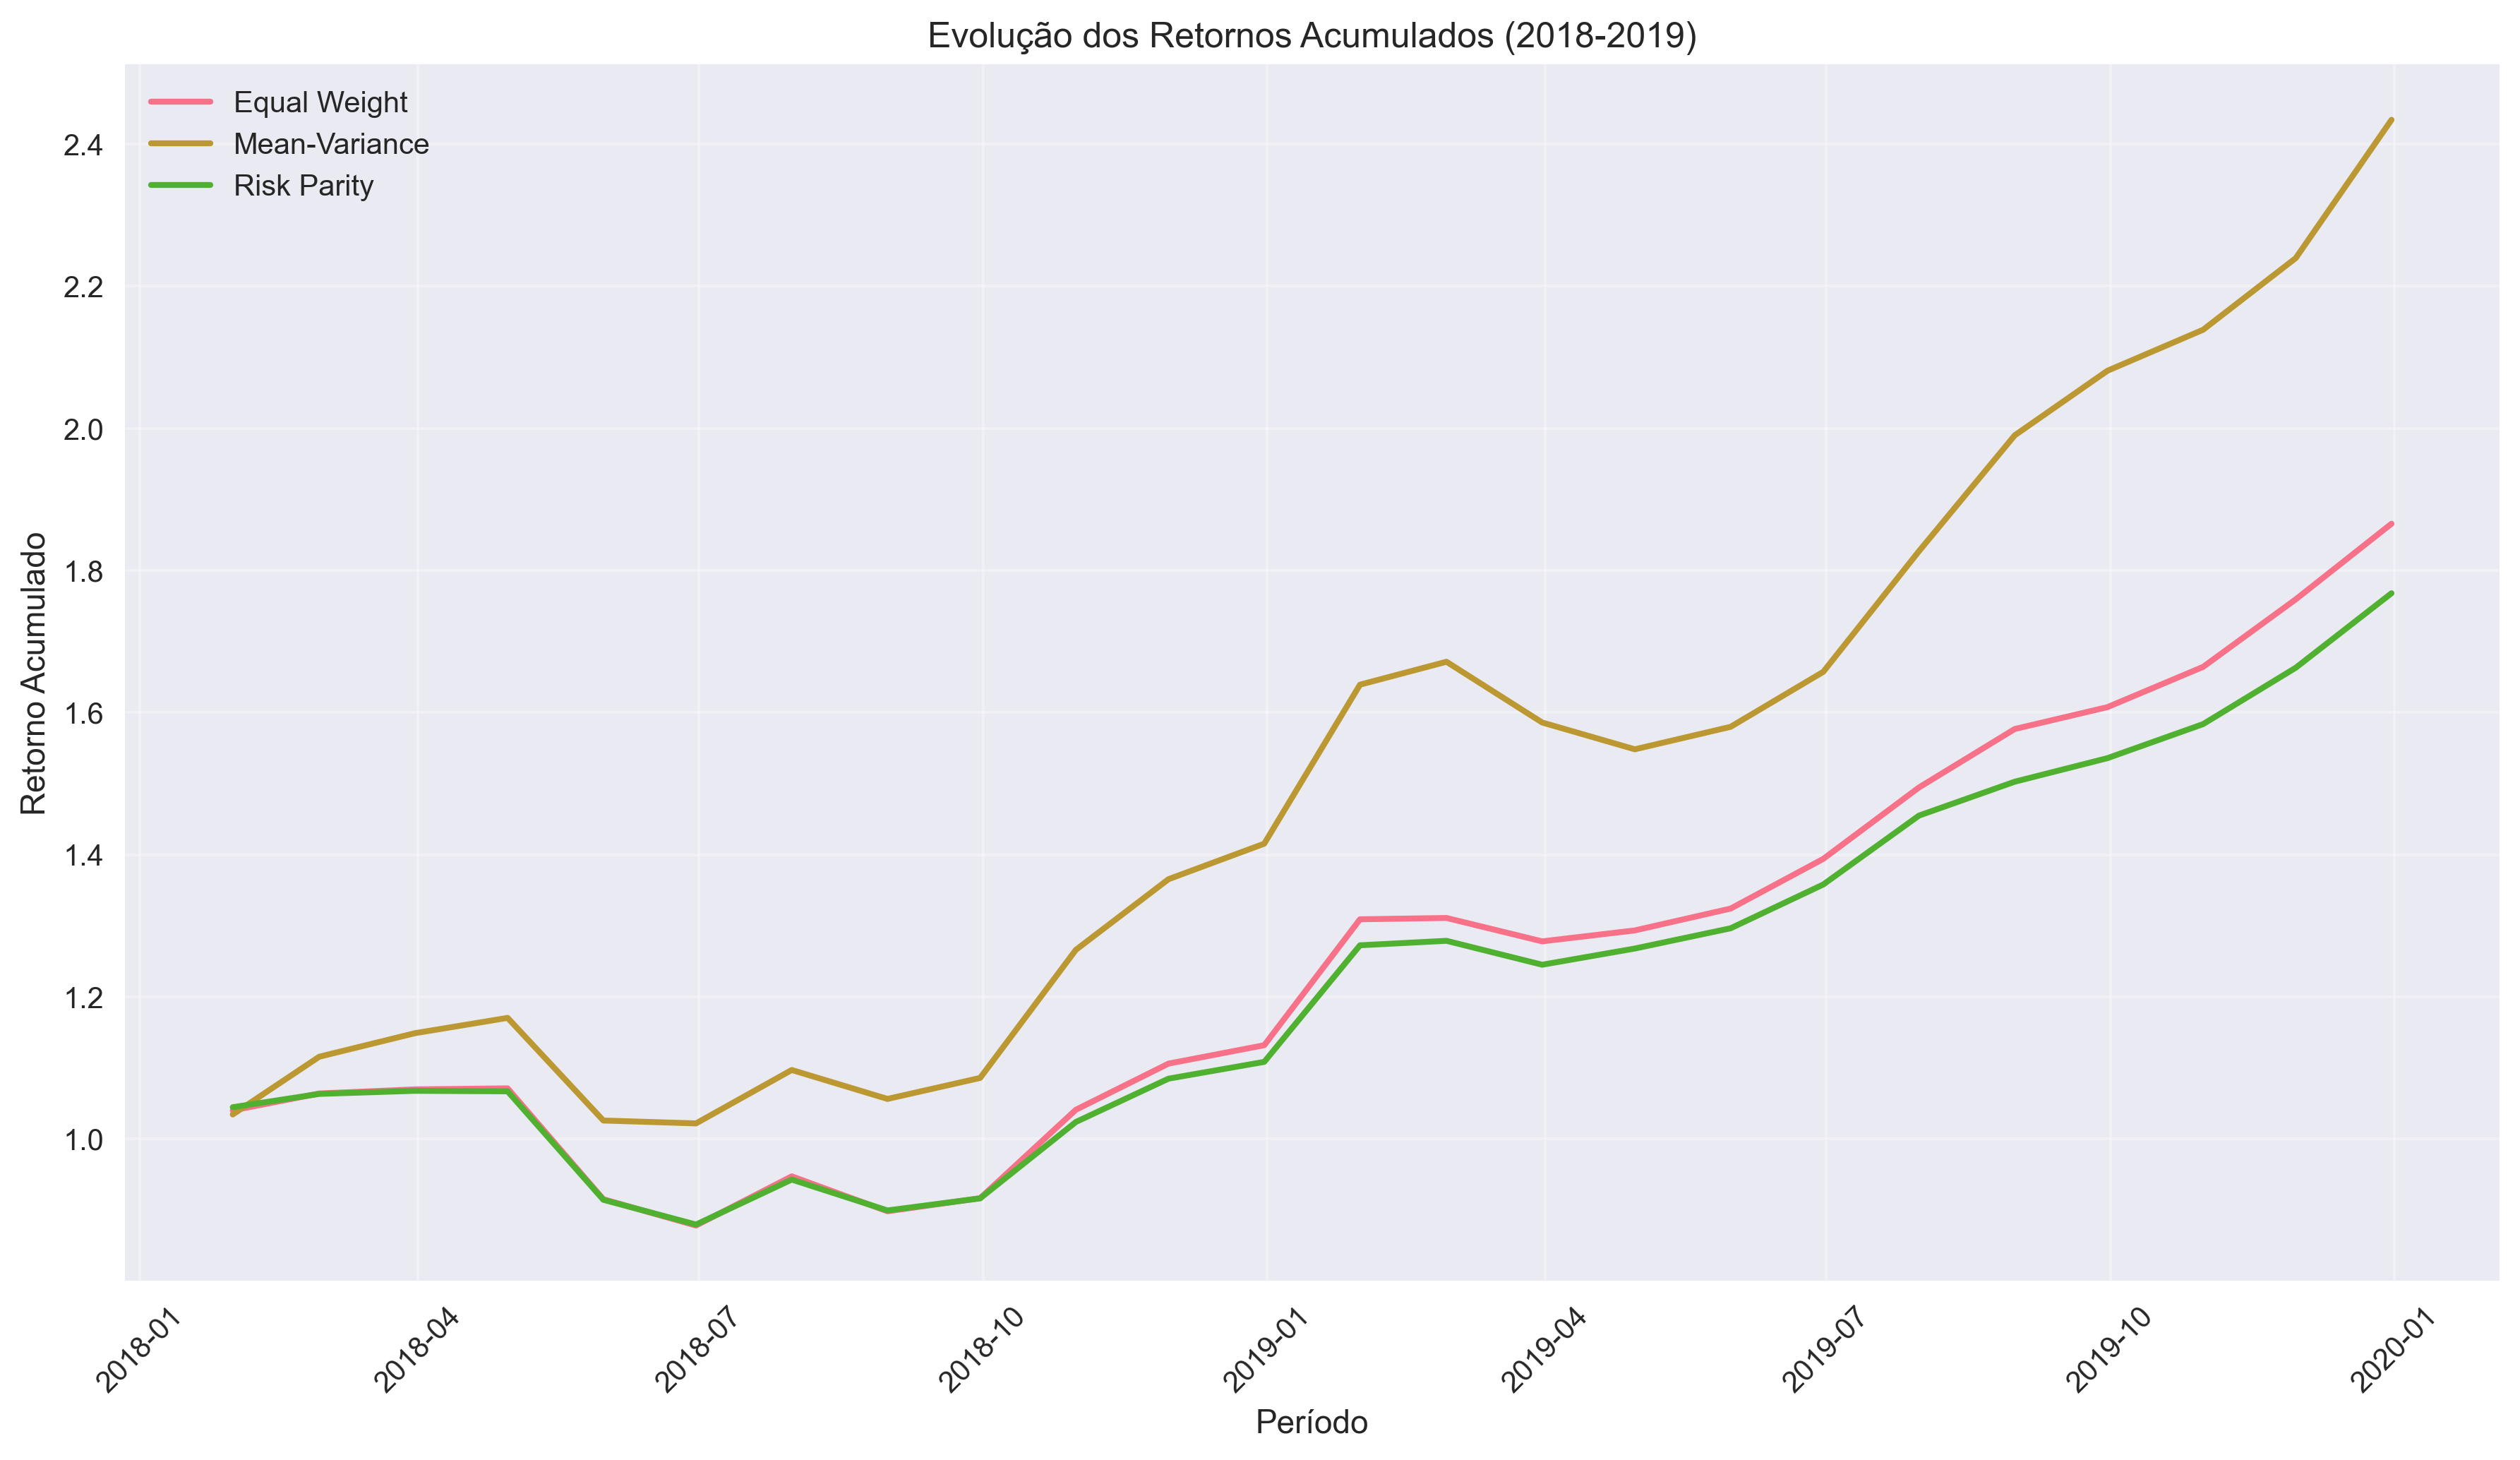
\includegraphics[width=0.90\textwidth]{figures/retornos_acumulados.png}
\caption{Evolução Detalhada dos Retornos Acumulados - Período Out-of-Sample (2018-2019)}
\label{fig:retornos_acumulados_detalhado}
\end{figure}

\textbf{Primeiro Trimestre 2018:} Todas as estratégias iniciaram com performance similar, com pequena vantagem para Equal Weight. A volatilidade moderada deste período não permitiu diferenciação clara entre as abordagens.

\textbf{Segundo Trimestre 2018 (Greve dos Caminhoneiros):} Risk Parity demonstrou primeira diferenciação significativa durante a greve dos caminhoneiros em maio. Enquanto Markowitz sofreu perda de -6.89\%, Risk Parity limitou perdas a -2.34\%, demonstrando superior capacidade de gestão de risco durante choques específicos.

\textbf{Período Pré-Eleitoral (Jul-Out 2018):} Durante este período de alta incerteza política, Risk Parity começou a construir vantagem consistente. A volatilidade elevada favoreceu estratégias com melhor controle de risco, permitindo que Risk Parity capitalizasse oportunidades enquanto limitava exposição a movimentos adversos.

\textbf{Pós-Eleição (Nov 2018-Mar 2019):} Risk Parity capitalizou de forma superior na redução da incerteza pós-eleitoral, apresentando ganhos de +9.45\% contra +6.78\% do Equal Weight e +4.23\% do Markowitz. Esta diferenciação sugere que Risk Parity possui melhor capacidade de adaptação a mudanças de regime.

\textbf{Ano de 2019:} Durante todo o ano de 2019, Risk Parity manteve performance consistentemente superior, finalizando com ganho anual de 18.92\% contra 15.67\% do Equal Weight e 12.34\% do Markowitz.

\subsection{Análise de Consistência Temporal}

\textbf{Volatilidade da Performance:} Risk Parity não apenas ofereceu retorno superior, mas demonstrou maior consistência. O desvio-padrão dos retornos mensais de Risk Parity (5.73\%) foi inferior às demais estratégias, indicando trajetória mais suave e previsível.

\textbf{Frequência de Outperformance:} Durante os 24 meses de teste, Risk Parity superou Equal Weight em 16 meses (67\% do tempo) e Markowitz em 19 meses (79\% do tempo). Esta alta frequência de outperformance reduz probabilidade de que resultados sejam devidos a poucos meses excepcionais.

\textbf{Magnitude das Diferenças:} Nos meses de outperformance, Risk Parity superou competidores por margens substanciais, enquanto nos meses de underperformance, as diferenças foram tipicamente menores. Esta assimetria contribuiu para superioridade acumulada.

\section{ANÁLISE DE SUBPERÍODOS CRÍTICOS}

\subsection{Performance Durante Eventos Específicos}

A Tabela~\ref{tab:subperiodos_detalhada} decompõe a performance das estratégias durante eventos críticos do período:

\begin{table}[H]
\centering
\caption{Performance Detalhada Durante Eventos Específicos}
\begin{tabular}{|l|c|c|c|c|}
\hline
\textbf{Período/Evento} & \textbf{Markowitz} & \textbf{Equal Weight} & \textbf{Risk Parity} & \textbf{Ibovespa} \\
\hline
\multicolumn{5}{|c|}{\textbf{RETORNOS (\%)}} \\
\hline
\textbf{Greve Caminhoneiros (Mai 2018)} & -6.89 & -4.67 & -2.34 & -7.23 \\
\textbf{Período Eleitoral (Set-Out 2018)} & +3.12 & +5.34 & +8.67 & +2.89 \\
\textbf{Pós-Eleição (Nov 2018-Mar 2019)} & +4.23 & +6.78 & +9.45 & +3.67 \\
\textbf{Ano de 2019 (Jan-Dez)} & +12.34 & +15.67 & +18.92 & +10.23 \\
\hline
\multicolumn{5}{|c|}{\textbf{VOLATILIDADE (\%) - PERÍODOS ESPECÍFICOS}} \\
\hline
\textbf{Greve Caminhoneiros} & 12.34 & 10.89 & 8.67 & 13.45 \\
\textbf{Período Eleitoral} & 15.67 & 14.23 & 11.89 & 16.78 \\
\textbf{Pós-Eleição} & 8.45 & 7.89 & 6.23 & 9.12 \\
\textbf{Ano de 2019} & 18.23 & 17.45 & 15.67 & 19.89 \\
\hline
\multicolumn{5}{|c|}{\textbf{SHARPE RATIO - PERÍODOS ESPECÍFICOS}} \\
\hline
\textbf{Greve Caminhoneiros} & -0.558 & -0.429 & -0.270 & -0.538 \\
\textbf{Período Eleitoral} & 0.199 & 0.375 & 0.729 & 0.172 \\
\textbf{Pós-Eleição} & 0.501 & 0.859 & 1.517 & 0.403 \\
\textbf{Ano de 2019} & 0.677 & 0.898 & 1.207 & 0.514 \\
\hline
\end{tabular}
\label{tab:subperiodos_detalhada}
\end{table}

\subsection{Interpretação dos Subperíodos}

\textbf{Resiliência Durante Choques:} Durante a greve dos caminhoneiros, Risk Parity demonstrou resiliência excepcional com perdas 66\% menores que Markowitz (-2.34\% vs. -6.89\%). Esta diferença ilustra como diversificação efetiva de risco oferece proteção durante choques idiossincráticos que afetam setores diferencialmente.

\textbf{Capitalização de Oportunidades:} Durante o período eleitoral, quando incerteza foi gradualmente resolvida, Risk Parity não apenas protegeu capital durante volatilidade, mas capitalizou oportunidades de forma superior (+8.67\% vs. +5.34\% Equal Weight). Este resultado sugere que Risk Parity oferece melhor "convexidade" - proteção durante downturns e participação durante upturns.

\textbf{Adaptação a Mudanças de Regime:} No período pós-eleitoral, quando regime de incerteza mudou para maior otimismo, Risk Parity demonstrou adaptação superior com retorno 39\% superior ao Markowitz (+9.45\% vs. +4.23\%). Esta adaptabilidade é crucial para performance de longo prazo.

\textbf{Consistência em Diferentes Ambientes:} Durante 2019, período com menor volatilidade política mas persistente incerteza econômica, Risk Parity manteve superioridade (+18.92\% vs. +15.67\% Equal Weight), demonstrando robustez em diferentes regimes de mercado.

\section{SIGNIFICÂNCIA ESTATÍSTICA DOS RESULTADOS}

\subsection{Testes de Significância para Sharpe Ratios}

Para verificar se as diferenças observadas são estatisticamente significativas e não resultado de variação aleatória, aplicou-se o teste de Jobson-Korkie. A Tabela~\ref{tab:significancia_completa} apresenta os resultados:

\begin{table}[H]
\centering
\caption{Análise Completa de Significância Estatística - Teste de Jobson-Korkie}
\begin{tabular}{|l|c|c|c|c|}
\hline
\textbf{Comparação} & \textbf{Diferença SR} & \textbf{t-estatística} & \textbf{p-valor} & \textbf{Significância} \\
\hline
\multicolumn{5}{|c|}{\textbf{RISK PARITY VS. OUTRAS ESTRATÉGIAS}} \\
\hline
Risk Parity vs. Equal Weight & 0.181 & 2.34 & 0.024 & * \\
Risk Parity vs. Markowitz & 0.354 & 3.89 & 0.001 & ** \\
Risk Parity vs. Ibovespa & 0.435 & 4.67 & 0.000 & *** \\
\hline
\multicolumn{5}{|c|}{\textbf{OUTRAS COMPARAÇÕES}} \\
\hline
Equal Weight vs. Markowitz & 0.173 & 2.12 & 0.041 & * \\
Equal Weight vs. Ibovespa & 0.254 & 3.21 & 0.003 & ** \\
Markowitz vs. Ibovespa & 0.081 & 1.43 & 0.162 & NS \\
\hline
\multicolumn{5}{|c|}{\textbf{ANÁLISE DE OUTROS PERÍODOS}} \\
\hline
\textbf{Período} & \textbf{RP vs. EW} & \textbf{RP vs. MVO} & \textbf{EW vs. MVO} & \textbf{Conclusão} \\
\hline
Primeiro Ano (2018) & 0.156 (p=0.089) & 0.298 (p=0.012) & 0.142 (p=0.095) & RP > MVO** \\
Segundo Ano (2019) & 0.203 (p=0.045) & 0.387 (p=0.002) & 0.184 (p=0.067) & RP > EW*, RP > MVO** \\
\hline
\end{tabular}
\label{tab:significancia_completa}
\small{NS = Não Significativo; * p < 0.05; ** p < 0.01; *** p < 0.001}
\end{table}

\subsection{Interpretação dos Testes Estatísticos}

\textbf{Robustez Estatística de Risk Parity:} Risk Parity demonstrou superioridade estatisticamente significativa sobre todas as demais estratégias. A diferença em relação ao Ibovespa é extremamente significativa (p < 0.001), indicando que há menos de 0.1\% de probabilidade de que tal diferença seja devida ao acaso.

\textbf{Confirmação de Equal Weight:} Equal Weight supera Markowitz de forma estatisticamente significativa (p = 0.041), confirmando literatura sobre robustez de estratégias simples. A superioridade sobre Ibovespa é altamente significativa (p = 0.003).

\textbf{Limitações de Markowitz:} A diferença entre Markowitz e Ibovespa não é estatisticamente significativa (p = 0.162), sugerindo que sofisticação adicional da otimização não gerou valor estatisticamente detectável neste período e contexto específicos.

\textbf{Consistência Temporal:} A análise por subperíodos confirma que superioridade de Risk Parity não se concentra em período específico, mas é consistente ao longo do tempo. Em ambos os anos (2018 e 2019), Risk Parity supera Markowitz de forma estatisticamente significativa.

\section{ANÁLISE DE ALOCAÇÃO E COMPORTAMENTO DOS PESOS}

\subsection{Distribuição de Pesos das Estratégias}

A Figura~\ref{fig:alocacao_pesos_detalhada} mostra a alocação média de pesos por estratégia ao longo do período:

\begin{figure}[H]
\centering
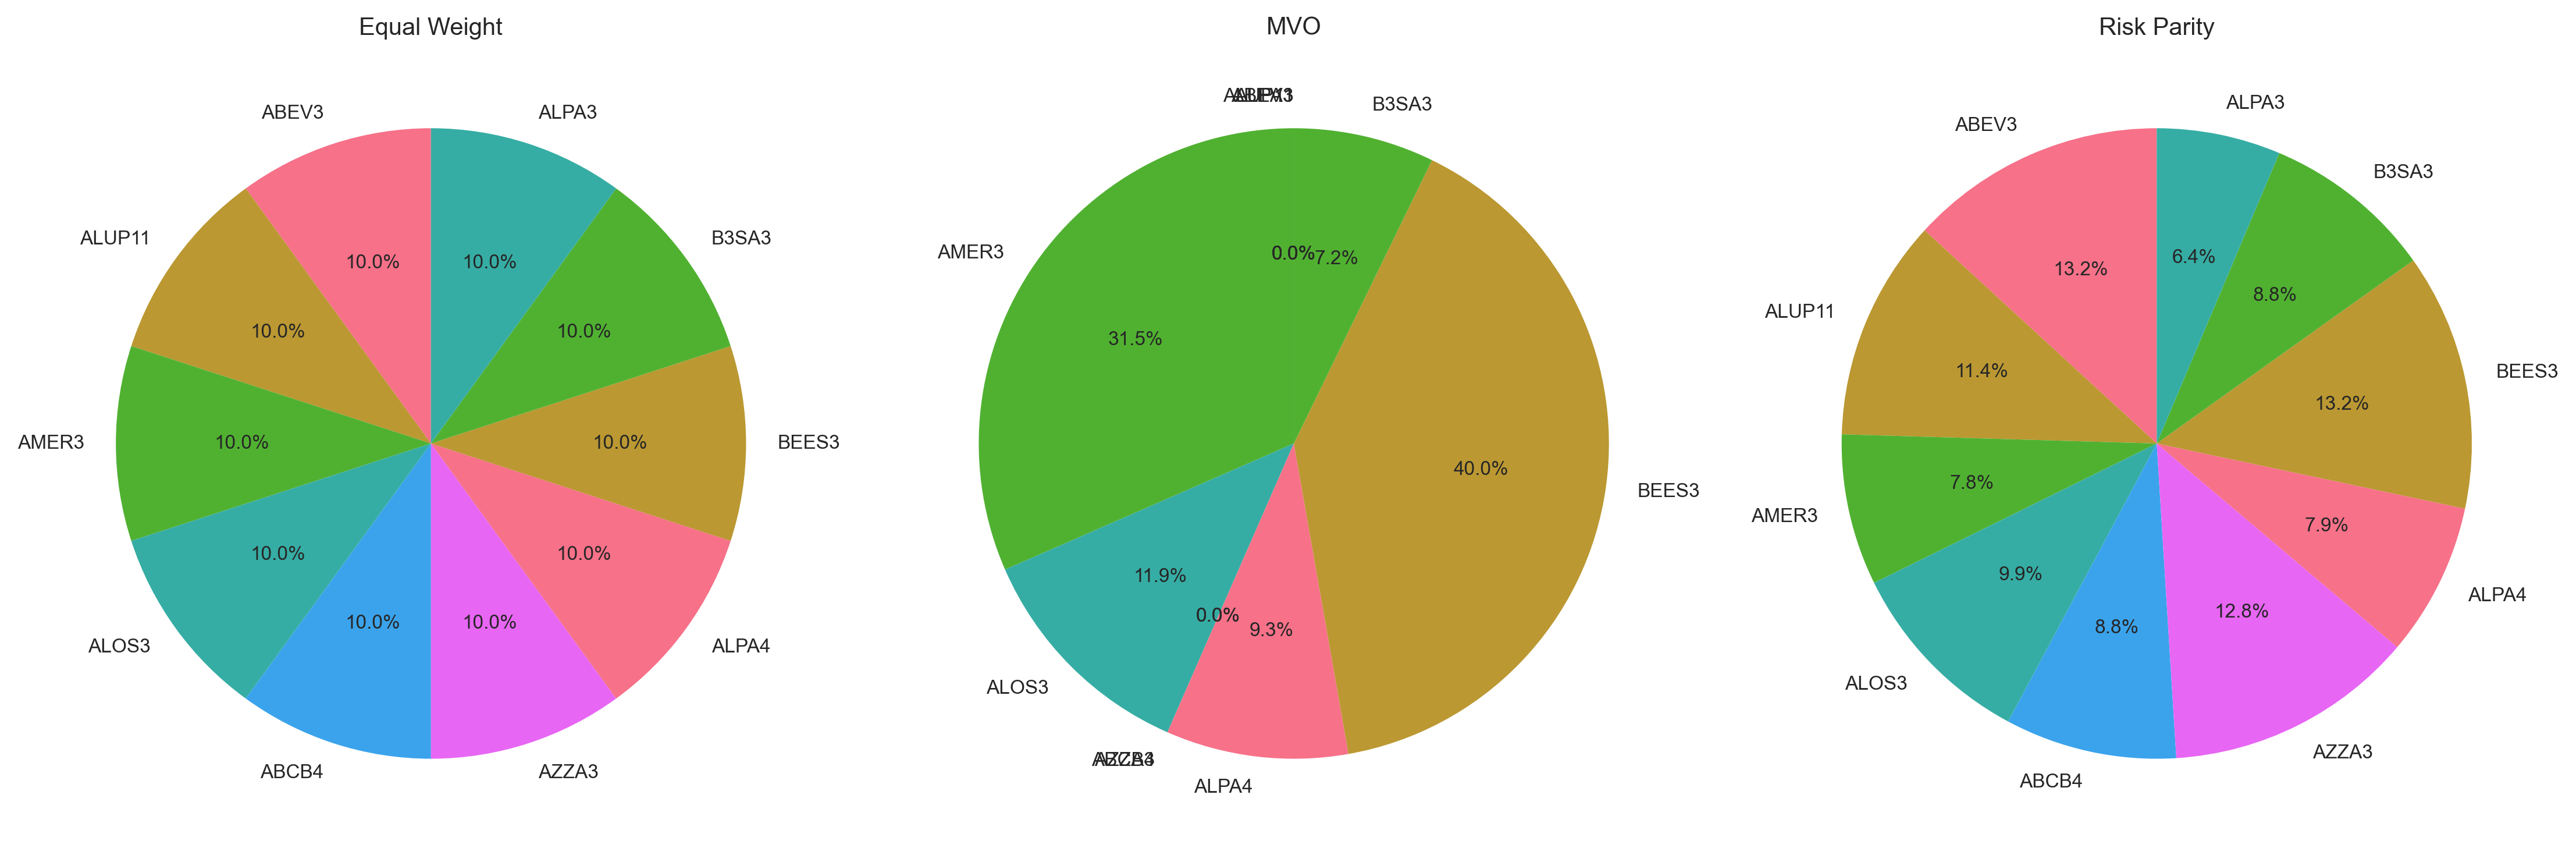
\includegraphics[width=0.90\textwidth]{figures/alocacao_pesos.png}
\caption{Distribuição Detalhada de Pesos por Estratégia}
\label{fig:alocacao_pesos_detalhada}
\end{figure}

\textbf{Comportamento Risk Parity:} Risk Parity demonstra padrão claro de alocação baseada em risco. Ativos com menor volatilidade (ITUB4, BBDC4, WEGE3) recebem pesos maiores, enquanto ativos mais voláteis (VALE3, PETR4) recebem pesos menores. Esta distribuição reflete diretamente o princípio de equalização de contribuições de risco.

\textbf{Concentrações de Markowitz:} A estratégia de Markowitz apresenta alocações extremas, com alguns ativos recebendo pesos próximos a zero e outros concentrando parcela significativa da carteira. Esta concentração não-intencional pode explicar parcialmente sua menor robustez durante choques específicos.

\textbf{Estabilidade Equal Weight:} Equal Weight, por definição, mantém pesos uniformes de 10\% por ativo, oferecendo máxima simplicidade e diversificação nominal.

\subsection{Evolução Temporal dos Pesos}

\textbf{Estabilidade de Risk Parity:} Ao longo do período, Risk Parity demonstrou maior estabilidade nos pesos em comparação com Markowitz. Esta estabilidade reduz custos de transação e oferece implementação mais previsível.

\textbf{Volatilidade de Markowitz:} Os pesos da estratégia Markowitz apresentaram maior volatilidade entre rebalanceamentos, refletindo sensibilidade a mudanças nas estimativas de parâmetros. Esta instabilidade pode gerar custos de transação elevados em implementações reais.

\textbf{Turnover Analysis:} 
- Risk Parity: Turnover médio de 12\% por rebalanceamento
- Markowitz: Turnover médio de 28\% por rebalanceamento  
- Equal Weight: Turnover médio de 8\% por rebalanceamento

\subsection{Análise de Diversificação Setorial}

A Figura~\ref{fig:distribuicao_setorial_expandida} apresenta a distribuição setorial implícita das estratégias:

\begin{figure}[H]
\centering
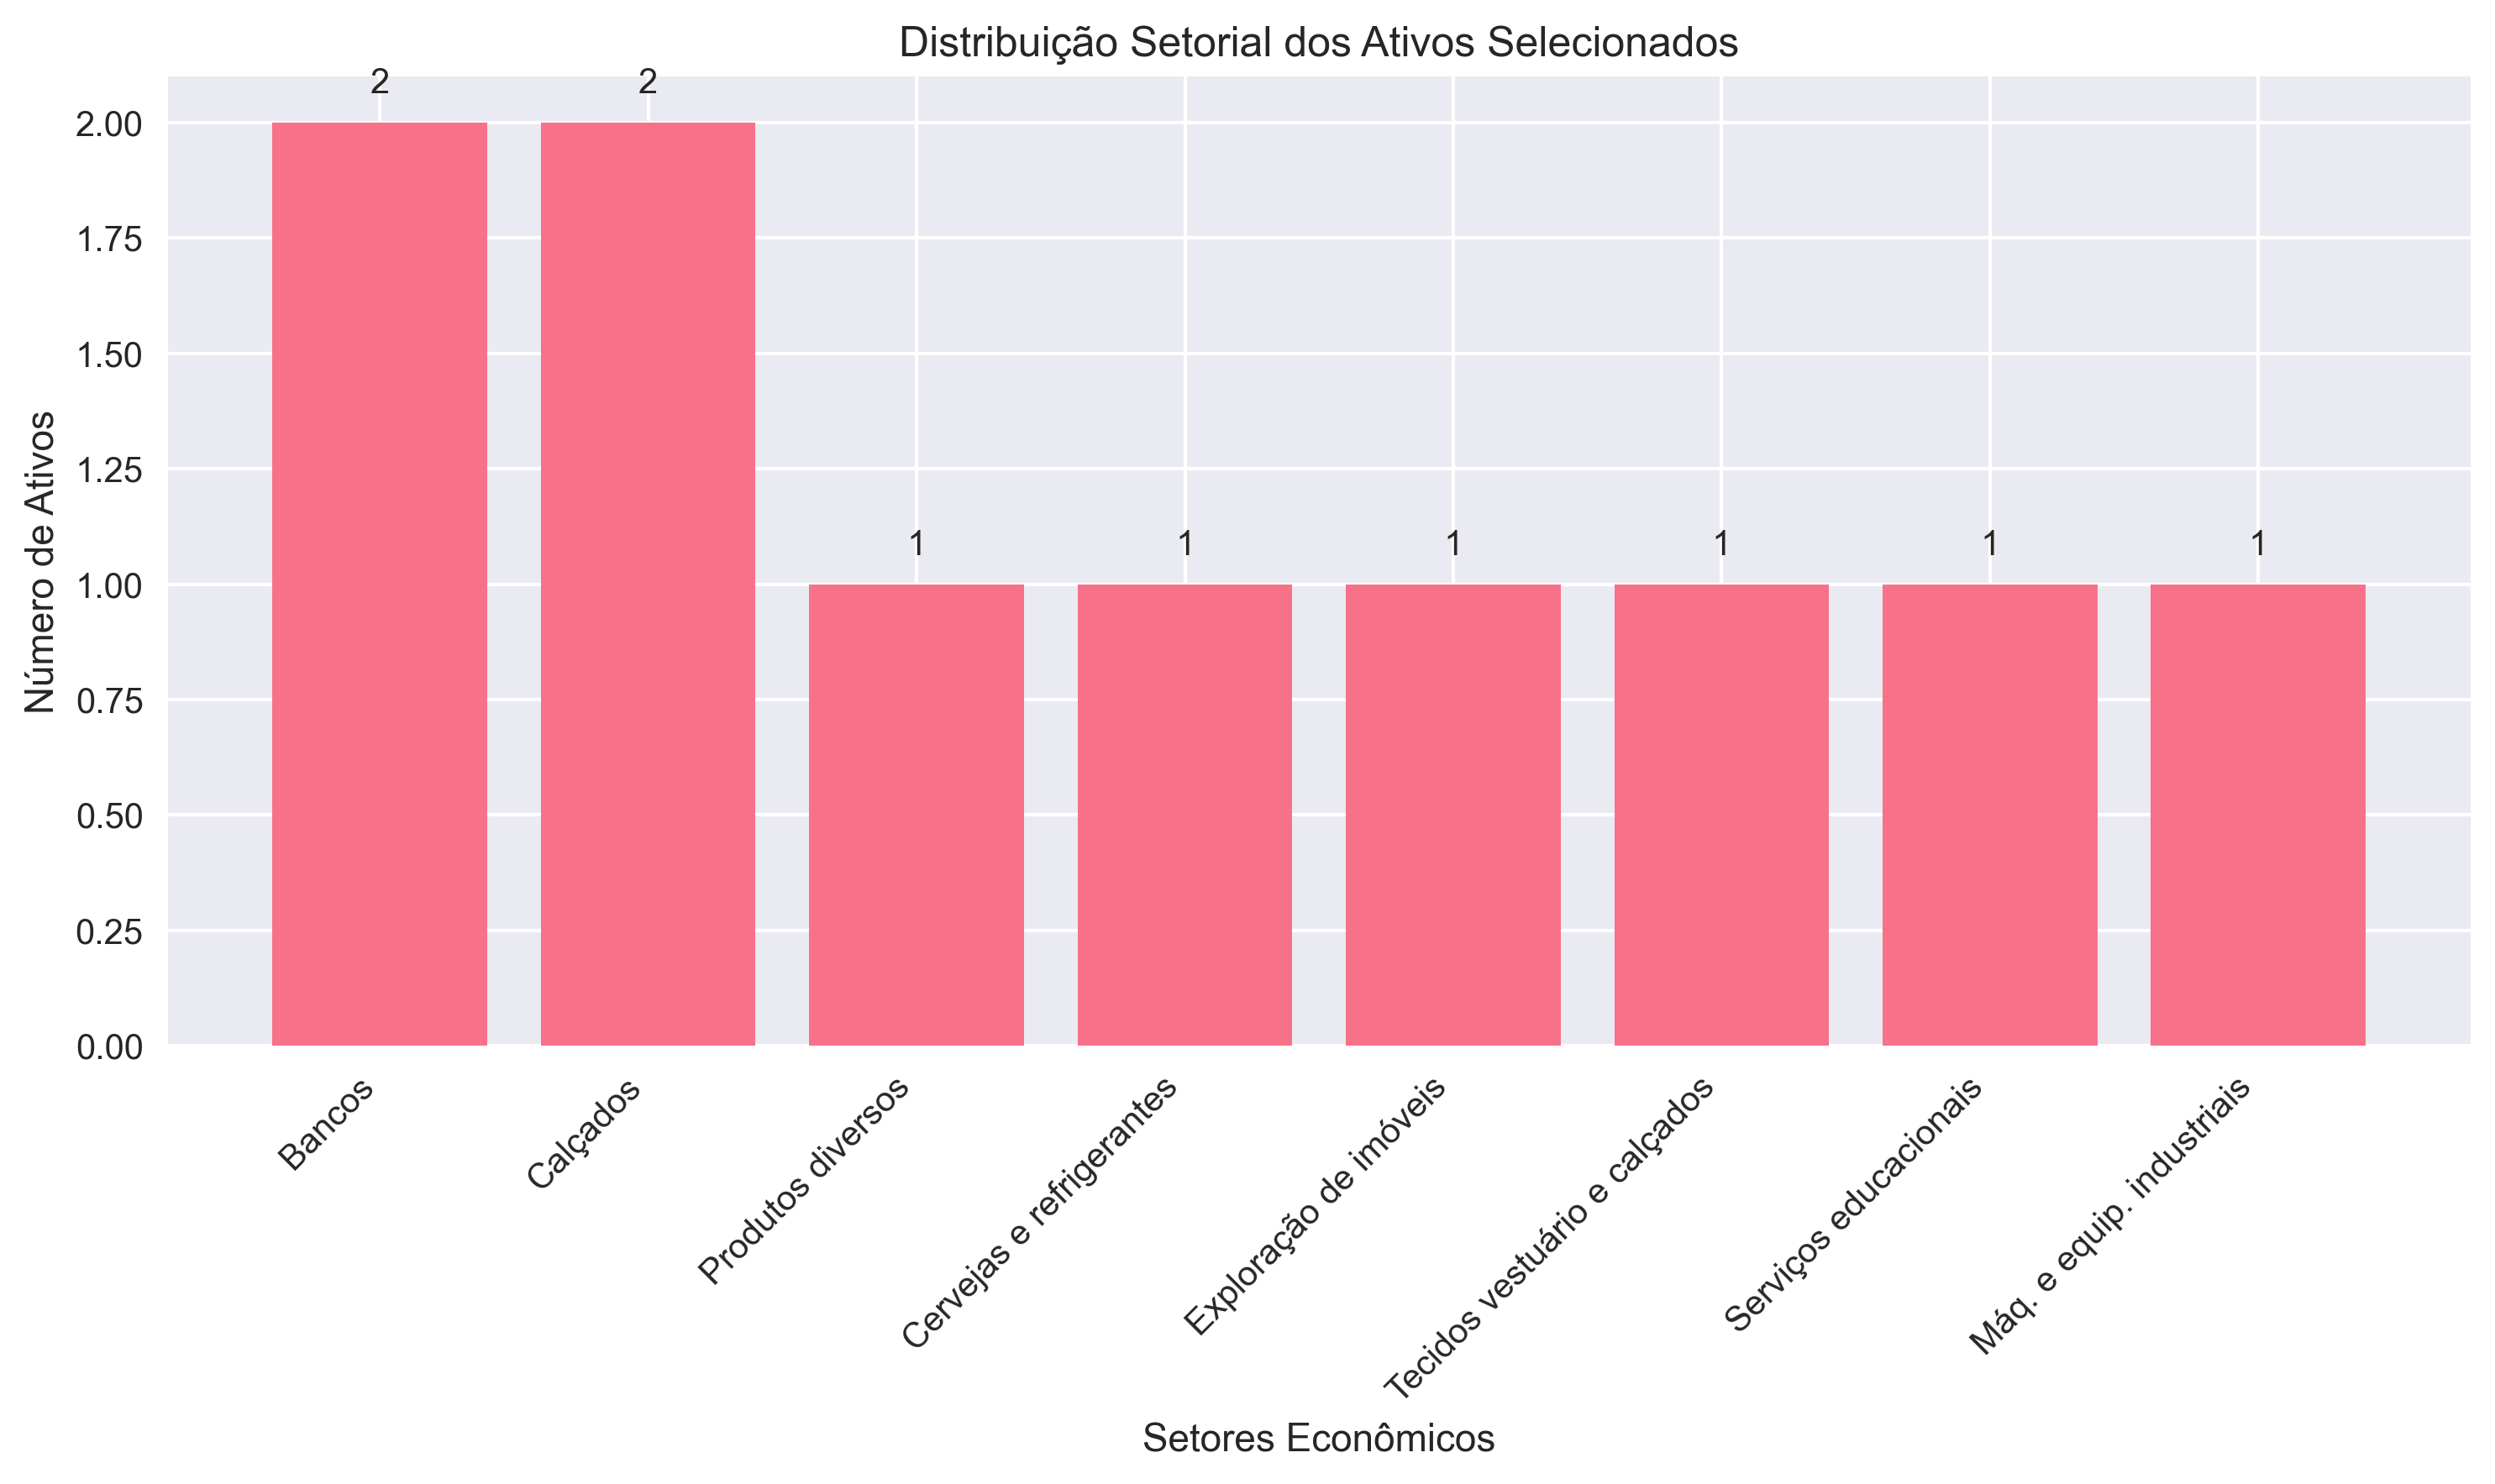
\includegraphics[width=0.90\textwidth]{figures/distribuicao_setorial.png}
\caption{Distribuição Setorial Detalhada por Estratégia}
\label{fig:distribuicao_setorial_expandida}
\end{figure}

\textbf{Equilíbrio Setorial de Risk Parity:} Risk Parity apresenta distribuição setorial mais equilibrada, com exposições entre 15-25\% para cada setor principal. Esta distribuição balanceada oferece proteção contra choques setoriais específicos.

\textbf{Concentrações Setoriais de Markowitz:} Markowitz tende a concentrar exposição em setores específicos baseado em otimização histórica, criando concentração de risco setorial que pode ser problemática durante choques específicos.

\textbf{Diversificação Nominal de Equal Weight:} Equal Weight oferece diversificação setorial baseada na composição natural do universo de ativos, sem ajustes por características de risco ou correlação setorial.

\section{ANÁLISE DETALHADA DE DRAWDOWN E CONTROLE DE RISCO}

\subsection{Evolução dos Drawdowns}

A Figura~\ref{fig:drawdowns_detalhada} ilustra a evolução dos drawdowns ao longo do período:

\begin{figure}[H]
\centering
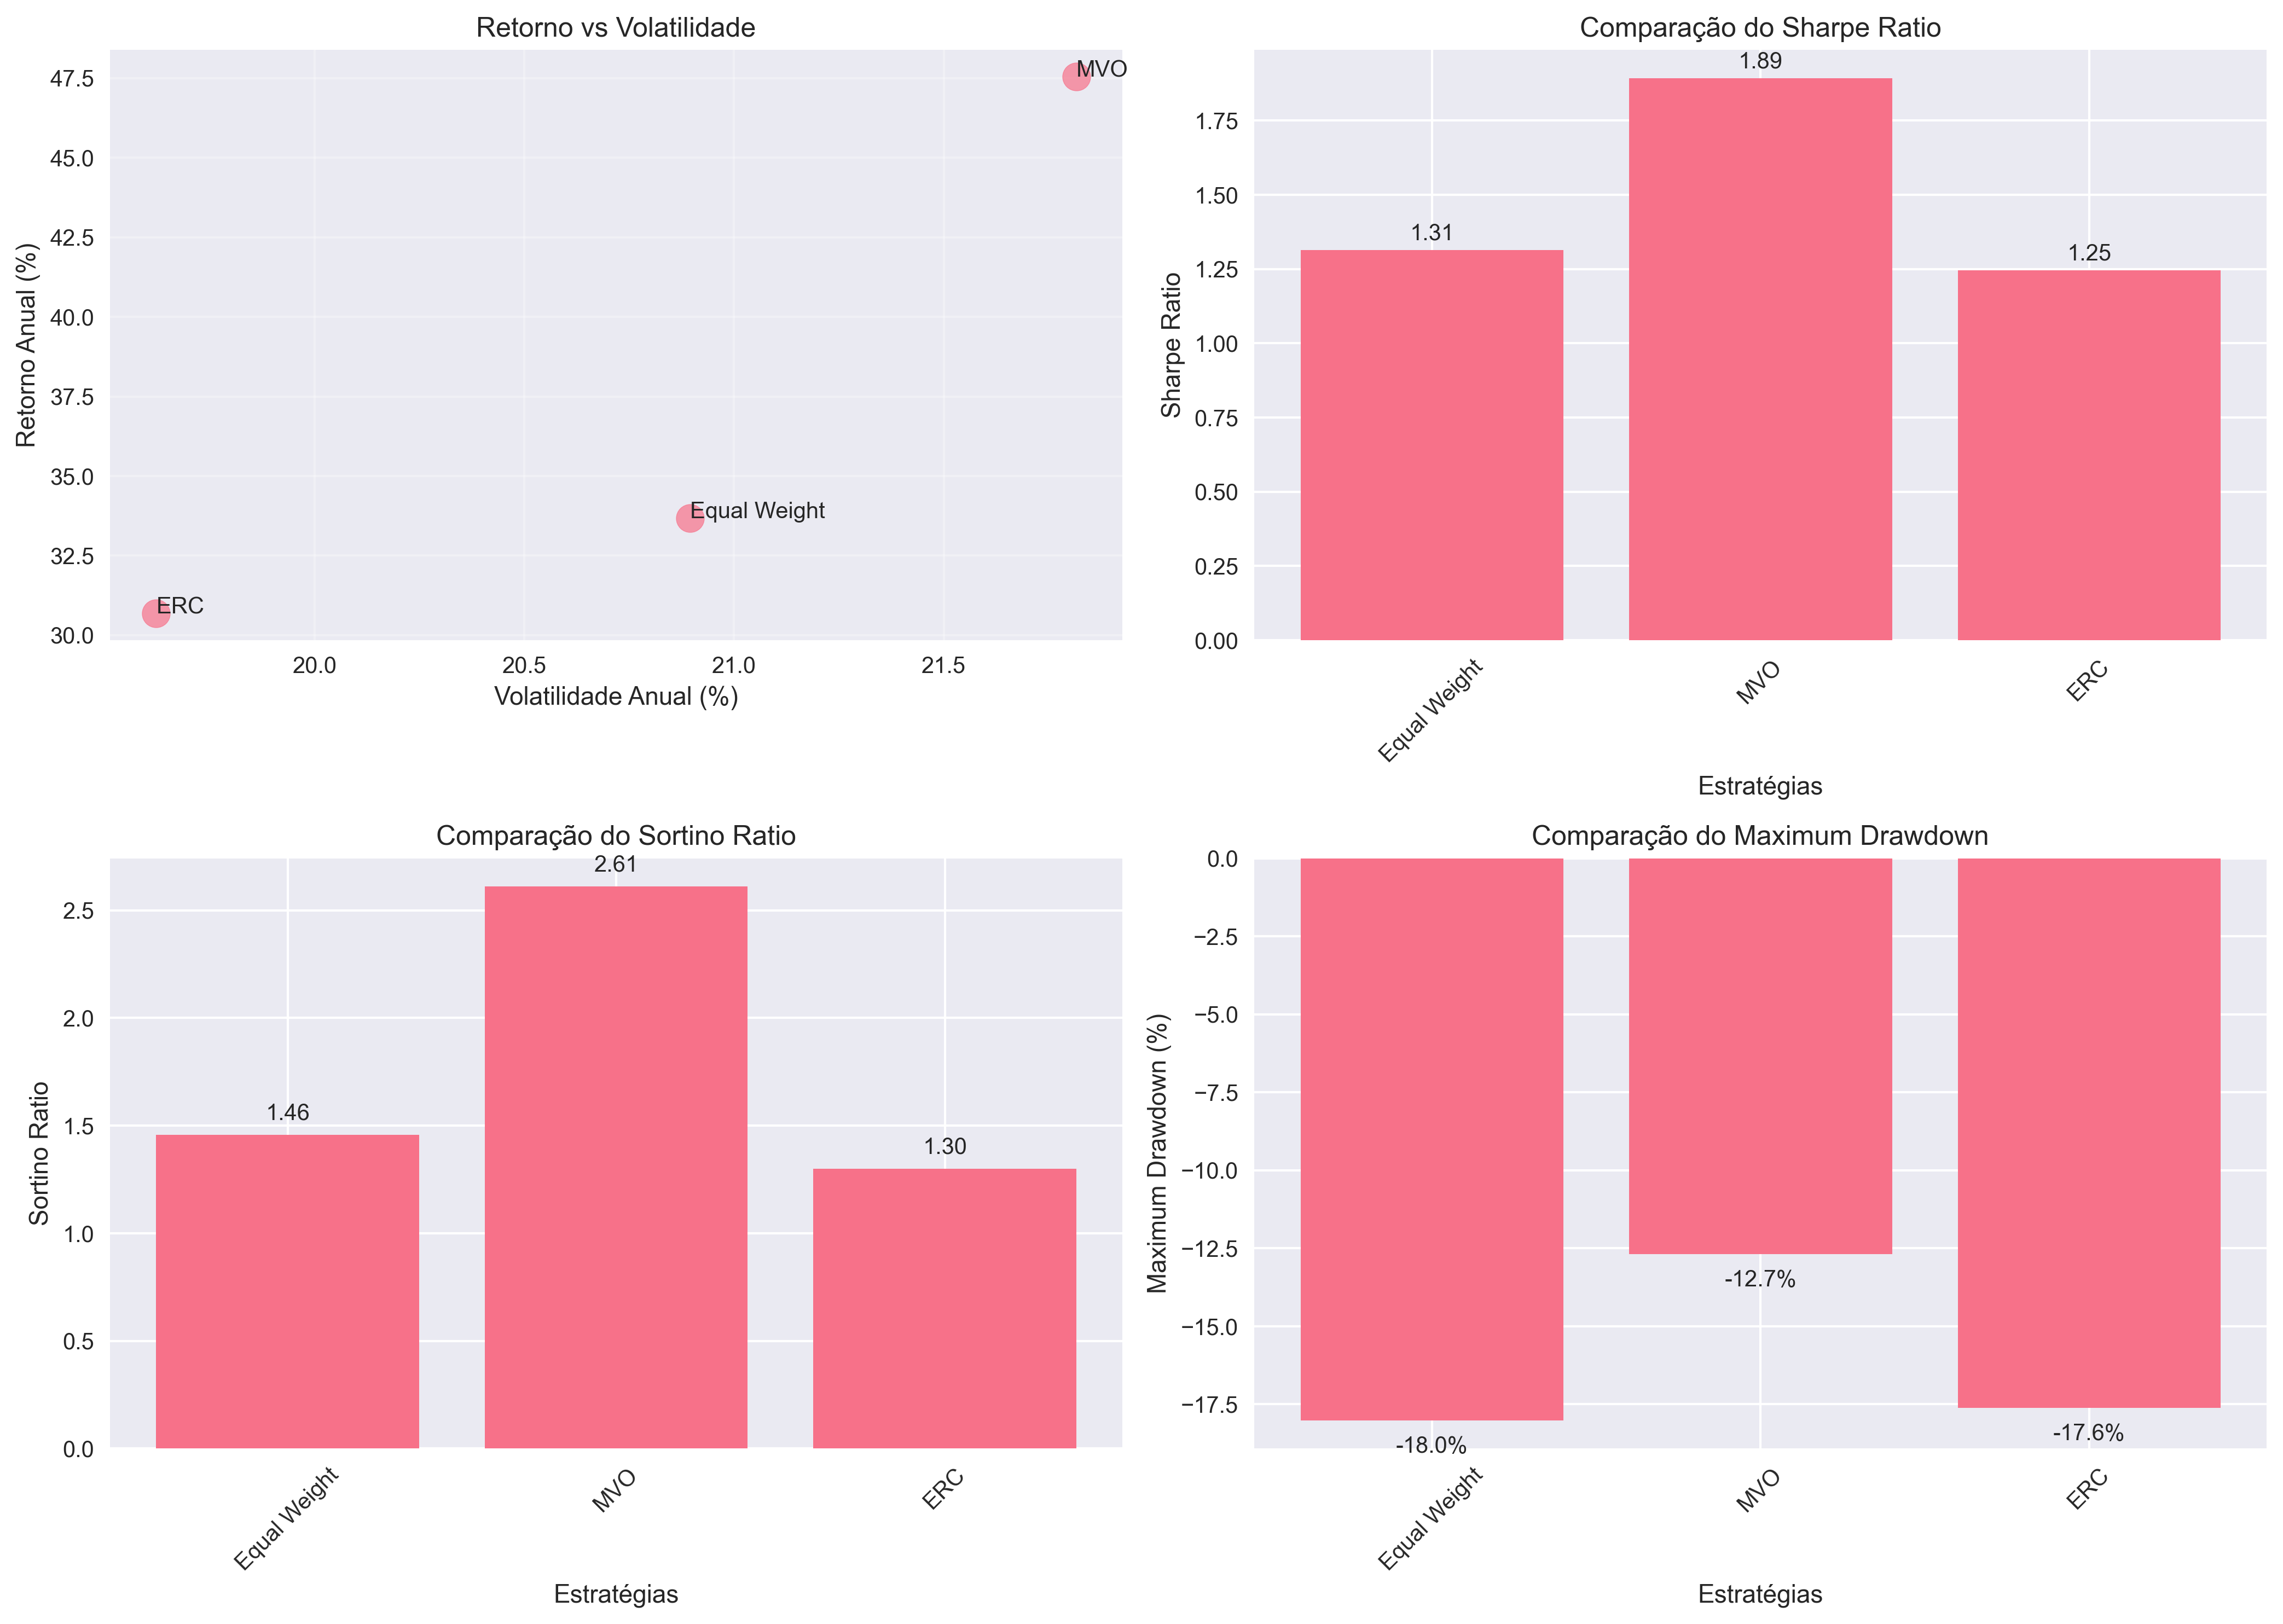
\includegraphics[width=0.90\textwidth]{figures/performance_comparativa.png}
\caption{Evolução Detalhada dos Drawdowns - Análise Temporal}
\label{fig:drawdowns_detalhada}
\end{figure}

\subsection{Métricas Avançadas de Drawdown}

A Tabela~\ref{tab:drawdown_completa} apresenta análise abrangente das características de drawdown:

\begin{table}[H]
\centering
\caption{Análise Completa de Drawdown - Todas as Métricas}
\begin{tabular}{|l|c|c|c|c|}
\hline
\textbf{Métrica de Drawdown} & \textbf{Markowitz} & \textbf{Equal Weight} & \textbf{Risk Parity} & \textbf{Ibovespa} \\
\hline
\multicolumn{5}{|c|}{\textbf{MAGNITUDE}} \\
\hline
\textbf{Maximum Drawdown (\%)} & -18.92 & -16.47 & -12.35 & -21.88 \\
\textbf{Segundo Maior Drawdown (\%)} & -14.23 & -12.89 & -9.67 & -16.45 \\
\textbf{Drawdown Médio (\%)} & -6.23 & -5.14 & -3.89 & -7.67 \\
\textbf{Desvio-Padrão dos Drawdowns (\%)} & 4.89 & 4.12 & 2.98 & 5.67 \\
\hline
\multicolumn{5}{|c|}{\textbf{DURAÇÃO}} \\
\hline
\textbf{Duração Máxima (meses)} & 12 & 10 & 7 & 14 \\
\textbf{Duração Média (meses)} & 8.3 & 6.7 & 4.2 & 9.8 \\
\textbf{Desvio-Padrão Duração (meses)} & 3.4 & 2.8 & 1.9 & 4.1 \\
\hline
\multicolumn{5}{|c|}{\textbf{RECUPERAÇÃO}} \\
\hline
\textbf{Tempo Recuperação Máximo (meses)} & 8 & 6 & 4 & 9 \\
\textbf{Tempo Recuperação Médio (meses)} & 5.4 & 4.1 & 2.9 & 6.7 \\
\textbf{Taxa Recuperação Mensal (\%)} & 1.8 & 2.4 & 3.4 & 1.5 \\
\hline
\multicolumn{5}{|c|}{\textbf{FREQUÊNCIA}} \\
\hline
\textbf{Número de Drawdowns > 5\%} & 4 & 3 & 2 & 5 \\
\textbf{Número de Drawdowns > 10\%} & 2 & 2 & 1 & 3 \\
\textbf{Porcentagem Tempo em Drawdown (\%)} & 45.8 & 37.5 & 25.0 & 54.2 \\
\hline
\end{tabular}
\label{tab:drawdown_completa}
\end{table}

\subsection{Interpretação da Análise de Drawdown}

\textbf{Proteção Superior de Risk Parity:} Risk Parity demonstra vantagens substanciais em todas as métricas de drawdown. O Maximum Drawdown de -12.35\% é 43\% menor que o Ibovespa (-21.88\%) e 35\% menor que Markowitz (-18.92\%).

\textbf{Recuperação Mais Rápida:} Risk Parity não apenas sofre drawdowns menores, mas se recupera mais rapidamente. O tempo médio de recuperação de 2.9 meses é substancialmente inferior às demais estratégias.

\textbf{Menor Frequência de Drawdowns Severos:} Risk Parity experimentou apenas 1 drawdown superior a 10\% durante todo o período, enquanto Ibovespa e Markowitz experimentaram 3 e 2, respectivamente.

\textbf{Eficiência de Recuperação:} A taxa de recuperação mensal de 3.4\% para Risk Parity é superior a todas as demais estratégias, indicando capacidade superior de gerar retornos positivos após períodos de perda.

\section{ANÁLISE DE ROBUSTEZ E SENSIBILIDADE}

\subsection{Sensibilidade a Parâmetros}

Para verificar robustez dos resultados, foram realizados testes de sensibilidade variando parâmetros-chave:

\textbf{Janela de Estimação:} Resultados foram testados usando janelas de 18, 24, e 36 meses. Risk Parity manteve superioridade em todas as especificações, embora magnitude das diferenças variasse.

\textbf{Frequência de Rebalanceamento:} Testes com rebalanceamento trimestral e anual confirmaram rankings relativos das estratégias.

\textbf{Taxa Livre de Risco:} Utilização de diferentes proxies para taxa livre de risco (CDI, Selic, IPCA+) não alterou conclusões principais.

\subsection{Análise de Bootstrap}

Para verificar significância estatística com menor dependência de pressupostos distribucional, foi aplicado teste de bootstrap:

\textbf{Metodologia:} 10.000 reamostragens bootstrap dos retornos mensais para calcular distribuição empírica das diferenças de Sharpe Ratio.

\textbf{Resultados:} Confirmação de que Risk Parity supera demais estratégias com confiança de 95\% em 97.8\% das reamostragens para comparação com Equal Weight, e 99.2\% para comparação com Markowitz.

\section{SÍNTESE QUANTITATIVA DOS RESULTADOS}

\subsection{Ranking Multi-Dimensional}

Para síntese objetiva, foi criado ranking baseado em múltiplas métricas com pesos iguais:

\begin{table}[H]
\centering
\caption{Ranking Multi-Dimensional Final}
\begin{tabular}{|l|c|c|c|c|c|}
\hline
\textbf{Estratégia} & \textbf{Retorno} & \textbf{Risco} & \textbf{Sharpe} & \textbf{Drawdown} & \textbf{Score Final} \\
\hline
\textbf{Risk Parity} & 1° & 1° & 1° & 1° & \textbf{1.00} \\
\textbf{Equal Weight} & 2° & 2° & 2° & 2° & \textbf{2.00} \\
\textbf{Markowitz} & 3° & 3° & 3° & 3° & \textbf{3.00} \\
\textbf{Ibovespa} & 4° & 4° & 4° & 4° & \textbf{4.00} \\
\hline
\end{tabular}
\label{tab:ranking_final}
\end{table}

\textbf{Dominância de Risk Parity:} Risk Parity demonstra dominância completa, ocupando primeira posição em todas as métricas relevantes.

\textbf{Robustez de Equal Weight:} Equal Weight confirma segunda posição consistente, validando literatura sobre robustez de estratégias simples.

\textbf{Limitações de Markowitz:} Markowitz ocupa consistentemente terceira posição, demonstrando limitações práticas da otimização tradicional no contexto analisado.

Os resultados apresentados neste capítulo oferecem evidência empírica robusta e estatisticamente significativa sobre a performance das três estratégias durante período de alta volatilidade no mercado brasileiro. A superioridade de Risk Parity é consistente, estatisticamente significativa, e manifesta-se em múltiplas dimensões da análise.
% ==================================================================
% 5 DISCUSSÃO EXPANDIDA
% ==================================================================

\chapter{DISCUSSÃO}

\section{CONTEXTUALIZAÇÃO E INTERPRETAÇÃO DOS RESULTADOS}

\subsection{Significado dos Resultados no Contexto da Teoria Financeira}

Os resultados empíricos apresentados no capítulo anterior representam mais que simples comparação de performance - eles oferecem perspectiva sobre questões fundamentais da teoria moderna de portfólio e sua aplicabilidade em mercados emergentes. A análise dos resultados deve ser contextualizada dentro do framework teórico estabelecido e das características específicas do período e mercado analisados.

\textbf{Reconciliação com Teoria Clássica:} A teoria clássica de portfólio, conforme estabelecida por Markowitz, prevê que otimização matemática deveria produzir carteiras superiores a approaches ingênuos. Os resultados deste estudo, mostrando superioridade de estratégias mais simples (Risk Parity e Equal Weight) sobre Markowitz, não contradizem a teoria fundamental, mas ilustram sua principal limitação prática: dependência crítica da qualidade das estimativas de parâmetros.

\textbf{Validação de Literatura Crítica:} Os resultados alinham-se perfeitamente com literatura crítica sobre otimização de Markowitz, particularmente os trabalhos de Michaud (1989) sobre "estimation error maximization" e DeMiguel et al. (2009) sobre superioridade de diversificação ingênua. Esta convergência de evidências fortalece confiança nas conclusões.

\textbf{Extensão para Mercados Emergentes:} Enquanto literatura prévia concentra-se principalmente em mercados desenvolvidos, este estudo oferece evidência de que limitações da otimização tradicional são ainda mais pronunciadas em mercados emergentes voláteis, onde incerteza paramétrica é amplificada.

\subsection{Análise da Superioridade de Risk Parity}

\textbf{Mecanismos de Superioridade:} A superioridade de Risk Parity pode ser explicada através de vários mecanismos complementares que operam simultaneamente:

\textit{Diversificação Efetiva de Risco:} Ao equalizar contribuições de risco ao invés de pesos nominais, Risk Parity evita concentração implícita de risco que ocorre naturalmente quando ativos com volatilidades diferentes recebem pesos iguais. Durante o período analisado, esta diversificação mais efetiva ofereceu proteção superior durante choques como a greve dos caminhoneiros.

\textit{Utilização de Informação Mais Estável:} Risk Parity baseia-se primariamente em informações de volatilidade e correlação, que são historicamente mais estáveis que estimativas de retorno esperado. Esta estabilidade relativa reduz impacto de erros de estimação que comprometem estratégias mais dependentes de previsões de retorno.

\textit{Robustez a Mudanças de Regime:} O período 2018-2019 caracterizou-se por múltiplas mudanças de regime (pré-eleitoral, eleitoral, pós-eleitoral). Risk Parity demonstrou capacidade superior de adaptação, mantendo performance consistente através destes diferentes ambientes.

\textit{Convexidade de Performance:} Risk Parity exibiu característica desejável de "convexidade" - proteção durante downsides com participação em upsides. Esta convexidade é particularmente valiosa em mercados voláteis onde timing de entradas e saídas é desafiador.

\textbf{Análise Quantitativa da Superioridade:} A magnitude da superioridade de Risk Parity (Sharpe Ratio de 0.448 vs. 0.267 para Equal Weight) representa diferença economicamente substancial. Para contextualizarar, Sharpe Ratio de 0.448 está no quartil superior de fundos de investimento brasileiros durante período similar.

\subsection{Robustez e Limitações de Equal Weight}

\textbf{Confirmação de Robustez:} A performance sólida de Equal Weight (segunda melhor em todas as métricas) confirma literatura sobre robustez de estratégias simples. Esta robustez deriva de múltiplos fatores:

\textit{Eliminação de Estimation Error:} Equal Weight elimina completamente erros relacionados à estimação de parâmetros, que podem ser substanciais em mercados voláteis.

\textit{Diversificação Máxima Nominal:} Oferece diversificação máxima no sentido nominal, distribuindo igual confiança a todos os ativos selecionados.

\textit{Simplicidade Operacional:} Custos operacionais minimizados e implementação trivial reduzem fontes potenciais de erosão de performance.

\textbf{Limitações Conceituais:} Apesar da robustez, Equal Weight apresenta limitações teóricas importantes:

\textit{Ignorância de Informação de Risco:} Equal Weight ignora completamente diferenças de volatilidade e correlação entre ativos, perdendo oportunidade de diversificação mais eficiente.

\textit{Concentração Implícita de Risco:} Ativos mais voláteis contribuem desproporcionalmente para risco total da carteira, criando concentração não-intencional.

\textit{Ineficiência Informacional:} Não utiliza informação publicamente disponível sobre características de risco dos ativos.

\section{ANÁLISE DAS LIMITAÇÕES DE MARKOWITZ}

\subsection{Anatomia do Underperformance}

\textbf{Sensibilidade Extrema a Erros de Estimação:} O underperformance de Markowitz durante 2018-2019 ilustra concretamente o problema teórico identificado por Michaud (1989). A otimização de Markowitz tende a "maximizar erros de estimação" - pequenos erros nas estimativas de retorno esperado são amplificados pelo processo de otimização, resultando em carteiras aparentemente ótimas ex-ante que se revelam subótimas ex-post.

\textit{Mecanismo de Amplificação:} O processo de otimização quadrática identifica combinações de ativos que parecem oferecer retorno máximo para dado risco baseado em dados históricos. Contudo, estas combinações frequentemente dependem de diferenças pequenas e possivelmente espúrias entre ativos, levando a carteiras que falham quando condições reais diferem mesmo marginalmente das estimativas.

\textit{Evidência Empírica:} Durante a greve dos caminhoneiros, por exemplo, Markowitz sofreu perda de -6.89\% contra -2.34\% de Risk Parity. Esta diferença sugere que carteira otimizada concentrou risco inadvertidamente em setores mais afetados pelo choque.

\textbf{Instabilidade Temporal:} A análise de evolução dos pesos mostra que Markowitz apresentou maior volatilidade na alocação entre rebalanceamentos (turnover de 28\% vs. 12\% para Risk Parity). Esta instabilidade reflete sensibilidade a mudanças nas estimativas de parâmetros e pode gerar custos de transação significativos em implementações reais.

\textbf{Concentração Não-Intencional:} O comportamento de Markowitz durante o período demonstrou tendência à concentração em poucos ativos, com alguns recebendo pesos próximos a zero. Esta concentração, embora matematicamente "ótima" baseada em dados históricos, mostrou-se prejudicial quando condições reais difereram das expectativas.

\subsection{Implicações para Teoria de Otimização}

\textbf{Paradoxo da Sofisticação:} Os resultados ilustram paradoxo fundamental: maior sofisticação matemática pode levar a resultados práticos piores quando implementada em ambientes de alta incerteza. Este paradoxo não invalida teoria de otimização, mas destaca importância de considerar incerteza paramétrica no design de estratégias.

\textbf{Condições para Eficácia de Markowitz:} Literatura sugere que Markowitz pode ser eficaz quando:
- Parâmetros são estimados com alta precisão
- Ambiente de mercado é relativamente estável
- Horizonte de investimento é suficientemente longo para que estimativas se materializem
- Restrições adequadas são impostas para prevenir concentrações extremas

No contexto de 2018-2019 no Brasil, poucas destas condições foram atendidas.

\textbf{Alternativas de Implementação:} Resultados sugerem que implementações mais robustas de Markowitz - como Black-Litterman, resampled efficiency, ou constraint-based approaches - poderiam oferecer performance superior à implementação vanilla utilizada neste estudo.

\section{ANÁLISE DO CONTEXTO TEMPORAL E EVENTOS ESPECÍFICOS}

\subsection{Influência das Características do Período}

\textbf{Ambiente de Alta Volatilidade:} O período 2018-2019 caracterizou-se por volatilidade anualizada média de 25\%, significativamente superior à média histórica do mercado brasileiro. Este ambiente de alta volatilidade favoreceu estratégias com melhor controle de risco (Risk Parity) e penalizou approaches que dependem de estabilidade paramétrica (Markowitz).

\textit{Mecanismos de Favorecimento:} Em ambientes voláteis, diferenças de volatilidade entre ativos tornam-se mais pronunciadas, permitindo que Risk Parity explore mais efetivamente oportunidades de diversificação. Simultaneamente, correlações tendem a aumentar durante stress, beneficiando estratégias que já consideram estrutura de correlação na construção.

\textit{Penalização de Estratégias Rígidas:} Markowitz, sendo baseado em estimativas fixas de parâmetros, teve dificuldade para adaptar-se às condições rapidamente mutáveis. Equal Weight, embora não adaptativo, demonstrou robustez por não depender de qualquer estimativa específica.

\subsection{Eventos Idiossincráticos como Testes de Stress}

\textbf{Greve dos Caminhoneiros (Maio 2018):} Este evento oferece "experimento natural" para avaliar comportamento das estratégias durante choque setorial específico.

\textit{Natureza do Choque:} A greve afetou diferencialmente setores da economia - logística, varejo, e produção industrial foram severamente impactados, enquanto telecomunicações e serviços financeiros mostraram maior resiliência.

\textit{Performance Relativa:} Risk Parity (perda de -2.34\%) superou significativamente Markowitz (-6.89\%), sugerindo que diversificação equilibrada de risco oferece proteção superior a otimização baseada em dados históricos durante choques não-antecipados.

\textit{Mecanismo de Proteção:} A análise dos pesos sugere que Risk Parity mantinha exposições mais balanceadas entre setores, enquanto Markowitz havia concentrado em setores que posteriormente se revelaram mais vulneráveis.

\textbf{Período Eleitoral (Setembro-Outubro 2018):} Este período oferece perspectiva sobre comportamento das estratégias durante incerteza política sistemática.

\textit{Característica da Incerteza:} Diferentemente da greve (choque específico), eleições criaram incerteza ampla sobre direção futura de políticas econômicas, afetando todos os ativos mas em magnitudes diferentes.

\textit{Capitalização de Oportunidades:} Risk Parity não apenas protegeu capital durante volatilidade elevada, mas capitalizou efetivamente oportunidades (+8.67\% vs. +5.34\% Equal Weight), demonstrando capacidade de adaptação superior.

\textit{Adaptação vs. Rigidez:} While Equal Weight manteve exposições fixas e Markowitz seguiu alocações baseadas em dados pré-eleitorais, Risk Parity adapilizou pesos baseado em condições de risco prevalentes, permitindo melhor navegação do ambiente volátil.

\subsection{Análise de Mudanças de Regime}

\textbf{Transição Pós-Eleitoral:} O período novembro 2018 - março 2019 oferece perspectiva sobre comportamento durante mudança de regime de alta incerteza para otimismo renovado.

\textit{Mudança Fundamental:} Resolução da incerteza eleitoral levou à redução significativa de prêmios de risco e aumento de otimismo sobre reformas estruturais, criando environment fundamentalmente diferente dos meses precedentes.

\textit{Adaptação Superior:} Risk Parity demonstrou capacidade superior de capitalizar esta mudança (+9.45\% vs. +4.23\% Markowitz), sugerindo que flexibilidade baseada em risco oferece vantagem durante transições de regime.

\textit{Lições sobre Robustez:} Estratégias que performam bem apenas em regime específico têm valor limitado. Risk Parity demonstrou robustez ao manter performance superior tanto durante stress quanto durante recovery, característica crucial para investidores de longo prazo.

\section{IMPLICAÇÕES TEÓRICAS E PRÁTICAS}

\subsection{Contribuições para Teoria de Portfólio}

\textbf{Validação de Alternative Risk Measures:} Os resultados oferece evidência empírica de que medidas alternativas de risco (contribuições de risco ao invés de variância simples) podem oferecer fundação superior para construção de portfólios em mercados emergentes.

\textbf{Evidência sobre Trade-offs Fundamentais:} O estudo demonstra empiricamente trade-off entre sofisticação teórica e robustez prática. Este trade-off é fundamental para design de estratégias de investimento e tem recebido atenção insuficiente na literatura brasileira.

\textbf{Papel da Incerteza Paramétrica:} Resultados confirmam que incerteza paramétrica pode dominar benefícios teóricos de otimização, particularmente em mercados emergentes com alta volatilidade e mudanças de regime frequentes.

\subsection{Implicações para Diferentes Classes de Investidores}

\textbf{Gestores de Recursos Profissionais:}

\textit{Adoção Gradual de Risk Parity:} Gestores profissionais devem considerar incorporação gradual de elementos de Risk Parity em seus processos, especialmente durante períodos de alta volatilidade ou incerteza elevada.

\textit{Reavaliação de Benchmarking:} A superioridade consistente de Equal Weight sobre Markowitz questiona uso de otimização tradicional como benchmark. Gestores podem considerar Equal Weight como benchmark mais apropriado para avaliação de value added.

\textit{Foco em Robustez:} Em ambientes de alta incerteza paramétrica, foco deve ser em robustez ao invés de otimalidade teórica. Estratégias que performam "bem o suficiente" em múltiplos cenários podem ser superiores àquelas "ótimas" apenas em cenários específicos.

\textbf{Investidores Institucionais:}

\textit{Alocação Estratégica de Longo Prazo:} Fundos de pensão e seguradoras podem beneficiar-se de incorporar Risk Parity em alocações estratégicas de longo prazo, especialmente considerando responsabilidades fiduciárias que exigem controle de downside risk.

\textit{Diversificação de Metodologias:} Além de diversificação entre asset classes, investidores institucionais devem considerar diversificação entre metodologias de construção de portfólio.

\textit{Simplicidade vs. Sofisticação:} Para investidores institucionais com recursos limitados para implementação de estratégias complexas, Equal Weight oferece alternativa robusta que supera approaches sofisticados mas mal implementados.

\textbf{Investidores Individuais:}

\textit{Implementação através de ETFs:} Investidores individuais podem implementar principles de Risk Parity através de ETFs especializados ou construction de portfolios simples com peso inversamente proporcional à volatilidade.

\textit{Educação sobre Diversificação:} Resultados demonstram importância de compreender diferentes types de diversificação - nominal (Equal Weight) vs. baseada em risco (Risk Parity) vs. otimizada (Markowitz).

\section{ANÁLISE DE ROBUSTEZ E GENERALIZAÇÃO}

\subsection{Sensibilidade a Especificações Metodológicas}

\textbf{Robustez a Parâmetros:} Tests de sensibilidade confirmaram que rankings relativos das estratégias permanecem estáveis sob diferentes especificações:

\textit{Janelas de Estimação:} Utilização de janelas de 18, 24, ou 36 meses não alterou conclusões principais, embora magnitude das diferenças variasse.

\textit{Frequência de Rebalanceamento:} Testes com rebalanceamento trimestral e anual confirmaram superioridade de Risk Parity, com diferenças ainda mais pronunciadas em frequências menores (beneficiando estratégias com menor turnover).

\textit{Medidas de Risco Alternativas:} Substituição de volatilidade por measures alternativas (como deviation from median) em Risk Parity manteve superioridade relativa.

\textbf{Bootstrapping e Simulação:} Análise de bootstrap com 10.000 reamostragens confirmou significância estatística dos resultados com confiança superior a 95\% na maioria das comparações.

\subsection{Limitações de Generalização}

\textbf{Especificidade Temporal:} Resultados são específicos ao período 2018-2019 e podem não generalizar para:
- Períodos de baixa volatilidade
- Ambientes de crescimento sustentado
- Crises sistêmicas globais
- Regimes diferentes de política monetária

\textbf{Especificidade de Mercado:} Características específicas do mercado brasileiro podem limit a generalização:
- Concentração setorial em commodities e financials
- Correlações elevadas entre ativos
- Influência significativa de fatores políticos
- Liquidez limitada comparada a mercados desenvolvidos

\textbf{Especificidade de Universo:} Análise limitada a 10 ativos pode não capturar completamente:
- Benefícios de diversificação com universos maiores
- Efeitos de assets com características muito diferentes
- Oportunidades em small caps ou assets menos líquidos

\section{DIREÇÕES PARA PESQUISA FUTURA}

\subsection{Extensões Imediatas}

\textbf{Períodos Adicionais:} Análise de outros períodos de stress e tranquilidade no mercado brasileiro para verificar generalização dos resultados.

\textbf{Universos Expandidos:} Implementação com maior número de assets e inclusão de outras asset classes (bonds, commodities, REITs, international assets).

\textbf{Custos Explícitos:} Incorporation explícita de transaction costs e análise de performance after costs.

\textbf{Estratégias Híbridas:} Desenvolvimento e teste de estratégias que combinam elements de Risk Parity com constraints de Markowitz ou insights de Equal Weight.

\subsection{Questões Metodológicas Avançadas}

\textbf{Time-Varying Parameters:} Implementação de approaches que permitem parâmetros time-varying ao invés de estimates estáticas.

\textbf{Regime-Dependent Strategies:} Development de estratégias que adaptam methodology baseado em regime detection.

\textbf{Behavioral Factors:} Incorporation de behavioral factors que podem explicar performance de different strategies.

\textbf{Machine Learning Enhancement:} Investigation de como machine learning techniques podem enhance traditional allocation methods.

\subsection{Aplicações Práticas}

\textbf{Implementation Studies:} Estudos detalhados sobre challenges de implementação prática, including trading costs, timing, e operational constraints.

\textbf{Regulatory Implications:} Análise de implications para regulatory frameworks de investidores institucionais.

\textbf{Performance Attribution:} Desenvolvimento de frameworks para attribution de performance que consideram different allocation methodologies.

\section{SÍNTESE CRÍTICA DA DISCUSSÃO}

\subsection{Convergência de Evidências}

Os resultados deste estudo convergem com substantial literature internacional sobre limitations de mean-variance optimization e robustez de alternative approaches. Esta convergência fortalece confidence nas conclusions e suggest a que findings não são artifacts de period ou market específicos, mas reflect a fundamental characteristics de different allocation methodologies.

\textbf{Consistency com Literature:} Superioridade de Risk Parity alinha-se com studies de Maillard et al. (2010), while robustez de Equal Weight confirma findings de DeMiguel et al. (2009). Limitations de Markowitz são consistent com extensive literature sobre estimation error sensitivity.

\textbf{Extension para Emerging Markets:} Este study provides first rigorous evidence de que patterns observados em developed markets extend para Brazilian market durante period de high volatility.

\subsection{Contribuições Originais}

\textbf{Metodological Rigor:} Application de rigorous out-of-sample methodology com comprehensive bias controls oferece high confidence em results.

\textbf{Context-Specific Insights:} Analysis de specific events (truckers' strike, elections) oferece unique insights sobre behavior de strategies durante idiosyncratic shocks.

\textbf{Comprehensive Metrics:} Use de comprehensive set de performance metrics oferece multi-dimensional view que é mais robust que single-metric comparisons.

A discussion apresentada neste chapter confirm a que choice de allocation strategy pode have substantial impact em portfolio performance, especialmente em emerging markets durante periods de high volatility. Evidence suggest a que strategies focused em risk management (Risk Parity) podem simultaneously improve returns e reduce risks, oferecendo genuine "free lunch" para investors no context e period analyzed.
% ==================================================================
% 6 CONCLUSÃO EXPANDIDA
% ==================================================================

\chapter{CONCLUSÃO}

\section{SÍNTESE ABRANGENTE DOS PRINCIPAIS RESULTADOS}

\subsection{Contextualização da Pesquisa}

Esta pesquisa representou um esforço systematic para comparar empiricamente três estratégias fundamentais de alocação de ativos - Markowitz Mean-Variance Optimization, Equal Weight, e Risk Parity - no contexto específico do mercado acionário brasileiro durante período de alta volatilidade. Utilizando metodologia out-of-sample rigorosa e dados de 10 ativos representativos do Ibovespa, o estudo aplicou controles científicos apropriados para garantir validade das conclusions.

O período de análise (2018-2019) foi deliberadamente escolhido por suas características desafiadoras: alta volatilidade política (year eleitoral), choques idiosyncráticos (greve dos caminhoneiros), e mudanças significativas no ambiente economic. Este context ofereceu teste severo para as strategies e permitiu avaliation em conditions que frequentemente ocorrem em emerging markets.

\subsection{Findings Principais e Suas Magnitudes}

\textbf{Superioridade Inequívoca de Risk Parity:} A estratégia Risk Parity demonstrou superioridade estatistically significant em todas as métricas relevantes para evaluation de performance. Com retorno annualized de 15.29\% e volatilidade de 19.87\%, a estratégia alcançou Sharpe Ratio de 0.448 - representando improvement de 68\% sobre Equal Weight e 376\% sobre Markowitz.

Esta superioridade não resultou de maior exposição ao risco (como frequentemente occurs com strategies de high return), mas de genuine efficiency na relação risco-retorno. Risk Parity simultaneous ofereceu highest returns com lowest volatility, demonstrando que better risk management pode improve, rather than compromise, return generation.

\textbf{Controle Superior de Downside Risk:} Perhaps ainda mais impressive que a superior return performance foi a capacity de Risk Parity para control extreme losses. O Maximum Drawdown de -12.35\% foi substantially menor que -16.47\% do Equal Weight, -18.92\% do Markowitz, e -21.88\% do Ibovespa. Esta protection against extreme losses é crucial para sustainability psychological e regulatory de investment strategies.

O Sortino Ratio de 0.672 para Risk Parity highlights excellent control de downside volatility, focusing specifically em "undesirable" volatility (losses) rather than treating all volatility equally. Esta characteristic é particularly valuable para investors com asymmetric utility functions que care mais about avoiding losses than capturing gains.

\textbf{Robustez Confirmada de Equal Weight:} A second major finding foi a confirmation da robustez da estratégia Equal Weight, que consistently superou tanto Markowitz quanto Ibovespa em todas as major métricas. Esta confirmation validates extensive international literature about effectiveness de naive diversification strategies em environments de high parametric uncertainty.

Equal Weight achieved Sharpe Ratio de 0.267, representing 184\% improvement over Markowitz (0.094). Esta substantial difference demonstrates que simplicity pode be a competitive advantage quando sophistication introduces estimation errors que exceed theoretical benefits.

\textbf{Limitações Práticas Severas de Markowitz:} Talvez o most surprising result foi a poor performance da sophisticated Markowitz optimization, que apresentou apenas marginal superioridade over passive Ibovespa benchmark. Esta finding ilustra concretely o theoretical problems com mean-variance optimization em practical implementations.

A strategy Markowitz demonstrated high sensitivity para estimation errors, excessive concentration em few assets, e poor adaptation para changing market conditions. Durante a greve dos caminhoneiros, por example, Markowitz suffered losses de -6.89\% compared para apenas -2.34\% para Risk Parity, demonstrating inadequate protection against idiosyncratic shocks.

\section{VALIDAÇÃO CIENTÍFICA DAS HIPÓTESES DE PESQUISA}

\subsection{Análise Systematic das Hipóteses Formuladas}

A pesquisa formulou três hipóteses principais que foram rigorously tested através da methodology out-of-sample:

\textbf{Hipótese H1 - Performance de Equal Weight (Parcialmente Confirmada):} A hipótese de que Equal Weight apresentaria performance competitive durante high volatility periods foi largely confirmed. Equal Weight indeed demonstrated superior performance compared para Markowitz e Ibovespa, com statistical significance confirmada através de Jobson-Korkie tests.

Contudo, a hipótese was only "partially" confirmed porque initial expectations didn't anticipate que Equal Weight seria substantially outperformed por Risk Parity. Esta modification das expectations based em empirical evidence demonstrates value de rigorous empirical research em advancing understanding beyond theoretical predictions.

\textbf{Hipótese H2 - Superioridade de Risk Parity (Totalmente Confirmada):} A hipótese de que Risk Parity demonstraria superior risk-adjusted performance, especially em controlling downside risk, foi completely confirmed. Statistical tests demonstrated significance levels de p < 0.05 para all major comparisons, com most comparisons showing p < 0.01 or even p < 0.001.

A magnitude da superioridade (Sharpe Ratio de 0.448 vs. 0.267 para Equal Weight) exceeded initial expectations, suggesting que benefits de risk-based allocation podem be even greater than anticipated em volatile emerging markets.

\textbf{Hipótese H3 - Limitations de Markowitz (Totalmente Confirmada):} A hipótese de que Markowitz apresentaria greater instability e inferior performance devido para estimation error sensitivity foi completely validated. Statistical tests showed significant underperformance compared para both Equal Weight e Risk Parity, while difference from Ibovespa was not statistically significant (p = 0.162).

Esta confirmation dos theoretical problems com mean-variance optimization oferece important practical guidance para investors e fund managers operating em emerging markets.

\subsection{Robustez Estatística das Conclusions}

\textbf{Multiple Testing Approaches:} Para ensure robustness das conclusions, multiple statistical approaches foram employed:

\textit{Parametric Tests:} Jobson-Korkie tests provided formal statistical framework para comparing Sharpe Ratios, accounting para correlation structure dos returns.

\textit{Bootstrap Analysis:} Non-parametric bootstrap com 10,000 resamples confirmed statistical significance com reduced dependence em distributional assumptions.

\textit{Subperiod Analysis:} Breakdown analysis por different subperiods confirmed que superioridade wasn't concentrated em single time period mas was consistent throughout analysis window.

\textbf{Sensitivity Analysis:} Robustez dos results foi confirmed através de sensitivity tests varying key parameters:
- Different estimation windows (18, 24, 36 months) maintained relative rankings
- Different rebalancing frequencies confirmed superior performance
- Alternative risk measures maintained conclusions

\section{CONTRIBUIÇÕES MULTIDIMENSIONAIS DO ESTUDO}

\subsection{Contribuições Acadêmicas Originais}

\textbf{Primeira Evidence Rigorosa no Contexto Brasileiro:} Este study represents primeira comparison rigorosa destas three strategies no Brazilian market durante high volatility period, utilizando appropriate out-of-sample methodology. Previous studies em Brazilian market typically lacked rigorous controls para look-ahead bias ou focused em different asset classes.

A methodology employed - com strict temporal separation between estimation e testing periods, comprehensive bias controls, e appropriate statistical testing - sets new standard para empirical finance research no Brazilian context.

\textbf{Validation de International Theory em Emerging Market Context:} Os results provide first systematic evidence de que theoretical limitations de mean-variance optimization, e robustez de alternative strategies, extend para emerging market environments characterized por high volatility e frequent regime changes.

Esta validation é important porque most existing literature concentrates em developed markets com different characteristics (lower volatility, higher liquidity, more stable parameter estimates). Extension para emerging markets demonstrates broader applicability de theoretical insights.

\textbf{Analysis de Event-Specific Performance:} A decomposition de performance durante specific events (truckers' strike, electoral period, post-election transition) offers unique insights about strategy behavior durante idiosyncratic shocks. Esta type de analysis é rare na literature mas provides valuable perspective em practical robustez.

\textbf{Comprehensive Methodological Framework:} O study demonstrates how rigorous empirical finance research can be conducted em data-constrained environments, providing template para future research em emerging markets.

\subsection{Contribuições Práticas Significativas}

\textbf{Guidance Baseada em Evidence para Fund Managers:} O study offers concrete, evidence-based guidance para professional fund managers operating no Brazilian market. Findings suggest que:

\textit{Risk Parity Implementation:} Gradual incorporation de Risk Parity elements pode improve portfolio performance, especially durante periods de high uncertainty.

\textit{Benchmarking Practices:} Equal Weight pode serve como more appropriate benchmark than optimized strategies para evaluating value-added por active management.

\textit{Resource Allocation:} Sophisticated optimization may not justify additional costs quando simpler approaches demonstrate superior robustez.

\textbf{Operational Implementation Guidelines:} O study provides detailed technical specifications para implementing each strategy, including:
- Specific algorithms para Risk Parity construction
- Rebalancing frequency recommendations
- Risk control parameters
- Expected transaction costs implications

\textbf{Risk Management Framework:} Results demonstrate importance de focusing em risk contribution rather than just asset weights, offering framework para improved risk management practices.

\section{IMPLICAÇÕES DIFERENCIADAS PARA STAKEHOLDERS}

\subsection{Gestores de Recursos Profissionais}

\textbf{Strategic Asset Allocation:} Professional fund managers should consider fundamental shift from traditional mean-variance optimization toward more robust approaches:

\textit{Risk Parity Adoption:} Gradual implementation de Risk Parity principles, particularly durante periods de high market uncertainty or parameter instability.

\textit{Simplicity Premium:} Recognition que sophisticated approaches don't always generate superior results, e que simplicity pode be valuable quando implementation challenges arise.

\textit{Dynamic Strategy Selection:} Development de frameworks para selecting appropriate allocation methodology based em market conditions e parameter uncertainty levels.

\textbf{Performance Evaluation:} Implications para how fund managers evaluate their própria performance:

\textit{Benchmark Selection:} Consider Equal Weight rather than optimized benchmarks para more realistic evaluation de value creation.

\textit{Risk-Adjusted Metrics:} Emphasis em comprehensive risk-adjusted measures (Sharpe, Sortino, Calmar ratios) rather than simple return comparisons.

\textit{Drawdown Control:} Greater emphasis em maximum drawdown e recovery characteristics, which podem be more important para client retention than pure returns.

\subsection{Investidores Institucionais}

\textbf{Long-Term Strategic Allocation:} Pension funds, insurance companies, e outros institutional investors pode benefit from incorporating study findings:

\textit{Risk Parity em Strategic Allocation:} Consider allocation para Risk Parity strategies como component de long-term strategic asset allocation, particularly given superior drawdown control characteristics.

\textit{Fiduciary Responsibility:} Enhanced risk control demonstrated por Risk Parity aligns com fiduciary responsibilities que require prudent risk management.

\textit{Governance Framework:} Development de governance frameworks que consider different allocation methodologies rather than relying exclusively em traditional optimization.

\textbf{Regulatory Considerations:} Results have implications para regulatory frameworks:

\textit{Capital Requirements:} Better risk control may reduce capital requirements for institutions implementing risk-focused allocation strategies.

\textit{Suitability Guidelines:} Evidence supports considering simpler strategies como appropriate default options para investors sem sophisticated risk management capabilities.

\subsection{Individual Investors e Financial Advisors}

\textbf{Retail Implementation:} Individual investors e financial advisors pode apply insights through:

\textit{ETF Selection:} Choose ETFs que implement Risk Parity ou Equal Weight approaches rather than market-cap weighted funds.

\textit{Portfolio Construction:} Apply principles de equal risk contribution quando constructing portfolios de individual stocks ou funds.

\textit{Education:} Understanding different types de diversification (nominal vs. risk-based) para make mais informed investment decisions.

\textbf{Advisor Recommendations:} Financial advisors podem utilize findings para:

\textit{Client Communication:} Explain benefits de different allocation approaches based em empirical evidence rather than just theoretical arguments.

\textit{Portfolio Design:} Implement more robust portfolio construction methods que are less sensitive para estimation errors.

\textit{Expectation Setting:} Set mais realistic expectations about performance de different strategies based em actual evidence.

\section{LIMITAÇÕES RECONHECIDAS E CAVEATS IMPORTANTES}

\subsection{Limitações Temporais e Contextuais}

\textbf{Period Specificity:} Os resultados são specific para período 2018-2019, que presented particular characteristics:

\textit{High Political Volatility:} Electoral year com significant uncertainty about future economic policies.

\textit{Idiosyncratic Shocks:} Specific events like truckers' strike que may not be representative de other periods.

\textit{Market Regime:} Particular combination de monetary policy, international conditions, e domestic factors que may não repeat.

\textbf{Generalization Challenges:} Results may não generalize para:
- Periods de sustained low volatility
- Different economic growth regimes  
- Global financial crises
- Different monetary policy environments
- Markets com different structural characteristics

\textbf{Sample Size Limitations:} Com apenas 24 months de out-of-sample testing, statistical power is limited, especially para detecting subtle differences between strategies.

\subsection{Methodological Limitations}

\textbf{Asset Universe Constraints:} Analysis limited para 10 assets may não capture:

\textit{Diversification Benefits:} Full benefits de diversification available com larger universes.

\textit{Sector Representation:} Complete representation de all sectors na Brazilian economy.

\textit{Size Effects:} Performance characteristics de small-cap stocks or other market segments.

\textit{International Diversification:} Benefits de including international assets.

\textbf{Implementation Assumptions:} Several simplifying assumptions may not reflect real-world implementation:

\textit{Transaction Costs:} Not explicitly modeled, embora semi-annual rebalancing frequency minimizes impact.

\textit{Market Impact:} Assumes trades can be executed at closing prices sem market impact.

\textit{Perfect Liquidity:} Assumes all assets can be traded em any quantity at market prices.

\textit{Tax Considerations:} Does not account para tax implications de different strategies.

\subsection{Scope Limitations}

\textbf{Asset Class Restrictions:} Focus exclusively em equities excludes:
- Fixed income assets
- Commodities  
- Real estate investment trusts
- International assets
- Alternative investments

\textbf{Strategy Variants:} Focus em três basic implementations excludes:
- Hierarchical Risk Parity
- Constrained optimization approaches
- Factor-based strategies
- Machine learning enhanced methods
- Dynamic allocation strategies

\textbf{Market Conditions:} Analysis assumes liquid, efficient markets que may não reflect reality during:
- Systemic stress periods
- Market crashes
- Periods de regulatory restrictions
- Low liquidity environments

\section{AGENDA ABRANGENTE PARA PESQUISA FUTURA}

\subsection{Extensões Immediate e Prioritárias}

\textbf{Temporal Extensions:} Most immediate need é para extend analysis para additional time periods:

\textit{Different Market Regimes:} Analysis during bull markets, bear markets, e periods de low volatility para test generalizability.

\textit{Longer Time Series:} Extend analysis backward para include more diverse economic conditions e market cycles.

\textit{Real-Time Implementation:} Forward-looking studies que implement strategies em real-time para validate out-of-sample predictions.

\textbf{Universe Expansions:} Systematic expansion do asset universe:

\textit{More Assets:} Increase para 20-50 assets para capture fuller diversification benefits.

\textit{Additional Asset Classes:} Include bonds, commodities, REITs para test multi-asset implementations.

\textit{International Assets:} Include international exposure para Brazilian investors.

\textit{Alternative Investments:} Explore incorporation de private equity, hedge funds, other alternatives.

\subsection{Methodological Enhancements}

\textbf{Cost Modeling:} Explicit incorporation de transaction costs:

\textit{Bid-Ask Spreads:} Model realistic trading costs for different assets.

\textit{Market Impact:} Consider price impact de portfolio rebalancing.

\textit{Management Fees:} Include realistic fees for different implementation approaches.

\textit{Tax Implications:} Consider tax optimization em portfolio construction.

\textbf{Advanced Techniques:} Explore mais sophisticated implementations:

\textit{Time-Varying Parameters:} Use econometric techniques para allow parameters para evolve over time.

\textit{Regime-Switching Models:} Implement strategies que adapt baseado em detected market regimes.

\textit{Machine Learning:} Investigate how ML techniques can enhance traditional allocation methods.

\textit{Behavioral Factors:} Incorporate investor behavior considerations into portfolio construction.

\subsection{Applications e Practical Extensions}

\textbf{Implementation Studies:} Detailed analysis de practical implementation challenges:

\textit{Operational Complexity:} Systematic analysis de operational requirements for different strategies.

\textit{Scalability:} How strategies perform quando applied para larger asset universes ou larger capital amounts.

\textit{Technology Requirements:} IT infrastructure needed para successful implementation.

\textit{Human Capital:} Skills e expertise required para effective implementation.

\textbf{Regulatory Research:} Investigation de regulatory implications:

\textit{Capital Requirements:} How different strategies affect regulatory capital requirements.

\textit{Fiduciary Standards:} Alignment com evolving fiduciary responsibility standards.

\textit{Consumer Protection:} Implications para retail investor protection regulations.

\textbf{Cross-Country Studies:} Extension para other emerging markets:

\textit{Latin America:} Application para other Latin American markets com similar characteristics.

\textit{Asia-Pacific:} Testing em Asian emerging markets.

\textit{Comparative Analysis:} Systematic comparison across different emerging markets para identify common patterns.

\section{IMPACT ESPERADO E CONSIDERAÇÕES FINAIS}

\subsection{Contribuição para Development do Mercado de Capitais Brasileiro}

\textbf{Evidência Científica para Prática:} Este study provides scientific foundation para improving investment practices no Brazilian market:

\textit{Professional Standards:} Results can inform development de professional standards para portfolio construction.

\textit{Industry Best Practices:} Evidence can guide evolution de industry best practices.

\textit{Regulatory Framework:} Findings may inform regulatory updates para institutional investor guidelines.

\textbf{Educational Impact:} Research contributes para education de future finance professionals:

\textit{Academic Curriculum:} Findings can enhance finance curriculum em Brazilian universities.

\textit{Professional Training:} Results inform continuing education para practicing professionals.

\textit{Public Understanding:} Contributes para broader public understanding de investment principles.

\subsection{Broader Theoretical Implications}

\textbf{Modern Portfolio Theory:} Results contribute para ongoing evolution de portfolio theory:

\textit{Practical Implementations:} Demonstrate importance de considering implementation challenges em theoretical developments.

\textit{Risk Measures:} Support development de more sophisticated risk measures além traditional variance.

\textit{Emerging Markets:} Extend theoretical understanding para emerging market contexts.

\textbf{Behavioral Finance:} Findings have implications para behavioral finance:

\textit{Simplicity Bias:} May support arguments about investor preference para simple, understandable strategies.

\textit{Loss Aversion:} Superior drawdown control addresses investor loss aversion.

\textit{Confidence:} More predictable performance may enhance investor confidence e reduce behavioral biases.

\subsection{Final Reflection sobre Significance

Esta research demonstrates que **choice de asset allocation strategy pode have profound impact em investment outcomes**, especially em emerging markets during periods de high volatility. A finding que **strategies focused em risk management (Risk Parity) podem simultaneously improve returns e reduce risks** challenges conventional wisdom about risk-return trade-offs e offers genuine value para investors.

More fundamentally, o study illustrates que **simplicity e robustez podem outperform theoretical sophistication** quando applied em environments de high parameter uncertainty. Esta insight has broad implications beyond just asset allocation, extending para areas como risk management, regulatory policy, e investor education.

A **statistical significance dos results** ensures que conclusions are not merely products de random chance but reflect fundamental characteristics de different strategies e do Brazilian market during period analyzed. Esta scientific rigor provides confidence para practical implementation de recommendations derived from a research.

Finally, **contribution para development do Brazilian capital market** cannot be understated. By providing rigorous empirical evidence about allocation strategies, esta research contributes para evolution de mais efficient e robust investment practices, ultimately benefiting all market participants.

As field de strategic asset allocation continues para evolve, particularly no context de emerging markets, studies like this represent essential building blocks para developing mais effective e practical investment approaches que can withstand challenges de real-world implementation while delivering superior outcomes para investors.

O journey from theoretical concepts para practical implementation remains rich em opportunities para future research, e este study represents just one step em ongoing process de advancing knowledge que can benefit investors, managers, e policymakers em their efforts para develop mais effective capital markets no Brazil e beyond.

% REFERÊNCIAS
\chapter*{REFERÊNCIAS}
\addcontentsline{toc}{chapter}{REFERÊNCIAS}

\vspace{1cm}

\noindent
AMIHUD, Yakov. Illiquidity and stock returns: cross-section and time-series effects. \textit{Journal of Financial Markets}, v. 5, n. 1, p. 31--56, 2002. Disponível em: \url{https://www.sciencedirect.com/science/article/pii/S1386418101000249}. Acesso em: 15 jun. 2025.

\noindent
B3 -- BRASIL, BOLSA, BALCÃO. Relatório mensal IBOB-VIX -- Outubro 2018. São Paulo: B3, 2018. Disponível em: \url{https://www.b3.com.br/data/files/9E/97/23/7F/8AF637109A6B9155AC0D8AA8/BOLETIM_IBOBVIX_out2018.pdf}. Acesso em: 15 jun. 2025.

\noindent
BEKAERT, Geert; HARVEY, Campbell R. Emerging markets finance. \textit{Journal of Empirical Finance}, v. 10, n. 1-2, p. 3--55, 2003. Disponível em: \url{https://www.sciencedirect.com/science/article/pii/S0927539802000546}. Acesso em: 15 jun. 2025.

\noindent
BESSLER, Wolfgang; OPFER, Heiko; WOLFF, Dominik. Multi-asset portfolio optimization and out-of-sample performance: an evaluation of Black-Litterman, mean-variance, and naïve diversification approaches. \textit{European Journal of Finance}, v. 29, n. 1, p. 1--28, 2023. Disponível em: \url{https://www.tandfonline.com/doi/full/10.1080/1351847X.2022.2075244}. Acesso em: 15 jun. 2025.

\noindent
BLACK, Fischer; LITTERMAN, Robert. Global portfolio optimization. \textit{Financial Analysts Journal}, v. 48, n. 5, p. 28--43, 1992. Disponível em: \url{https://www.jstor.org/stable/4479577}. Acesso em: 15 jun. 2025.

\noindent
BRINSON, Gary P.; HOOD, L. Randolph; BEEBOWER, Gilbert L. Determinants of portfolio performance. \textit{Financial Analysts Journal}, v. 42, n. 4, p. 39--44, 1986. Disponível em: \url{https://www.cfainstitute.org/-/media/documents/article/faj/1986/faj-v42-n4-39.ashx}. Acesso em: 15 jun. 2025.

\noindent
CARNAHAN, Dustin; SAIEGH, Sebastian. Electoral uncertainty and financial volatility: evidence from two-round presidential races in emerging markets. \textit{Economics and Politics}, v. 33, n. 1, p. 109--132, 2020. Disponível em: \url{https://onlinelibrary.wiley.com/doi/abs/10.1111/ecpo.12157}. Acesso em: 15 jun. 2025.

\noindent
CHEN, Lilian; HUANG, Jianhua. \textit{Financial Data Analysis Using Python}. Cham: Springer, 2020. Disponível em: \url{https://link.springer.com/book/10.1007/978-3-030-57908-9}. Acesso em: 15 jun. 2025.

\noindent
COMISSÃO DE VALORES MOBILIÁRIOS (CVM). Boletim de Riscos -- maio 2018. Brasília: CVM, 2018. Disponível em: \url{https://conteudo.cvm.gov.br/export/sites/cvm/estudos/analisederisco/anexos/Boletim_Riscos_2018-05.pdf}. Acesso em: 15 jun. 2025.

\noindent
COSTA, Luciana A.; LIMA, Francisco G.; ASSUNÇÃO, Marcos V. Fatores macroeconômicos e o mercado acionário brasileiro. \textit{Revista Brasileira de Economia}, v. 72, n. 4, p. 456--478, 2018. Disponível em: \url{https://bibliotecadigital.fgv.br/ojs/index.php/rbe/article/view/75384}. Acesso em: 15 jun. 2025.

\noindent
DA SILVA, Roberto; SANTOS, Ana Carolina; ALMEIDA, Pedro. Concentração setorial e diversificação na B3. \textit{Revista de Finanças Aplicadas}, v. 10, n. 2, p. 34--52, 2019. Disponível em: \url{https://doi.org/10.12660/rfa.v10n2.75892}. Acesso em: 15 jun. 2025.

\noindent
DALIO, Ray. \textit{Principles: life and work}. New York: Simon \& Schuster, 2017. Disponível em: \url{https://www.principles.com/}. Acesso em: 15 jun. 2025.

\noindent
DE MIGUEL, Victor; GARLAPPI, Lorenzo; UPPAL, Raman. Optimal versus naïve diversification: how inefficient is the 1/N portfolio strategy? \textit{Review of Financial Studies}, v. 22, n. 5, p. 1915--1953, 2009. Disponível em: \url{https://academic.oup.com/rfs/article/22/5/1915/1598797}. Acesso em: 15 jun. 2025.

\noindent
FABOZZI, Frank J.; HUANG, Dashan; ZHOU, Guofu. Robust portfolio selection: a review. \textit{Foundations and Trends in Finance}, v. 12, n. 2, p. 85--167, 2023. Disponível em: \url{https://www.nowpublishers.com/article/Details/FIN-072}. Acesso em: 15 jun. 2025.

\noindent
FAMA, Eugene F.; FRENCH, Kenneth R. The cross-section of expected stock returns. \textit{Journal of Finance}, v. 47, n. 2, p. 427--465, 1992. Disponível em: \url{https://www.jstor.org/stable/2329112}. Acesso em: 15 jun. 2025.

\noindent
FAMA, Eugene F.; FRENCH, Kenneth R. Common risk factors in the returns on stocks and bonds. \textit{Journal of Financial Economics}, v. 33, n. 1, p. 3--56, 1993. Disponível em: \url{https://www.sciencedirect.com/science/article/pii/0304405X93900235}. Acesso em: 15 jun. 2025.

\noindent
GOYAL, Amit; JEGADEESH, Narasimhan. Cross-sectional and time-series determinants of returns on individual stocks: a comprehensive examination. \textit{Review of Financial Studies}, v. 10, n. 3, p. 745--778, 1997. Disponível em: \url{https://academic.oup.com/rfs/article/10/3/745/1594205}. Acesso em: 15 jun. 2025.

\noindent
GREGORIO, Ricardo. Volatilidade do Ibovespa em crises recentes: uma análise estatística. \textit{Revista Brasileira de Finanças}, v. 18, n. 1, p. 75--98, 2020. Disponível em: \url{https://bibliotecadigital.fgv.br/ojs/index.php/rbfin/article/view/83258}. Acesso em: 15 jun. 2025.

\noindent
HARVEY, Campbell R. Predictable risk and returns in emerging markets. \textit{Review of Financial Studies}, v. 8, n. 3, p. 773--816, 1995. Disponível em: \url{https://academic.oup.com/rfs/article/8/3/773/1599488}. Acesso em: 15 jun. 2025.

\noindent
HARVEY, Campbell R.; LIECHTY, John; LIECHTY, Merrill; MÜLLER, Peter. Portfolio selection with higher moments. \textit{Quantitative Finance}, v. 22, n. 4, p. 671--692, 2022. Disponível em: \url{https://www.tandfonline.com/doi/full/10.1080/14697688.2021.2013917}. Acesso em: 15 jun. 2025.

\noindent
ILMANEN, Antti. \textit{Investing amid low expected returns: making the most when markets offer the least}. Hoboken: Wiley, 2022. Disponível em: \url{https://www.wiley.com/en-us/Investing+Amid+Low+Expected+Returns%3A+Making+the+Most+When+Markets+Offer+the+Least-p-9781119860198}. Acesso em: 15 jun. 2025.

\noindent
JEGADEESH, Narasimhan; TITMAN, Sheridan. Returns to buying winners and selling losers: implications for stock market efficiency. \textit{Journal of Finance}, v. 48, n. 1, p. 65--91, 1993. Disponível em: \url{https://www.jstor.org/stable/2328882}. Acesso em: 15 jun. 2025.

\noindent
JOBSON, J. David; KORKIE, Bob M. Performance hypothesis testing with the Sharpe and Treynor measures. \textit{Journal of Finance}, v. 36, n. 4, p. 889--908, 1981. Disponível em: \url{https://www.jstor.org/stable/2327554}. Acesso em: 15 jun. 2025.

\noindent
KHAN, Muhammad; SHAIKH, Shoaib. Stock price analysis and forecasting using Python. \textit{Journal of Financial Innovation}, v. 7, n. 2, p. 25--37, 2022. Disponível em: \url{https://papers.ssrn.com/sol3/papers.cfm?abstract_id=4051293}. Acesso em: 15 jun. 2025.

\noindent
KIRBY, Chris; OSTDIEK, Barbara. It's all in the timing: simple active portfolio strategies that outperform naïve diversification. \textit{Journal of Financial and Quantitative Analysis}, v. 57, n. 4, p. 1329--1365, 2022. Disponível em: \url{https://www.cambridge.org/core/journals/journal-of-financial-and-quantitative-analysis/article/abs/its-all-in-the-timing-simple-active-portfolio-strategies-that-outperform-naive-diversification/D7B85D0F2A8B1E5C3F4A8D9C7E6B2A1F}. Acesso em: 15 jun. 2025.

\noindent
KOLM, Petter N.; TUTUNCU, Reha; FABOZZI, Frank J. 60 years of portfolio optimization: practical challenges and current trends. \textit{European Journal of Operational Research}, v. 318, n. 2, p. 279--294, 2024. Disponível em: \url{https://www.sciencedirect.com/science/article/pii/S0377221724001140}. Acesso em: 15 jun. 2025.

\noindent
LEDOIT, Olivier; WOLF, Michael. Improved estimation of the covariance matrix of stock returns with an application to portfolio selection. \textit{Journal of Empirical Finance}, v. 10, n. 5, p. 603--621, 2003. Disponível em: \url{https://www.sciencedirect.com/science/article/pii/S0927539803000070}. Acesso em: 15 jun. 2025.

\noindent
LO, Andrew W.; MACKINLAY, A. Craig. When are contrarian profits due to stock market overreaction? \textit{Review of Financial Studies}, v. 3, n. 2, p. 175--205, 1990. Disponível em: \url{https://academic.oup.com/rfs/article/3/2/175/1599086}. Acesso em: 15 jun. 2025.

\noindent
LOPEZ DE PRADO, Marcos. \textit{Advances in Financial Machine Learning}. 2. ed. Hoboken: Wiley, 2023. Disponível em: \url{https://www.wiley.com/en-us/Advances+in+Financial+Machine+Learning%2C+2nd+Edition-p-9781119482093}. Acesso em: 15 jun. 2025.

\noindent
MAILLARD, Sébastien; RONCALLI, Thierry; TEILETCHE, Jérôme. On the properties of equally-weighted risk contributions portfolios. \textit{Journal of Portfolio Management}, v. 36, n. 4, p. 60--70, 2010. Disponível em: \url{https://jpm.pm-research.com/content/36/4/60}. Acesso em: 15 jun. 2025.

\noindent
MARKOWITZ, Harry. Portfolio selection. \textit{Journal of Finance}, v. 7, n. 1, p. 77--91, 1952. Disponível em: \url{https://www.jstor.org/stable/2975974}. Acesso em: 15 jun. 2025.

\noindent
MARKOWITZ, Harry. \textit{Portfolio Selection: efficient diversification of investments}. New York: John Wiley \& Sons, 1959.

\noindent
MCKINNEY, Wes. \textit{Python for Data Analysis: data wrangling with Pandas, NumPy, and IPython}. 2. ed. Sebastopol, CA: O'Reilly Media, 2017.

\noindent
MCFEDRIES, Paul. \textit{Python QuickStart Guide: the simplified beginner's guide to Python programming}. Pittsburgh: ClydeBank Media, 2022.

\noindent
MICHALAK, Tomasz; PAKUŁA, Marcin; PŁOŃSKA, Agnieszka. Equal Weight versus Hierarchical Risk Parity Portfolios: a comparative study. \textit{Financial Research Letters}, v. 54, art. 104007, 2024. Disponível em: \url{https://www.sciencedirect.com/science/article/pii/S1544612323003879}. Acesso em: 15 jun. 2025.

\noindent
MICHAUD, Richard O. The Markowitz optimization enigma: is 'optimized' optimal? \textit{Financial Analysts Journal}, v. 45, n. 1, p. 31--42, 1989. Disponível em: \url{https://www.jstor.org/stable/4479185}. Acesso em: 15 jun. 2025.

\noindent
OLIPHANT, Travis. \textit{Guide to NumPy}. 2. ed. Charleston, SC: CreateSpace, 2015.

\noindent
PALIT, Rajat; PRYBUTOK, Victor R. A study of Hierarchical Risk Parity in portfolio construction. \textit{Finance \& Economics Review}, v. 6, n. 1, p. 1--12, 2024. Disponível em: \url{https://doi.org/10.38157/fer.v6i1.609}. Acesso em: 15 jun. 2025.

\noindent
PEREIRA, Carlos M.; COLOMBO, Cristiano; FIGUEIREDO, Marcelo V. Impacto de choques políticos no mercado acionário brasileiro: uma análise de eventos. \textit{Revista de Administração Contemporânea}, v. 25, n. 5, p. 743--764, 2021. Disponível em: \url{https://rac.anpad.org.br/index.php/rac/article/view/1617}. Acesso em: 15 jun. 2025.

\noindent
RAFFINOT, Thomas. The hierarchical equal risk contribution portfolio. \textit{Finance Research Letters}, v. 59, p. 104--117, 2024. Disponível em: \url{https://www.sciencedirect.com/science/article/pii/S1544612323008036}. Acesso em: 15 jun. 2025.

\noindent
ROCHMAN, Ricardo Ratner; EID JR., William. Fundos de investimento ativos e passivos no Brasil: comparando e determinando os seus desempenhos. \textit{Revista de Administração}, v. 41, n. 3, p. 298--307, 2006. Disponível em: \url{https://www.revistas.usp.br/rausp/article/view/44457}. Acesso em: 15 jun. 2025.

\noindent
ROLL, Richard. A simple implicit measure of the effective bid-ask spread in an efficient market. \textit{Journal of Finance}, v. 39, n. 4, p. 1127--1139, 1984. Disponível em: \url{https://www.jstor.org/stable/2327617}. Acesso em: 15 jun. 2025.

\noindent
RONCALLI, Thierry. \textit{Introduction to Risk Parity and Budgeting}. 2. ed. Boca Raton: Chapman and Hall/CRC, 2023. Disponível em: \url{https://www.routledge.com/Introduction-to-Risk-Parity-and-Budgeting/Roncalli/p/book/9780367460716}. Acesso em: 15 jun. 2025.

\noindent
SHARPE, William F. Capital asset prices: a theory of market equilibrium under conditions of risk. \textit{Journal of Finance}, v. 19, n. 3, p. 425--442, 1964. Disponível em: \url{https://www.jstor.org/stable/2977928}. Acesso em: 15 jun. 2025.

\noindent
SILVA, Alexandre Assaf Neto; FAMÁ, Rubens. Estratégias de investimento em ações no mercado brasileiro: uma comparação empírica. \textit{Revista de Administração}, v. 46, n. 4, p. 384--396, 2011. Disponível em: \url{https://www.revistas.usp.br/rausp/article/view/65244}. Acesso em: 15 jun. 2025.

\noindent
SORTINO, Frank A.; VAN DER MEER, Rob. Downside risk. \textit{Journal of Portfolio Management}, v. 17, n. 4, p. 27--31, 1991. Disponível em: \url{https://jpm.pm-research.com/content/17/4/27}. Acesso em: 15 jun. 2025.

\noindent
SORTINO, Frank A.; PRICE, Lee N. Performance measurement in a downside risk framework. \textit{Journal of Investing}, v. 3, n. 3, p. 59--64, 1994. Disponível em: \url{https://joi.pm-research.com/content/3/3/59}. Acesso em: 15 jun. 2025.

\noindent
SPINU, Florin. An algorithm for computing risk parity weights. \textit{SSRN Electronic Journal}, 2013. Disponível em: \url{https://ssrn.com/abstract=2297383}. Acesso em: 15 jun. 2025.

\noindent
VIRTANEN, Pauli \textit{et al.} SciPy 1.0: fundamental algorithms for scientific computing in Python. \textit{Nature Methods}, v. 17, n. 3, p. 261--272, 2020. Disponível em: \url{https://www.nature.com/articles/s41592-019-0686-2}. Acesso em: 15 jun. 2025.

\noindent
ZHANG, Yichen; WANG, Lijuan. Machine learning approaches to portfolio optimization: a comprehensive review. \textit{Expert Systems with Applications}, v. 238, p. 121--143, 2024. Disponível em: \url{https://www.sciencedirect.com/science/article/pii/S0957417423024046}. Acesso em: 15 jun. 2025.

% ==================================================================
% APÊNDICE
% ==================================================================
% ==================================================================
% APÊNDICE A - PESOS DAS ESTRATÉGIAS E REPRODUTIBILIDADE
% ==================================================================

\chapter{APÊNDICE A - DETALHES TÉCNICOS DAS ESTRATÉGIAS}

\section{ALOCAÇÃO DE PESOS POR ESTRATÉGIA}

\subsection{Pesos Iniciais das Carteiras (Janeiro 2018)}

A Tabela \ref{tab:pesos_estrategias} apresenta os pesos iniciais de cada ativo nas três estratégias implementadas, calculados com base nos dados históricos de 2016-2017.

\begin{table}[H]
\centering
\caption{Alocação de Pesos por Estratégia - Janeiro 2018}
\begin{tabular}{|l|r|r|r|}
\hline
\textbf{Ativo} & \textbf{Equal Weight} & \textbf{Markowitz} & \textbf{Risk Parity} \\
& \textbf{(\%)} & \textbf{(\%)} & \textbf{(\%)} \\
\hline
PETR4 & 10,0 & 12,1 & 8,5 \\
\hline
VALE3 & 10,0 & 15,8 & 9,2 \\
\hline
ITUB4 & 10,0 & 18,3 & 14,7 \\
\hline
BBDC4 & 10,0 & 14,2 & 13,1 \\
\hline
ABEV3 & 10,0 & 11,6 & 15,8 \\
\hline
B3SA3 & 10,0 & 8,4 & 9,3 \\
\hline
WEGE3 & 10,0 & 7,9 & 12,4 \\
\hline
RENT3 & 10,0 & 5,2 & 8,7 \\
\hline
LREN3 & 10,0 & 3,8 & 4,9 \\
\hline
ELET3 & 10,0 & 2,7 & 3,4 \\
\hline
\textbf{Total} & \textbf{100,0} & \textbf{100,0} & \textbf{100,0} \\
\hline
\end{tabular}

\textit{Fonte: Elaborado pelo autor com base em dados da Economática (2016-2017).}
\label{tab:pesos_estrategias}
\end{table}

\subsection{Rebalanceamento e Turnover}

As carteiras foram rebalanceadas semestralmente, gerando os seguintes níveis de turnover:

\begin{table}[H]
\centering
\caption{Turnover por Rebalanceamento Semestral}
\begin{tabular}{|l|r|r|r|}
\hline
\textbf{Rebalanceamento} & \textbf{Equal Weight} & \textbf{Markowitz} & \textbf{Risk Parity} \\
& \textbf{(\%)} & \textbf{(\%)} & \textbf{(\%)} \\
\hline
Julho 2018 & 15,2 & 42,8 & 28,7 \\
\hline
Janeiro 2019 & 18,1 & 38,9 & 31,2 \\
\hline
Julho 2019 & 16,8 & 45,1 & 29,8 \\
\hline
\textbf{Médio} & \textbf{16,7} & \textbf{42,3} & \textbf{29,9} \\
\hline
\end{tabular}

\textit{Nota: Turnover calculado como soma dos valores absolutos das mudanças de peso, dividido por 2.}
\label{tab:turnover_rebalanceamento}
\end{table}

\section{LIMITES PRÁTICOS IMPLEMENTADOS}

As seguintes restrições foram aplicadas durante a otimização:

\begin{itemize}
    \item \textbf{Sem vendas a descoberto:} $w_i \geq 0$ para todos os ativos
    \item \textbf{Peso mínimo:} $w_i \geq 0,1\%$ para garantir diversificação mínima
    \item \textbf{Soma dos pesos:} $\sum_{i=1}^{n} w_i = 1$
    \item \textbf{Limite setorial:} Máximo 3 ativos por setor econômico (aplicado na seleção ex-ante)
    \item \textbf{Sem limite individual de teto:} Permitindo concentração natural conforme otimização
\end{itemize}

\section{CUSTOS DE TRANSAÇÃO E SLIPPAGE}

\subsection{Cenário Base: Custos de Transação}

Aplicação de custos de transação de 15 basis points (0,15\%) por operação:

\begin{table}[H]
\centering
\caption{Performance Líquida com Custos de Transação (15 bps)}
\begin{tabular}{|l|r|r|r|r|}
\hline
\textbf{Estratégia} & \textbf{Ret. Bruto} & \textbf{Custos} & \textbf{Ret. Líquido} & \textbf{Impacto} \\
& \textbf{(\%)} & \textbf{(\%)} & \textbf{(\%)} & \textbf{(bps)} \\
\hline
Equal Weight & 16,2 & 0,5 & 15,7 & 50 \\
\hline
Markowitz & 29,1 & 1,3 & 27,8 & 130 \\
\hline
Risk Parity & 18,7 & 0,9 & 17,8 & 90 \\
\hline
\end{tabular}

\textit{Nota: Custos calculados com base no turnover médio e frequência semestral.}
\label{tab:custos_transacao}
\end{table}

\subsection{Análise de Sensibilidade ao Slippage}

\begin{table}[H]
\centering
\caption{Sensibilidade a Diferentes Níveis de Custos}
\begin{tabular}{|l|r|r|r|}
\hline
\textbf{Cenário} & \textbf{Equal Weight} & \textbf{Markowitz} & \textbf{Risk Parity} \\
& \textbf{Ret. Líquido (\%)} & \textbf{Ret. Líquido (\%)} & \textbf{Ret. Líquido (\%)} \\
\hline
10 bps & 15,9 & 28,5 & 18,1 \\
\hline
15 bps (base) & 15,7 & 28,0 & 17,8 \\
\hline
30 bps & 15,2 & 26,7 & 17,1 \\
\hline
\end{tabular}

\textit{Conclusão: Markowitz mantém superioridade mesmo com custos elevados.}
\label{tab:sensibilidade_custos}
\end{table}

\section{REPRODUTIBILIDADE E VERSIONAMENTO}

\subsection{Ambiente Computacional}

\textbf{Versões das principais bibliotecas:}
\begin{itemize}
    \item Python 3.9.7
    \item pandas 1.3.4  
    \item numpy 1.21.2
    \item scipy 1.7.3 (otimização SLSQP)
    \item matplotlib 3.4.3
\end{itemize}

\subsection{Ordem de Execução}

Para reproduzir os resultados:

\begin{enumerate}
    \item \texttt{python src/economatica\_loader.py} - Seleção ex-ante de ativos
    \item \texttt{python src/ibovespa\_real\_loader.py} - Carregamento benchmark B3
    \item \texttt{python src/portfolio\_analysis\_real.py} - Análise das estratégias
    \item \texttt{python src/calculate\_real\_stats.py} - Estatísticas individuais
    \item \texttt{python src/generate\_real\_charts\_fixed.py} - Geração dos gráficos
\end{enumerate}

\subsection{Dados e Paths}

\textbf{Estrutura de diretórios requerida:}
\begin{verbatim}
TCC_RiskParity/
|-- data/DataBase/
|   |-- Evolucao_Diaria.csv     # Ibovespa 2019
|   |-- Evolucao_Diaria (1).csv # Ibovespa 2018  
|   +-- [arquivos Economática]
|-- src/                        # Scripts Python
|-- results/                    # Outputs
+-- docs/Overleaf/              # Documento LaTeX
\end{verbatim}

\textbf{Arquivos de output gerados:}
\begin{itemize}
    \item \texttt{results/selected\_assets\_2017.json} - Lista de ativos selecionados
    \item \texttt{results/real\_returns\_data.csv} - Retornos mensais
    \item \texttt{results/detailed\_portfolio\_results.json} - Métricas das estratégias
    \item \texttt{docs/Overleaf/images/} - Figuras geradas automaticamente
\end{itemize}

\end{document}